\documentclass[12pt,a4paper,parskip=full,abstract=true,BCOR=12mm]{scrreprt}
\KOMAoption{bibliography}{totoc}
\KOMAoption{listof}{totoc}

\usepackage[ngerman,english]{babel}

\usepackage{ifthen}

\providecommand{\NoExternal}{false}
\providecommand{\PrintVersion}{false}

%drawings

\usepackage{graphicx}
\graphicspath{{images/}}
\usepackage{tikz}
\usepackage{circuitikz}
\usetikzlibrary{arrows.meta}
\usetikzlibrary{arrows}
\usetikzlibrary{backgrounds}
\usetikzlibrary{bending}
\usetikzlibrary{calc}
\usetikzlibrary{colorbrewer}
\usetikzlibrary{chains}
\usetikzlibrary{circuits.ee.IEC}
\usetikzlibrary{decorations.pathmorphing}
\usetikzlibrary{dsp}
\usetikzlibrary{fit}
\usetikzlibrary{matrix}
\usetikzlibrary{patterns}
\usetikzlibrary{positioning}
\usetikzlibrary{scopes}
\usetikzlibrary{shadows}
\usetikzlibrary{shapes.geometric}
\usetikzlibrary{shapes.misc}
\makeatletter

\ctikzset{rf/width/.initial=0.75}
\ctikzset{rf/height/.initial=0.75}
\ctikzset{rf/filter/sinewidth/.initial=0.8}
\ctikzset{rf/filter/sineheight/.initial=0.2}
\ctikzset{rf/switch/length/.initial=0.6}


\long\def\pgfrfdeclarenode#1#2#3{
    \pgfdeclareshape{#1}
    {
        \anchor{center}{
            \pgfpointorigin
        }
        \savedanchor\northwest{%
            \pgf@y=\pgfkeysvalueof{/tikz/circuitikz/bipoles/length}
            \pgf@y=\pgfkeysvalueof{/tikz/circuitikz/rf/height}\pgf@y
            \pgf@y=.5\pgf@y
            \pgf@x=\pgfkeysvalueof{/tikz/circuitikz/bipoles/length}
            \pgf@x=.5\pgf@x
            \pgf@x=-\pgfkeysvalueof{/tikz/circuitikz/rf/width}\pgf@x
        }
        \anchor{north}{
            \northwest
            \pgf@x=0pt
        }
        \anchor{south}{
            \northwest
            \pgf@x=0pt
            \pgf@y=-\pgf@y
        }
        \anchor{west}{
            \northwest
            \pgf@y=0pt
        }
        \anchor{east}{
            \northwest
            \pgf@y=0pt
            \pgf@x=-\pgf@x
        }
        \anchor{south west}{
            \northwest
            \pgf@y=-\pgf@y
        }
        \anchor{north east}{
            \northwest
            \pgf@x=-\pgf@x
        }
        \anchor{north west}{
            \northwest
        }
        \anchor{south east}{
            \northwest
            \pgf@x=-\pgf@x
            \pgf@y=-\pgf@y
        }	  
        \anchor{base}{
            \northwest
            \pgf@x=0pt	  	
        }
        \anchorborder{
            \@tempdima=\pgf@x
            \@tempdimb=\pgf@y
            \northwest
            \pgf@xa=-\pgf@x
            \pgf@ya=\pgf@y
            \pgfpointborderrectangle{\pgfpoint{\@tempdima}{\@tempdimb}}{\pgfpoint{\pgf@xa}{\pgf@ya}}
        }
        #3
        \backgroundpath{			
            \pgfsetcolor{\pgfkeysvalueof{/tikz/circuitikz/color}}	

            \northwest
            \pgf@circ@res@up = \pgf@y 
            \pgf@circ@res@down = -\pgf@y
            \pgf@circ@res@right = -\pgf@x
            \pgf@circ@res@left = \pgf@x

            \pgfscope
                \pgfsetcornersarced{\pgfpoint{4pt}{4pt}}
                \pgfpathrectanglecorners{\pgfpoint{\pgf@circ@res@left}{\pgf@circ@res@down}}{\pgfpoint{\pgf@circ@res@right}{\pgf@circ@res@up}}
                \pgfstroke
            \endpgfscope

            #2

        }
    }
}

\long\def\pgfrfdeclaresimplenode#1#2#3#4{
    \pgfdeclareshape{#1}
    {
        \anchor{center}{
            \pgfpointorigin
        }
        \savedanchor\northwest{%
            #2
        }
        \anchor{north}{
            \northwest
            \pgf@x=0pt
        }
        \anchor{south}{
            \northwest
            \pgf@x=0pt
            \pgf@y=-\pgf@y
        }
        \anchor{west}{
            \northwest
            \pgf@y=0pt
        }
        \anchor{east}{
            \northwest
            \pgf@y=0pt
            \pgf@x=-\pgf@x
        }
        \anchor{south west}{
            \northwest
            \pgf@y=-\pgf@y
        }
        \anchor{north east}{
            \northwest
            \pgf@x=-\pgf@x
        }
        \anchor{north west}{
            \northwest
        }
        \anchor{south east}{
            \northwest
            \pgf@x=-\pgf@x
            \pgf@y=-\pgf@y
        }	  
        \anchor{base}{
            \northwest
            \pgf@x=0pt	  	
        }
        #3
        \backgroundpath{			
            #4
        }
    }
}

\long\def\pgfrfdeclaredoublenode#1#2#3{
    \pgfdeclareshape{#1}
    {
        \anchor{center}{
            \pgfpointorigin
        }
        \savedanchor\northwest{%
            \pgf@y=\pgfkeysvalueof{/tikz/circuitikz/bipoles/length}
            \pgf@y=\pgfkeysvalueof{/tikz/circuitikz/rf/height}\pgf@y
            \pgf@y=.5\pgf@y
            \pgf@x=\pgfkeysvalueof{/tikz/circuitikz/bipoles/length}
            \pgf@x=.75\pgf@x
            \pgf@x=-\pgfkeysvalueof{/tikz/circuitikz/rf/width}\pgf@x
        }
        \anchor{north}{
            \northwest
            \pgf@x=0pt
        }
        \anchor{south}{
            \northwest
            \pgf@x=0pt
            \pgf@y=-\pgf@y
        }
        \anchor{west}{
            \northwest
            \pgf@y=0pt
        }
        \anchor{east}{
            \northwest
            \pgf@y=0pt
            \pgf@x=-\pgf@x
        }
        \anchor{south west}{
            \northwest
            \pgf@y=-\pgf@y
        }
        \anchor{north east}{
            \northwest
            \pgf@x=-\pgf@x
        }
        \anchor{north west}{
            \northwest
        }
        \anchor{south east}{
            \northwest
            \pgf@x=-\pgf@x
            \pgf@y=-\pgf@y
        }	  
        \anchor{base}{
            \northwest
            \pgf@x=0pt	  	
        }
        \anchorborder{
            \@tempdima=\pgf@x
            \@tempdimb=\pgf@y
            \northwest
            \pgf@xa=-\pgf@x
            \pgf@ya=\pgf@y
            \pgfpointborderrectangle{\pgfpoint{\@tempdima}{\@tempdimb}}{\pgfpoint{\pgf@xa}{\pgf@ya}}
        }
        #3
        \backgroundpath{			
            \pgfsetcolor{\pgfkeysvalueof{/tikz/circuitikz/color}}	

            \northwest
            \pgf@circ@res@up = \pgf@y 
            \pgf@circ@res@down = -\pgf@y
            \pgf@circ@res@right = -\pgf@x
            \pgf@circ@res@left = \pgf@x

            \pgfscope
                \pgfsetcornersarced{\pgfpoint{4pt}{4pt}}
                \pgfpathrectanglecorners{\pgfpoint{\pgf@circ@res@left}{\pgf@circ@res@down}}{\pgfpoint{\pgf@circ@res@right}{\pgf@circ@res@up}}
                \pgfstroke
            \endpgfscope

            #2

        }
    }
}

\long\def\pgfrfdeclaremonopole#1#2{
    \pgfrfdeclarenode{#1}{#2}{
        \anchor{A}{
            \northwest
            \pgf@y=0pt
        }
    }
}

\long\def\pgfrfdeclarebipole#1#2{
    \pgfrfdeclarenode{#1}{#2}{
        \anchor{A}{
            \northwest
            \pgf@y=0pt
        }
        \anchor{B}{
            \northwest
            \pgf@y=0pt
            \pgf@x=-\pgf@x
        }
    }
}

\long\def\pgfrfdeclarebipoleslash#1#2{
    \pgfrfdeclarebipole{#1}{
        \pgf@circ@res@step = \pgf@circ@res@left
        \pgfmathaddtolength{\pgf@circ@res@step}{4pt - 4pt*cos(-45)}
        \pgfpathmoveto{\pgfpoint{\pgf@circ@res@step}{\pgf@circ@res@step}}
        \pgfpathlineto{\pgfpoint{-\pgf@circ@res@step}{-\pgf@circ@res@step}}
        \pgfusepath{draw}
        #2
    }
}

\long\def\pgfrfdeclaretripole#1#2{
    \pgfrfdeclarenode{#1}{#2}{
        \anchor{A1}{
            \northwest
            \pgf@y=0pt
        }
        \anchor{B1}{
            \northwest
            \pgf@y=0.5\pgf@y
            \pgf@x=-\pgf@x
        }
        \anchor{B2}{
            \northwest
            \pgf@y=-0.5\pgf@y
            \pgf@x=-\pgf@x
        }
    }
}

\long\def\pgfrfdeclarequadpole#1#2{
    \pgfrfdeclarenode{#1}{#2}{
        \anchor{A1}{
            \northwest
            \pgf@y=0.5\pgf@y
        }
        \anchor{A2}{
            \northwest
            \pgf@y=-0.5\pgf@y
        }
        \anchor{B1}{
            \northwest
            \pgf@y=0.5\pgf@y
            \pgf@x=-\pgf@x
        }
        \anchor{B2}{
            \northwest
            \pgf@y=-0.5\pgf@y
            \pgf@x=-\pgf@x
        }
    }
}

\pgfrfdeclarebipole{attenuator}{
    \pgfscope             
        \pgftransformscale{.5}
        \pgfnode{resistorshape}{center}{}{pgf@att}{\pgfusepath{stroke}}
    \endpgfscope
    \pgfpathmoveto{\pgfpoint{\pgf@circ@res@left}{0}}
    \pgfpathlineto{\pgfpointanchor{pgf@att}{b}}
    \pgfpathmoveto{\pgfpoint{\pgf@circ@res@right}{0}}
    \pgfpathlineto{\pgfpointanchor{pgf@att}{a}}
    \pgfusepath{draw}

}

\pgfrfdeclarebipole{vattenuator}{
    \pgfscope             
        \pgftransformscale{.5}
        \pgfnode{resistorshape}{center}{}{pgf@att}{\pgfusepath{stroke}}
    \endpgfscope
    \pgfpathmoveto{\pgfpoint{\pgf@circ@res@left}{0}}
    \pgfpathlineto{\pgfpointanchor{pgf@att}{b}}
    \pgfpathmoveto{\pgfpoint{\pgf@circ@res@right}{0}}
    \pgfpathlineto{\pgfpointanchor{pgf@att}{a}}
    \pgfusepath{draw}
    \pgfpathmoveto{\pgfpoint{0.5\pgf@circ@res@left}{0.7\pgf@circ@res@down}}
    \pgfpathlineto{\pgfpoint{0.5\pgf@circ@res@right}{0.7\pgf@circ@res@up}}
    \pgfsetarrowsend{stealth}
    \pgfusepath{draw}
}

\def\pgfrffiltersinewave{
        \pgfpathmoveto{\pgfpoint{\pgf@xb}{\pgf@yb}}
        \pgfpathsine{\pgfpoint{\pgf@xa}{\pgf@ya}}
        \pgfpathcosine{\pgfpoint{\pgf@xa}{-\pgf@ya}}
        \pgfpathsine{\pgfpoint{\pgf@xa}{-\pgf@ya}}
        \pgfpathcosine{\pgfpoint{\pgf@xa}{\pgf@ya}}
        \advance \pgf@yb by \pgf@circ@res@step
}

\long\def\pgfrfdeclarefilter#1#2{
    \pgfrfdeclarebipole{#1}{
        \pgfscope
            \pgf@yb = 0.5\pgf@circ@res@up
            \pgf@circ@res@step = -0.5\pgf@circ@res@up
            
            \pgf@xa = \ctikzvalof{rf/filter/sinewidth}\pgf@circ@res@right
            \divide \pgf@xa by 2
            \pgf@ya = \ctikzvalof{rf/filter/sineheight}\pgf@circ@res@up
            \pgf@xb = \ctikzvalof{rf/filter/sinewidth}\pgf@circ@res@left

            \pgfrffiltersinewave
            \pgfrffiltersinewave
            \pgfrffiltersinewave
            \pgfstroke
        \endpgfscope
        #2
    }
}

\def\pgfrfstrikewave#1{
    \pgf@ya = 0.5\pgf@circ@res@up
    \pgf@yb = #1\pgf@ya
    \advance \pgf@ya by -\pgf@yb
    \advance \pgf@ya by -2pt
    \pgfpathmoveto{\pgfpoint{-2pt}{\pgf@ya}}
    \advance \pgf@ya by 4pt
    \pgfpathlineto{\pgfpoint{2pt}{\pgf@ya}}
}

\pgfrfdeclarefilter{lowpass}{
    \pgfrfstrikewave{0}
    \pgfrfstrikewave{1}
    \pgfusepath{draw}
}

\pgfrfdeclarefilter{highpass}{
    \pgfrfstrikewave{1}
    \pgfrfstrikewave{2}
    \pgfusepath{draw}
}

\pgfrfdeclarefilter{bandpass}{
    \pgfrfstrikewave{0}
    \pgfrfstrikewave{2}
    \pgfusepath{draw}
}

\pgfrfdeclarefilter{allpass}{
}

\pgfrfdeclaretripole{altswitch}{
    \pgf@xa = \ctikzvalof{rf/switch/length}\pgf@circ@res@left
    \pgfpathmoveto{\pgfpoint{\pgf@circ@res@left}{0}}
    \pgfpathlineto{\pgfpoint{\pgf@xa}{0}}
    \pgfpathlineto{\pgfpoint{-\pgf@xa}{-0.5\pgf@circ@res@up}}
    \pgfpathlineto{\pgfpoint{\pgf@circ@res@right}{-0.5\pgf@circ@res@up}}
    \pgfpathmoveto{\pgfpoint{\pgf@circ@res@right}{0.5\pgf@circ@res@up}}
    \pgfpathlineto{\pgfpoint{-\pgf@xa}{0.5\pgf@circ@res@up}}
    \pgfusepath{draw}
    \pgfpathcircle{\pgfpoint{-\ctikzvalof{rf/switch/length}\pgf@circ@res@left}{-0.5\pgf@circ@res@up}}{1.5pt}
    \pgfusepath{draw,fill}
    \pgfsetfillcolor{white}
    \pgfpathcircle{\pgfpoint{-\ctikzvalof{rf/switch/length}\pgf@circ@res@left}{0.5\pgf@circ@res@up}}{1.5pt}
    \pgfusepath{draw,fill}
    \pgfpathmoveto{\pgfpoint{0}{0.25\pgf@circ@res@down}}
    \pgfmathsetmacro{\tikz@start@angle@temp}{(atan2(0.5*\the\pgf@circ@res@up,2*\ctikzvalof{rf/switch/length}*\the\pgf@circ@res@right))}
    \pgfpatharc{-\tikz@start@angle@temp}{+\tikz@start@angle@temp}{\ctikzvalof{rf/switch/length}\pgf@circ@res@right}
    \pgfsetarrowsend{stealth}
    \pgfusepath{draw}
}

\pgfrfdeclarequadpole{chswitch}{
    \pgf@xa = \ctikzvalof{rf/switch/length}\pgf@circ@res@left
    \pgfpathmoveto{\pgfpoint{\pgf@circ@res@left}{0.5\pgf@circ@res@up}}
    \pgfpathlineto{\pgfpoint{\pgf@circ@res@right}{0.5\pgf@circ@res@up}}
    \pgfpathmoveto{\pgfpoint{\pgf@circ@res@left}{0.5\pgf@circ@res@down}}
    \pgfpathlineto{\pgfpoint{\pgf@circ@res@right}{0.5\pgf@circ@res@down}}
    \pgfusepath{draw}
    \pgfpathmoveto{\pgfpoint{\ctikzvalof{rf/switch/length}\pgf@circ@res@left}{0.5\pgf@circ@res@up}}{1.5pt}
    \pgfpathlineto{\pgfpoint{\ctikzvalof{rf/switch/length}\pgf@circ@res@right}{0.5\pgf@circ@res@down}}{1.5pt}
    \pgfpathmoveto{\pgfpoint{\ctikzvalof{rf/switch/length}\pgf@circ@res@right}{0.5\pgf@circ@res@up}}{1.5pt}
    \pgfpathlineto{\pgfpoint{\ctikzvalof{rf/switch/length}\pgf@circ@res@left}{0.5\pgf@circ@res@down}}{1.5pt}
    \pgfsetdash{{3pt}{2pt}}{0pt}
    \pgfusepath{draw}
    \pgfsetfillcolor{white}
    \pgfsetdash{}{0pt}
    \pgfpathcircle{\pgfpoint{\ctikzvalof{rf/switch/length}\pgf@circ@res@left}{0.5\pgf@circ@res@up}}{1.5pt}
    \pgfpathcircle{\pgfpoint{\ctikzvalof{rf/switch/length}\pgf@circ@res@left}{0.5\pgf@circ@res@down}}{1.5pt}
    \pgfpathcircle{\pgfpoint{\ctikzvalof{rf/switch/length}\pgf@circ@res@right}{0.5\pgf@circ@res@up}}{1.5pt}
    \pgfpathcircle{\pgfpoint{\ctikzvalof{rf/switch/length}\pgf@circ@res@right}{0.5\pgf@circ@res@down}}{1.5pt}
    \pgfusepath{draw,fill}
}

\pgfrfdeclarebipoleslash{adc}{
    \pgfscope
        \pgftransformshift{\pgfpoint{0.5\pgf@circ@res@left}{0.5\pgf@circ@res@up}}
        \pgftext{A}
    \endpgfscope
    \pgfscope
        \pgftransformshift{\pgfpoint{0.5\pgf@circ@res@right}{0.5\pgf@circ@res@down}}
        \pgftext{D}
    \endpgfscope
}

\pgfrfdeclarebipoleslash{dac}{
    \pgfscope
        \pgftransformshift{\pgfpoint{0.5\pgf@circ@res@left}{0.5\pgf@circ@res@up}}
        \pgftext{D}
    \endpgfscope
    \pgfscope
        \pgftransformshift{\pgfpoint{0.5\pgf@circ@res@right}{0.5\pgf@circ@res@down}}
        \pgftext{A}
    \endpgfscope
}

\pgfrfdeclarebipole{amp}{
    \pgfscope             
        \pgftransformscale{.5}
        \pgfnode{buffer}{center}{}{pgf@amp}{\pgfusepath{stroke}}
    \endpgfscope
    \pgfpathmoveto{\pgfpoint{\pgf@circ@res@left}{0}}
    \pgfpathlineto{\pgfpointanchor{pgf@amp}{in}}
    \pgfpathmoveto{\pgfpoint{\pgf@circ@res@right}{0}}
    \pgfpathlineto{\pgfpointanchor{pgf@amp}{out}}
    \pgfusepath{draw}
}

\pgfrfdeclaresimplenode{mixer}
{
    \pgf@y=\pgfkeysvalueof{/tikz/circuitikz/bipoles/length}
    \pgf@y=\pgfkeysvalueof{/tikz/circuitikz/tripoles/mixer/height}\pgf@y
    \pgf@y=.4\pgf@y
    \pgf@y=.5\pgf@y
    \pgf@x=\pgfkeysvalueof{/tikz/circuitikz/bipoles/length}
    \pgf@x=.5\pgf@x
    \pgf@x=.4\pgf@x
    \pgf@x=-\pgfkeysvalueof{/tikz/circuitikz/tripoles/mixer/width}\pgf@x
}
{
    \anchorborder{
        \@tempdima=\pgf@x
        \@tempdimb=\pgf@y
        \northwest
        \pgf@xa=-\pgf@x
        \pgf@ya=\pgf@y
        \pgfpointborderellipse{\pgfpoint{\@tempdima}{\@tempdimb}}{\pgfpoint{\pgf@xa}{\pgf@ya}}
    }
}
{
    \northwest
    \pgf@circ@res@up = \pgf@y 
    \pgf@circ@res@down = -\pgf@y
    \pgf@circ@res@right = -\pgf@x
    \pgf@circ@res@left = \pgf@x
    \pgfscope
        \pgfsetlinewidth{\pgfkeysvalueof{/tikz/circuitikz/bipoles/thickness}\pgflinewidth}
        \pgfpathcircle{\pgfpoint{0}{0}}{\pgf@circ@res@up}
        \pgfusepath{draw}
    \endpgfscope
    \pgfmathsetlength{\pgf@circ@res@step}{\the\pgf@circ@res@right*cos(45)}
    \pgfpathmoveto{\pgfpoint{\pgf@circ@res@step}{\pgf@circ@res@step}}
    \pgfpathlineto{\pgfpoint{-\pgf@circ@res@step}{-\pgf@circ@res@step}}
    \pgfpathmoveto{\pgfpoint{-\pgf@circ@res@step}{\pgf@circ@res@step}}
    \pgfpathlineto{\pgfpoint{\pgf@circ@res@step}{-\pgf@circ@res@step}}
    \pgfusepath{draw}
}


\pgfrfdeclarenode{iqmix}{
    \pgfscope             
        \pgftransformshift{\pgfpoint{0.5\pgf@circ@res@right}{0.5\pgf@circ@res@up}}
        \pgftransformrotate{180}
        \pgftransformscale{.2}
        \pgfnode{mixer}{center}{}{pgf@mixi}{\pgfusepath{stroke}}
    \endpgfscope
    \pgfscope             
        \pgftransformshift{\pgfpoint{0}{0.5\pgf@circ@res@down}}
        \pgftransformrotate{180}
        \pgftransformscale{.2}
        \pgfnode{mixer}{center}{}{pgf@mixq}{\pgfusepath{stroke}}
    \endpgfscope
    \pgfscope             
        \pgftransformscale{.35}
        \pgfnode{rectangle}{center}{$90\degree$}{pgf@phase}{\pgfusepath{stroke}}
    \endpgfscope
    \pgfpathmoveto{\pgfpoint{\pgf@circ@res@left}{0pt}}
    \pgfpathlineto{\pgfpoint{0.6\pgf@circ@res@left}{0pt}}
    \pgfpathlineto{\pgfpoint{0.6\pgf@circ@res@left}{0.5\pgf@circ@res@up}}
    \pgfpathlineto{\pgfpointanchor{pgf@mixi}{out}}
    \pgfpathmoveto{\pgfpoint{0.6\pgf@circ@res@left}{0pt}}
    \pgfpathlineto{\pgfpoint{0.6\pgf@circ@res@left}{0.5\pgf@circ@res@down}}
    \pgfpathlineto{\pgfpointanchor{pgf@mixq}{out}}
    \pgfpathmoveto{\pgfpointanchor{pgf@mixi}{in}}
    \pgfpathlineto{\pgfpoint{\pgf@circ@res@right}{0.5\pgf@circ@res@up}}
    \pgfpathmoveto{\pgfpointanchor{pgf@mixq}{in}}
    \pgfpathlineto{\pgfpoint{\pgf@circ@res@right}{0.5\pgf@circ@res@down}}
    \pgfpathmoveto{\pgfpoint{0pt}{\pgf@circ@res@up}}
    \pgfpathlineto{\pgfpointanchor{pgf@phase}{north}}
    \pgfpathmoveto{\pgfpointanchor{pgf@phase}{south}}
    \pgfpathlineto{\pgfpointanchor{pgf@mixq}{in 2}}
    \pgfpathmoveto{\pgfpoint{0pt}{0.8\pgf@circ@res@up}}
    \pgfpathlineto{\pgfpoint{0.5\pgf@circ@res@right}{0.8\pgf@circ@res@up}}
    \pgfpathlineto{\pgfpointanchor{pgf@mixi}{in 2}}
    \pgfusepath{draw}
    \pgfpathcircle{\pgfpoint{0pt}{0.8\pgf@circ@res@up}}{1pt}
    \pgfpathcircle{\pgfpoint{0.6\pgf@circ@res@left}{0pt}}{1pt}
    \pgfusepath{fill}

}{
    \anchor{A1}{
        \northwest
        \pgf@y=0pt
    }
    \anchor{B1}{
        \northwest
        \pgf@y=0.5\pgf@y
        \pgf@x=-\pgf@x
    }
    \anchor{B2}{
        \northwest
        \pgf@y=-0.5\pgf@y
        \pgf@x=-\pgf@x
    }
    \anchor{C1}{
        \northwest
        \pgf@x=0pt
    }
}

\pgfrfdeclarenode{iqmixdown}{
    \pgfscope             
        \pgftransformshift{\pgfpoint{0.5\pgf@circ@res@right}{0.5\pgf@circ@res@down}}
        \pgftransformscale{.2}
        \pgfnode{mixer}{center}{}{pgf@mixi}{\pgfusepath{stroke}}
    \endpgfscope
    \pgfscope             
        \pgftransformshift{\pgfpoint{0}{0.5\pgf@circ@res@up}}
        \pgftransformscale{.2}
        \pgfnode{mixer}{center}{}{pgf@mixq}{\pgfusepath{stroke}}
    \endpgfscope
    \pgfscope             
        \pgftransformscale{.35}
        \pgfnode{rectangle}{center}{$90\degree$}{pgf@phase}{\pgfusepath{stroke}}
    \endpgfscope
    \pgfpathmoveto{\pgfpoint{\pgf@circ@res@left}{0pt}}
    \pgfpathlineto{\pgfpoint{0.6\pgf@circ@res@left}{0pt}}
    \pgfpathlineto{\pgfpoint{0.6\pgf@circ@res@left}{0.5\pgf@circ@res@down}}
    \pgfpathlineto{\pgfpointanchor{pgf@mixi}{in}}
    \pgfpathmoveto{\pgfpoint{0.6\pgf@circ@res@left}{0pt}}
    \pgfpathlineto{\pgfpoint{0.6\pgf@circ@res@left}{0.5\pgf@circ@res@up}}
    \pgfpathlineto{\pgfpointanchor{pgf@mixq}{in}}
    \pgfpathmoveto{\pgfpointanchor{pgf@mixi}{out}}
    \pgfpathlineto{\pgfpoint{\pgf@circ@res@right}{0.5\pgf@circ@res@down}}
    \pgfpathmoveto{\pgfpointanchor{pgf@mixq}{out}}
    \pgfpathlineto{\pgfpoint{\pgf@circ@res@right}{0.5\pgf@circ@res@up}}
    \pgfpathmoveto{\pgfpoint{0pt}{\pgf@circ@res@down}}
    \pgfpathlineto{\pgfpointanchor{pgf@phase}{south}}
    \pgfpathmoveto{\pgfpointanchor{pgf@phase}{north}}
    \pgfpathlineto{\pgfpointanchor{pgf@mixq}{in 2}}
    \pgfpathmoveto{\pgfpoint{0pt}{0.8\pgf@circ@res@down}}
    \pgfpathlineto{\pgfpoint{0.5\pgf@circ@res@right}{0.8\pgf@circ@res@down}}
    \pgfpathlineto{\pgfpointanchor{pgf@mixi}{in 2}}
    \pgfusepath{draw}
    \pgfpathcircle{\pgfpoint{0pt}{0.8\pgf@circ@res@down}}{1pt}
    \pgfpathcircle{\pgfpoint{0.6\pgf@circ@res@left}{0pt}}{1pt}
    \pgfusepath{fill}

}{
    \anchor{A1}{
        \northwest
        \pgf@y=0pt
    }
    \anchor{B1}{
        \northwest
        \pgf@y=0.5\pgf@y
        \pgf@x=-\pgf@x
    }
    \anchor{B2}{
        \northwest
        \pgf@y=-0.5\pgf@y
        \pgf@x=-\pgf@x
    }
    \anchor{C1}{
        \northwest
        \pgf@x=0pt
        \pgf@y=-\pgf@y
    }
}

\pgfrfdeclarebipole{pll}{
    \pgftext{PLL}
}

\pgfrfdeclarebipole{dut}{
    \pgftext{DUT}
}

\pgfrfdeclarebipole{vna}{
    \pgftext{VNA}
}

\pgfrfdeclarebipole{empty}{
}

\pgfrfdeclaresimplenode{source}
{
    \pgf@y=\pgfkeysvalueof{/tikz/circuitikz/bipoles/length}
    \pgf@y=\pgfkeysvalueof{/tikz/circuitikz/bipoles/vsource/height}\pgf@y
    \pgf@y=.5\pgf@y
    \pgf@x=\pgfkeysvalueof{/tikz/circuitikz/bipoles/length}
    \pgf@x=.5\pgf@x
    \pgf@x=-\pgfkeysvalueof{/tikz/circuitikz/bipoles/vsource/width}\pgf@x
}
{
    \anchorborder{
        \@tempdima=\pgf@x
        \@tempdimb=\pgf@y
        \northwest
        \pgf@xa=-\pgf@x
        \pgf@ya=\pgf@y
        \pgfpointborderellipse{\pgfpoint{\@tempdima}{\@tempdimb}}{\pgfpoint{\pgf@xa}{\pgf@ya}}
    }
}
{
    \northwest
    \pgf@circ@res@up = \pgf@y 
    \pgf@circ@res@down = -\pgf@y
    \pgf@circ@res@right = -\pgf@x
    \pgf@circ@res@left = \pgf@x
    \pgfscope             
        \pgftransformrotate{90}
        \pgfnode{vsourcesinshape}{center}{}{pgf@att}{\pgfusepath{stroke}}
    \endpgfscope
}

\pgfrfdeclaresimplenode{isolator}
{
    \pgf@y=\pgfkeysvalueof{/tikz/circuitikz/bipoles/length}
    \pgf@y=\pgfkeysvalueof{/tikz/circuitikz/bipoles/vsource/height}\pgf@y
    \pgf@y=.5\pgf@y
    \pgf@x=\pgfkeysvalueof{/tikz/circuitikz/bipoles/length}
    \pgf@x=.5\pgf@x
    \pgf@x=-\pgfkeysvalueof{/tikz/circuitikz/bipoles/vsource/width}\pgf@x
}
{
    \anchorborder{
        \@tempdima=\pgf@x
        \@tempdimb=\pgf@y
        \northwest
        \pgf@xa=-\pgf@x
        \pgf@ya=\pgf@y
        \pgfpointborderellipse{\pgfpoint{\@tempdima}{\@tempdimb}}{\pgfpoint{\pgf@xa}{\pgf@ya}}
    }
}
{
    \northwest
    \pgf@circ@res@up = \pgf@y 
    \pgf@circ@res@down = -\pgf@y
    \pgf@circ@res@right = -\pgf@x
    \pgf@circ@res@left = \pgf@x
    \pgfscope
        \pgfsetlinewidth{\pgfkeysvalueof{/tikz/circuitikz/bipoles/thickness}\pgflinewidth}
        \pgfpathcircle{\pgfpoint{0}{0}}{\pgf@circ@res@up}
        \pgfusepath{draw}
        \pgfsetarrowsend{latex}
        \pgfpathmoveto{\pgfpoint{0.8\pgf@circ@res@left}{0pt}}
        \pgfpathlineto{\pgfpoint{0.8\pgf@circ@res@right}{0pt}}
        \pgfusepath{draw}
    \endpgfscope
}

\pgfrfdeclaresimplenode{vphase}
{
    \pgf@y=\pgfkeysvalueof{/tikz/circuitikz/bipoles/length}
    \pgf@y=\pgfkeysvalueof{/tikz/circuitikz/bipoles/vsource/height}\pgf@y
    \pgf@y=.5\pgf@y
    \pgf@x=\pgfkeysvalueof{/tikz/circuitikz/bipoles/length}
    \pgf@x=.5\pgf@x
    \pgf@x=-\pgfkeysvalueof{/tikz/circuitikz/bipoles/vsource/width}\pgf@x
}
{
    \anchorborder{
        \@tempdima=\pgf@x
        \@tempdimb=\pgf@y
        \northwest
        \pgf@xa=-\pgf@x
        \pgf@ya=\pgf@y
        \pgfpointborderellipse{\pgfpoint{\@tempdima}{\@tempdimb}}{\pgfpoint{\pgf@xa}{\pgf@ya}}
    }
}
{
    \northwest
    \pgf@circ@res@up = \pgf@y 
    \pgf@circ@res@down = -\pgf@y
    \pgf@circ@res@right = -\pgf@x
    \pgf@circ@res@left = \pgf@x
    \pgfscope
        \pgfsetlinewidth{\pgfkeysvalueof{/tikz/circuitikz/bipoles/thickness}\pgflinewidth}
        \pgfpathcircle{\pgfpoint{0}{0}}{\pgf@circ@res@up}
        \pgfusepath{draw}
    \endpgfscope
    \pgfscope
        \pgfsetarrowsend{latex}
        \pgfpathmoveto{\pgfpoint{\pgf@circ@res@right}{\pgf@circ@res@up}}
        \pgfpathlineto{\pgfpoint{\pgf@circ@res@left}{\pgf@circ@res@down}}
        \pgfusepath{draw}
    \endpgfscope
}

\pgfrfdeclaresimplenode{tuner}
{
    \pgf@y=\pgfkeysvalueof{/tikz/circuitikz/bipoles/length}
    \pgf@y=\pgfkeysvalueof{/tikz/circuitikz/bipoles/tgeneric/height}\pgf@y
    \pgf@y=.5\pgf@y
    \pgf@x=\pgfkeysvalueof{/tikz/circuitikz/bipoles/length}
    \pgf@x=.5\pgf@x
    \pgf@x=-\pgfkeysvalueof{/tikz/circuitikz/bipoles/tgeneric/width}\pgf@x
}
{
    \anchorborder{
        \@tempdima=\pgf@x
        \@tempdimb=\pgf@y
        \northwest
        \pgf@xa=-\pgf@x
        \pgf@ya=\pgf@y
        \pgfpointborderrectangle{\pgfpoint{\@tempdima}{\@tempdimb}}{\pgfpoint{\pgf@xa}{\pgf@ya}}
    }
}
{
    \northwest
    \pgf@circ@res@up = \pgf@y 
    \pgf@circ@res@down = -\pgf@y
    \pgf@circ@res@right = -\pgf@x
    \pgf@circ@res@left = \pgf@x
    \pgfscope             
        \pgfnode{tgenericshape}{center}{}{pgf@att}{\pgfusepath{stroke}}
    \endpgfscope
}

\pgfrfdeclaresimplenode{amplifier}
{
    \pgf@y=\pgfkeysvalueof{/tikz/circuitikz/bipoles/length}
    \pgf@y=\pgfkeysvalueof{/tikz/circuitikz/bipoles/buffer/height}\pgf@y
    \pgf@y=.5\pgf@y
    \pgf@y=.6\pgf@y
    \pgf@x=\pgfkeysvalueof{/tikz/circuitikz/bipoles/length}
    \pgf@x=.5\pgf@x
    \pgf@x=.4\pgf@x
    \pgf@x=-\pgfkeysvalueof{/tikz/circuitikz/bipoles/buffer/width}\pgf@x
}
{
    \anchorborder{
        \@tempdima=\pgf@x
        \@tempdimb=\pgf@y
        \northwest
        \pgf@xa=-\pgf@x
        \pgf@ya=\pgf@y
        \pgfpointborderrectangle{\pgfpoint{\@tempdima}{\@tempdimb}}{\pgfpoint{\pgf@xa}{\pgf@ya}}
    }
}
{
    \northwest
    \pgf@circ@res@up = \pgf@y 
    \pgf@circ@res@down = -\pgf@y
    \pgf@circ@res@right = -\pgf@x
    \pgf@circ@res@left = \pgf@x
    \pgfscope
        \pgfsetlinewidth{\pgfkeysvalueof{/tikz/circuitikz/bipoles/thickness}\pgflinewidth}
        \pgfpathmoveto{\pgfpoint{\pgf@circ@res@left}{0pt}}
        \pgfpathlineto{\pgfpoint{\pgf@circ@res@right}{\pgf@circ@res@up}}
        \pgfpathlineto{\pgfpoint{\pgf@circ@res@right}{\pgf@circ@res@down}}
        \pgfpathclose
        \pgfusepath{stroke}
    \endpgfscope
}

\pgfrfdeclaresimplenode{match}
{
    \pgf@y=\pgfkeysvalueof{/tikz/circuitikz/bipoles/length}
    \pgf@y=\pgfkeysvalueof{/tikz/circuitikz/bipoles/resistor/height}\pgf@y
    \pgf@y=.5\pgf@y
    \pgf@x=\pgfkeysvalueof{/tikz/circuitikz/bipoles/length}
    \pgf@x=.5\pgf@x
    \pgf@x=-\pgfkeysvalueof{/tikz/circuitikz/bipoles/resistor/width}\pgf@x
}
{
    \anchorborder{
        \@tempdima=\pgf@x
        \@tempdimb=\pgf@y
        \northwest
        \pgf@xa=-\pgf@x
        \pgf@ya=\pgf@y
        \pgfpointborderrectangle{\pgfpoint{\@tempdima}{\@tempdimb}}{\pgfpoint{\pgf@xa}{\pgf@ya}}
    }
}
{
    \northwest
    \pgf@circ@res@up = \pgf@y 
    \pgf@circ@res@down = -\pgf@y
    \pgf@circ@res@right = -\pgf@x
    \pgf@circ@res@left = \pgf@x
    \pgfscope             
        \pgfnode{resistorshape}{center}{}{pgf@att}{\pgfusepath{stroke}}
    \endpgfscope
}

\pgfrfdeclaresimplenode{vmatch}
{
    \pgf@y=\pgfkeysvalueof{/tikz/circuitikz/bipoles/length}
    \pgf@y=\pgfkeysvalueof{/tikz/circuitikz/bipoles/vresistor/height}\pgf@y
    \pgf@y=.5\pgf@y
    \pgf@x=\pgfkeysvalueof{/tikz/circuitikz/bipoles/length}
    \pgf@x=.5\pgf@x
    \pgf@x=-\pgfkeysvalueof{/tikz/circuitikz/bipoles/vresistor/width}\pgf@x
}
{
    \anchorborder{
        \@tempdima=\pgf@x
        \@tempdimb=\pgf@y
        \northwest
        \pgf@xa=-\pgf@x
        \pgf@ya=\pgf@y
        \pgfpointborderrectangle{\pgfpoint{\@tempdima}{\@tempdimb}}{\pgfpoint{\pgf@xa}{\pgf@ya}}
    }
}
{
    \northwest
    \pgf@circ@res@up = \pgf@y 
    \pgf@circ@res@down = -\pgf@y
    \pgf@circ@res@right = -\pgf@x
    \pgf@circ@res@left = \pgf@x
    \pgfscope             
        \pgfnode{vresistorshape}{center}{}{pgf@att}{\pgfusepath{stroke}}
    \endpgfscope
}

\long\def\pgfrfdeclarecoupler#1#2{
    \pgfrfdeclaredoublenode{#1}{
        \pgfpathmoveto{\pgfpoint{\pgf@circ@res@left}{0pt}}
        \pgfpathlineto{\pgfpoint{\pgf@circ@res@right}{0pt}}
        \pgfusepath{draw}
        \pgf@xa = 0.75\pgf@circ@res@left
        \pgfscope
            \pgfsetlinewidth{1pt}
            \advance \pgf@xa by 4pt
            \pgfpathmoveto{\pgfpoint{\pgf@xa}{0pt}}
            \pgfpathlineto{\pgfpoint{-\pgf@xa}{0pt}}
            \pgfpathmoveto{\pgfpoint{\pgf@xa}{0.15\pgf@circ@res@up}}
            \pgfpathlineto{\pgfpoint{-\pgf@xa}{0.15\pgf@circ@res@up}}
            \pgfusepath{draw}
        \endpgfscope
        \pgfscope
            \pgfsetcornersarced{\pgfpoint{4pt}{4pt}}
            #2
            \pgfusepath{draw}
        \endpgfscope
    }{
        \anchor{A1}{
            \northwest
            \pgf@y=0pt
        }
        \anchor{A2}{
            \northwest
            \pgf@x=0.75\pgf@x
        }
        \anchor{B1}{
            \northwest
            \pgf@x=-\pgf@x
            \pgf@y=0pt
        }
        \anchor{B2}{
            \northwest
            \pgf@x=-0.75\pgf@x
        }
    }
}

\pgfrfdeclarecoupler{dircoupler}{
    \pgfpathmoveto{\pgfpoint{0.75\pgf@circ@res@left}{\pgf@circ@res@up}}
    \pgfpathlineto{\pgfpoint{0.75\pgf@circ@res@left}{0.15\pgf@circ@res@up}}
    \pgfpathlineto{\pgfpoint{0.75\pgf@circ@res@right}{0.15\pgf@circ@res@up}}
    \pgfpathlineto{\pgfpoint{0.75\pgf@circ@res@right}{\pgf@circ@res@up}}
}

\pgfrfdeclarecoupler{dircouplera}{
    \pgfpathmoveto{\pgfpoint{0.75\pgf@circ@res@left}{\pgf@circ@res@up}}
    \pgfpathlineto{\pgfpoint{0.75\pgf@circ@res@left}{0.15\pgf@circ@res@up}}
    \pgfpathlineto{\pgfpoint{0pt}{0.15\pgf@circ@res@up}}
}

\pgfrfdeclarecoupler{dircouplerb}{
    \pgfpathmoveto{\pgfpoint{0.75\pgf@circ@res@left}{0.15\pgf@circ@res@up}}
    \pgfpathlineto{\pgfpoint{0.75\pgf@circ@res@right}{0.15\pgf@circ@res@up}}
    \pgfpathlineto{\pgfpoint{0pt}{0.15\pgf@circ@res@up}}
}

\pgfrfdeclaremonopole{generator}{
    \pgfscope             
        \pgftransformscale{.5}
        \pgftransformrotate{90}
        \pgfnode{vsourcesinshape}{center}{}{pgf@att}{\pgfusepath{stroke}}
    \endpgfscope
}

\pgfrfdeclaremonopole{powermeter}{
    \pgfscope             
        \pgftransformscale{.5}
        \pgftransformrotate{-90}
        \pgfnode{fulldiodeshape}{center}{}{pgf@att}{\pgfusepath{stroke}}
    \endpgfscope
    \pgfpathmoveto{\pgfpoint{0pt}{0.7\pgf@circ@res@up}}
    \pgfpathlineto{\pgfpoint{0pt}{0.7\pgf@circ@res@down}}
    \pgfusepath{draw}
}

\pgfrfdeclaremonopole{spectrum analyzer}{
    \pgfpathmoveto{\pgfpoint{0.7\pgf@circ@res@down}{0.8\pgf@circ@res@left}}
    \pgfpathlineto{\pgfpoint{0.7\pgf@circ@res@down}{0.7\pgf@circ@res@right}}
    \pgfpathmoveto{\pgfpoint{0.8\pgf@circ@res@down}{0.7\pgf@circ@res@left}}
    \pgfpathlineto{\pgfpoint{0.7\pgf@circ@res@up}{0.7\pgf@circ@res@left}}
    \pgfusepath{draw}

    \pgfsetcornersarced{\pgfpoint{2pt}{1pt}}
    \pgfpathmoveto{\pgfpoint{0.7\pgf@circ@res@left}{0.6\pgf@circ@res@down}}
    \pgfpathlineto{\pgfpoint{0.55\pgf@circ@res@left}{0.6\pgf@circ@res@down}}
    \pgfpathlineto{\pgfpoint{0.5\pgf@circ@res@left}{0.4\pgf@circ@res@up}}
    \pgfpathlineto{\pgfpoint{0.45\pgf@circ@res@left}{0.6\pgf@circ@res@down}}
    \pgfpathlineto{\pgfpoint{0.05\pgf@circ@res@left}{0.6\pgf@circ@res@down}}
    \pgfpathlineto{\pgfpoint{0}{0.6\pgf@circ@res@up}}
    \pgfpathlineto{\pgfpoint{0.05\pgf@circ@res@right}{0.6\pgf@circ@res@down}}
    \pgfpathlineto{\pgfpoint{0.45\pgf@circ@res@right}{0.6\pgf@circ@res@down}}
    \pgfpathlineto{\pgfpoint{0.5\pgf@circ@res@right}{0.4\pgf@circ@res@up}}
    \pgfpathlineto{\pgfpoint{0.55\pgf@circ@res@right}{0.6\pgf@circ@res@down}}
    \pgfpathlineto{\pgfpoint{0.7\pgf@circ@res@right}{0.6\pgf@circ@res@down}}
    \pgfusepath{draw}
}

\pgfrfdeclaretripole{splitter}{
    \pgfscope             
        \pgftransformshift{\pgfpoint{0.5\pgf@circ@res@right}{0}}
        \pgftransformscale{.2}
        \pgftransformrotate{-90}
        \pgfnode{resistorshape}{center}{}{pgf@att}{\pgfusepath{stroke}}
    \endpgfscope
    \pgfpathmoveto{\pgfpoint{\pgf@circ@res@left}{0}}
    \pgfpathlineto{\pgfpoint{.5\pgf@circ@res@left}{0}}
    \pgfpathlineto{\pgfpoint{.5\pgf@circ@res@right}{.5\pgf@circ@res@up}}
    \pgfpathlineto{\pgfpoint{\pgf@circ@res@right}{.5\pgf@circ@res@up}}
    \pgfpathmoveto{\pgfpoint{.5\pgf@circ@res@left}{0}}
    \pgfpathlineto{\pgfpoint{.5\pgf@circ@res@right}{.5\pgf@circ@res@down}}
    \pgfpathlineto{\pgfpoint{\pgf@circ@res@right}{.5\pgf@circ@res@down}}
    \pgfpathmoveto{\pgfpointanchor{pgf@att}{east}}
    \pgfpathlineto{\pgfpoint{.5\pgf@circ@res@right}{.5\pgf@circ@res@down}}
    \pgfpathmoveto{\pgfpointanchor{pgf@att}{west}}
    \pgfpathlineto{\pgfpoint{.5\pgf@circ@res@right}{.5\pgf@circ@res@up}}
    \pgfusepath{draw}
}

\pgfrfdeclarebipole{dc block}{
    \pgfscope             
        \pgftransformscale{.5}
        \pgfnode{capacitorshape}{center}{}{pgf@att}{\pgfusepath{stroke}}
    \endpgfscope
    \pgfpathmoveto{\pgfpoint{\pgf@circ@res@left}{0}}
    \pgfpathlineto{\pgfpointanchor{pgf@att}{b}}
    \pgfpathmoveto{\pgfpoint{\pgf@circ@res@right}{0}}
    \pgfpathlineto{\pgfpointanchor{pgf@att}{a}}
    \pgfusepath{draw}

}

\pgfrfdeclaredoublenode{oscilloscope}{
    \pgfscope
        \pgfsetcornersarced{\pgfpoint{2pt}{2pt}}
        \pgfpathrectanglecorners{\pgfpoint{0.9\pgf@circ@res@left}{0.4\pgf@circ@res@down}}{\pgfpoint{0.1\pgf@circ@res@left}{0.75\pgf@circ@res@up}}
        \pgfusepath{draw}
    \endpgfscope
    \foreach \posc/\post/\i in {0.2/0.15/4,0.4/0.35/3,0.6/0.55/2,0.8/0.75/1}{
        \pgfscope
            \pgftransformshift{\pgfpoint{\post\pgf@circ@res@left}{0.6\pgf@circ@res@down}}
            \pgftransformscale{.4}
            \pgftext{\i}
            \pgfusepath{draw}
        \endpgfscope
        \pgfpathcircle{\pgfpoint{\posc\pgf@circ@res@left}{0.8\pgf@circ@res@down}}{1pt}
        \pgfusepath{draw}
    }
    \foreach \x in {0,0.2,0.4}{
        \foreach \y in {0.55,0.25,-0.05,-0.35}{
            \pgfpathrectangle{\pgfpoint{\x\pgf@circ@res@right}{\y\pgf@circ@res@up}}{\pgfpoint{2pt}{2pt}}
        }
    }
    \pgfpathrectangle{\pgfpoint{0.6\pgf@circ@res@right}{0\pgf@circ@res@up}}{\pgfpoint{2pt}{2pt}}
    \pgfpathrectangle{\pgfpoint{0.8\pgf@circ@res@right}{0\pgf@circ@res@up}}{\pgfpoint{2pt}{2pt}}
    \pgfpathcircle{\pgfpoint{0.75\pgf@circ@res@right}{0.45\pgf@circ@res@up}}{0.15\pgf@circ@res@right}
    \pgfpathmoveto{\pgfpoint{0.9\pgf@circ@res@left}{0pt}}
    \pgfpathsine{\pgfpoint{0.2\pgf@circ@res@right}{0.2\pgf@circ@res@up}}
    \pgfpathcosine{\pgfpoint{0.2\pgf@circ@res@right}{-0.2\pgf@circ@res@up}}
    \pgfpathsine{\pgfpoint{0.2\pgf@circ@res@right}{-0.2\pgf@circ@res@up}}
    \pgfpathcosine{\pgfpoint{0.2\pgf@circ@res@right}{0.2\pgf@circ@res@up}}
    \pgfpathmoveto{\pgfpoint{0.9\pgf@circ@res@left}{0.4\pgf@circ@res@up}}
    \pgfpathsine{\pgfpoint{0.1\pgf@circ@res@right}{0.1\pgf@circ@res@up}}
    \pgfpathcosine{\pgfpoint{0.1\pgf@circ@res@right}{-0.1\pgf@circ@res@up}}
    \pgfpathsine{\pgfpoint{0.1\pgf@circ@res@right}{-0.1\pgf@circ@res@up}}
    \pgfpathcosine{\pgfpoint{0.1\pgf@circ@res@right}{0.1\pgf@circ@res@up}}
    \pgfpathsine{\pgfpoint{0.1\pgf@circ@res@right}{0.1\pgf@circ@res@up}}
    \pgfpathcosine{\pgfpoint{0.1\pgf@circ@res@right}{-0.1\pgf@circ@res@up}}
    \pgfpathsine{\pgfpoint{0.1\pgf@circ@res@right}{-0.1\pgf@circ@res@up}}
    \pgfpathcosine{\pgfpoint{0.1\pgf@circ@res@right}{0.1\pgf@circ@res@up}}
    \pgfusepath{draw}

}{
    \anchor{A1}{
        \northwest
        \pgf@y=-0.8\pgf@y
        \pgf@x=0.8\pgf@x
    }
    \anchor{A2}{
        \northwest
        \pgf@y=-0.8\pgf@y
        \pgf@x=0.6\pgf@x
    }
    \anchor{A3}{
        \northwest
        \pgf@y=-0.8\pgf@y
        \pgf@x=0.4\pgf@x
    }
    \anchor{A4}{
        \northwest
        \pgf@y=-0.8\pgf@y
        \pgf@x=0.2\pgf@x
    }
}

\pgfrfdeclaresimplenode{circulator}
{
    \pgf@y=\pgfkeysvalueof{/tikz/circuitikz/bipoles/length}
    \pgf@y=\pgfkeysvalueof{/tikz/circuitikz/tripoles/mixer/height}\pgf@y
    \pgf@y=.5\pgf@y
    \pgf@y=\pgfkeysvalueof{/tikz/circuitikz/tripoles/mixer/margin}\pgf@y
    \pgf@x=\pgfkeysvalueof{/tikz/circuitikz/bipoles/length}
    \pgf@x=.5\pgf@x
    \pgf@x=-\pgfkeysvalueof{/tikz/circuitikz/tripoles/mixer/width}\pgf@x
    \pgf@x=\pgfkeysvalueof{/tikz/circuitikz/tripoles/mixer/margin}\pgf@x
}
{
    \anchor{A}{
        \northwest
        \pgf@y=0pt
    }
    \anchor{B}{
        \northwest
        \pgfpointpolar{45}{\pgf@y}
    }
    \anchor{C}{
        \northwest
        \pgfpointpolar{-45}{\pgf@y}
    }
    \anchorborder{
        \@tempdima=\pgf@x
        \@tempdimb=\pgf@y
        \northwest
        \pgf@xa=-\pgf@x
        \pgf@ya=\pgf@y
        \pgfpointborderellipse{\pgfpoint{\@tempdima}{\@tempdimb}}{\pgfpoint{\pgf@xa}{\pgf@ya}}
    }
}
{
    \northwest
    \pgf@circ@res@up = \pgf@y 
    \pgf@circ@res@down = -\pgf@y
    \pgf@circ@res@right = -\pgf@x
    \pgf@circ@res@left = \pgf@x

    \pgfscope
        \pgfsetlinewidth{\pgfkeysvalueof{/tikz/circuitikz/bipoles/thickness}\pgflinewidth}
        \pgfpathcircle{\pgfpoint{0}{0}}{\pgf@circ@res@up}
        \pgfusepath{draw}
    \endpgfscope
    \pgfscope
        \pgfsetarrows{-{latex[length=5mm]}}
        \pgfpathmoveto{\pgfpoint{-0.65\pgf@circ@res@up}{0}}
        \pgfpatharc{180}{0} {0.65\pgf@circ@res@up}
        \pgfusepath{draw}
    \endpgfscope
}

\pgfdeclareshape{vectorgenerator}
{
    \anchor{center}{
        \pgfpointorigin
    }
    \savedanchor\northwest{%
        \pgf@y=\pgfkeysvalueof{/tikz/circuitikz/bipoles/length}
        \pgf@y=\pgfkeysvalueof{/tikz/circuitikz/rf/height}\pgf@y
        \pgf@y=0.75\pgf@y
        \pgf@x=\pgfkeysvalueof{/tikz/circuitikz/bipoles/length}
        \pgf@x=\pgf@x
        \pgf@x=-\pgfkeysvalueof{/tikz/circuitikz/rf/width}\pgf@x
    }
    \anchor{north}{
        \northwest
        \pgf@x=0pt
    }
    \anchor{south}{
        \northwest
        \pgf@x=0pt
        \pgf@y=-\pgf@y
    }
    \anchor{out}{
        \northwest
        \pgf@y=0.33\pgf@y
    }
    \anchor{in}{
        \northwest
        \pgf@x=-\pgf@x
        \pgf@y=-0.33\pgf@y
    }
    \anchor{west}{
        \northwest
        \pgf@y=0pt
    }
    \anchor{east}{
        \northwest
        \pgf@y=0pt
        \pgf@x=-\pgf@x
    }
    \anchor{south west}{
        \northwest
        \pgf@y=-\pgf@y
    }
    \anchor{north east}{
        \northwest
        \pgf@x=-\pgf@x
    }
    \anchor{north west}{
        \northwest
    }
    \anchor{south east}{
        \northwest
        \pgf@x=-\pgf@x
        \pgf@y=-\pgf@y
    }	  
    \anchor{base}{
        \northwest
        \pgf@x=0pt	  	
    }
    \anchorborder{
        \@tempdima=\pgf@x
        \@tempdimb=\pgf@y
        \northwest
        \pgf@xa=-\pgf@x
        \pgf@ya=\pgf@y
        \pgfpointborderrectangle{\pgfpoint{\@tempdima}{\@tempdimb}}{\pgfpoint{\pgf@xa}{\pgf@ya}}
    }
    \backgroundpath{			
        \pgfsetcolor{\pgfkeysvalueof{/tikz/circuitikz/color}}	

        \northwest
        \pgf@circ@res@up = \pgf@y 
        \pgf@circ@res@down = -\pgf@y
        \pgf@circ@res@right = -\pgf@x
        \pgf@circ@res@left = \pgf@x
        \pgf@circ@res@other = 0.33\pgf@circ@res@up

        \pgfscope
            \pgfsetcornersarced{\pgfpoint{4pt}{4pt}}
            \pgfpathrectanglecorners{\pgfpoint{\pgf@circ@res@left}{\pgf@circ@res@down}}{\pgfpoint{\pgf@circ@res@right}{\pgf@circ@res@up}}
            \pgfstroke
        \endpgfscope
        \pgfscope             
            \pgftransformshift{\pgfpoint{0.66\pgf@circ@res@left}{\pgf@circ@res@other}}
            \pgftransformscale{.4}
            \pgftransformrotate{180}
            \pgfnode{buffer}{center}{}{pgf@amp}{\pgfusepath{stroke}}
        \endpgfscope
        \pgfscope
            \pgftransformshift{\pgfpoint{0}{\pgf@circ@res@other}}
            \pgftransformscale{.5}
            \pgfnode{mixer}{center}{}{pgf@mix}{\pgfusepath{stroke}}
        \endpgfscope
        \pgfscope
            \pgftransformshift{\pgfpoint{0.66\pgf@circ@res@right}{\pgf@circ@res@other}}
            \pgftransformscale{.5}
            \pgftransformrotate{90}
            \pgfnode{vsourcesinshape}{center}{}{pgf@att}{\pgfusepath{stroke}}
        \endpgfscope
        \pgfscope
            \pgfpathmoveto{\pgfpoint{0.77\pgf@circ@res@left}{0.17\pgf@circ@res@down}}
            \pgfpathlineto{\pgfpoint{0.55\pgf@circ@res@left}{0.83\pgf@circ@res@up}}
            \pgfsetarrowsend{stealth}
            \pgfusepath{draw}
        \endpgfscope
        \pgfscope
            \pgfsetlinewidth{\pgfkeysvalueof{/tikz/circuitikz/bipoles/thickness}\pgflinewidth}
            \pgftransformshift{\pgfpoint{0.66\pgf@circ@res@right}{-\pgf@circ@res@other}}
            \pgftransformscale{.5}
            \pgfnode{adc}{center}{}{pgf@dac}{\pgfusepath{stroke}}
        \endpgfscope
        \pgfpathmoveto{\pgfpoint{\pgf@circ@res@left}{\pgf@circ@res@other}}
        \pgfpathlineto{\pgfpointanchor{pgf@amp}{out}}
        \pgfpathmoveto{\pgfpointanchor{pgf@amp}{in}}
        \pgfpathlineto{\pgfpointanchor{pgf@mix}{in}}
        \pgfpathmoveto{\pgfpointanchor{pgf@mix}{out}}
        \pgfpathlineto{\pgfpointanchor{pgf@att}{north}}
        \pgfpathmoveto{\pgfpointanchor{pgf@mix}{in 2}}
        \pgfpathlineto{\pgfpoint{0pt}{-\pgf@circ@res@other}}
        \pgfpathlineto{\pgfpointanchor{pgf@dac}{B}}
        \pgfpathmoveto{\pgfpointanchor{pgf@dac}{A}}
        \pgfpathlineto{\pgfpoint{\pgf@circ@res@right}{-\pgf@circ@res@other}}
        \pgfusepath{draw}
    }
}

\makeatother

\makeatletter
\newcommand\currentcoordinate{\the\tikz@lastxsaved,\the\tikz@lastysaved}
\makeatother

%units

\usepackage[
    binary-units,
    retain-explicit-plus,
    group-digits=integer,
    group-separator={,},
    group-minimum-digits=4,
    output-complex-root=j,
    retain-unity-mantissa=false,
    per-mode=symbol,
    ]{siunitx}
\DeclareSIUnit \belm {Bm}
\DeclareSIUnit \belfs {BFS}
\DeclareSIUnit \vrms {\volt{}_{RMS}}
\DeclareSIUnit \samples {S}

%plots

\usepackage{pgfplots}
\pgfplotsset{compat=1.12}
\pgfplotsset{every axis/.append style={grid=major,legend style={font=\footnotesize}}}
\usepgfplotslibrary{smithchart}
\usepgfplotslibrary{units}
\usepgfplotslibrary{fillbetween}
\usepgfplotslibrary{statistics}
\usepgfplotslibrary{colorbrewer}
\pgfplotsset{unit code/.code 2 args={\si{#1#2}}}
\pgfplotsset{unit markings=slash space}

\usepgfplotslibrary{external}
\tikzsetexternalprefix{figures/}
\ifthenelse{\equal{\NoExternal}{true} \or \equal{\PrintVersion}{true} }{
    \usepackage{hyperxmp}
}{
    \tikzexternalize[mode=list and make]
}
\tikzexternalwritetomakefile{}
\tikzexternalwritetomakefile{.DELETE_ON_ERROR:}
\tikzexternalwritetomakefile{}

\tikzifexternalizing{%
    \newcommand{\hack}{}
}{%
    \usepackage{fontspec}
    \newfontfamily\hack{hack}[
        Scale = MatchUppercase,
        ItalicFont = *-italic,
        BoldItalicFont = *-bolditalic,
    ]
}



%math

\usepackage[cmex10]{amsmath}
\usepackage{amssymb}
\usepackage{gensymb}

\providecommand{\abs}[1]{\lvert#1\rvert}
\providecommand{\mean}[1]{\overline{#1}}

%source

\usepackage{listings}
\usepackage{letltxmacro}
\newcommand*{\SavedLstInline}{}
\LetLtxMacro\SavedLstInline\lstinline
\DeclareRobustCommand*{\lstinline}{%
  \ifmmode
    \let\SavedBGroup\bgroup
    \def\bgroup{%
      \let\bgroup\SavedBGroup
      \hbox\bgroup
    }%
  \fi
  \SavedLstInline
}
\newcommand*{\lstitem}[1]{
  \setbox0\hbox{\lstinline{#1}}
  \item[\usebox0]
  \hfill \\
}
\lstset{language=matlab}

%stuff

\usepackage{url}
\usepackage{tocloft} %table of contents modification
\usepackage{subcaption} %subfigures
\usepackage{placeins} % keep floats in check (=sections where they belong)
\usepackage{booktabs} % nicer tables
\usepackage{cite}
\usepackage{register}
\usepackage{metalogo} % \LuaLaTeX
\usepackage{longtable}
\usepackage{multirow}
\usepackage{tabularx}
\usepackage[type={CC},modifier={by-sa},version={4.0},imagemodifier={-eu}]{doclicense}

\usepackage{scrlayer-scrpage}
\pagestyle{scrheadings}
\automark[chapter]{chapter}
\automark*[section]{}

\def\device#1{\mbox{\textit{#1}}}

\ifthenelse{\equal{\PrintVersion}{true}}{
    \def\HideLinks{hidelinks,}
}{
    \def\HideLinks{}
}

\usepackage[colorlinks,hyperindex,plainpages=false,
linkcolor=red!60!black,
pdftitle={FPGA-based Load-Pull Measurement System},
pdfauthor={Gernot Vormayr},
pdfsubject={Diploma thesis},
pdfpagelabels,
\HideLinks
]{hyperref}

% lots of acronyms
\usepackage[acronym,nogroupskip]{glossaries}

\newacronym{ac}{AC}{alternative current}
\newacronym{adc}{ADC}{analog-to-digital converter}
\newacronym{api}{API}{application programming interface}
\newacronym{cf}{CF}{compact flash}
\newacronym{cpu}{CPU}{central processing unit}
\newacronym{dac}{DAC}{digital-to-analog converter}
\newacronym{dc}{DC}{direct current}
\newacronym{ddr}{DDR}{double data rate}
\newacronym{dft}{DFT}{discrete Fourier transform}
\newacronym{dram}{DRAM}{dynamic random access memory}
\newacronym{dut}{DUT}{device under test}
\newacronym{elp}{ELP}{envelope load-pull}
\newacronym{emt}{EMT}{electromechanical tuner}
\newacronym{html}{HTML}{HyperText Markup Language}
\newacronym{fft}{FFT}{fast Fourier transform}
\newacronym{fir}{FIR}{finite impulse response}
\newacronym{fpga}{FPGA}{field programmable gate array}
\newacronym[longplural={general-purpose inputs/outputs}]{gpio}{GPIO}{general-purpose input/output}
\newacronym{gui}{GUI}{graphical user interface}
\newacronym{if}{IF}{intermediate frequency}
\newacronym{ip}{IP}{internet protocol}
\newacronym{iq}{IQ}{in-phase/quadrature-phase}
\newacronym{json}{JSON}{JavaScript Object Notation}
\newacronym{led}{LED}{light emitting diode}
\newacronym{lut}{LUT}{lookup table}
\newacronym{lo}{LO}{local oscillator}
\newacronym{lp}{LP}{load-pull}
\newacronym{lvds}{LVDS}{low voltage differential signalling}
\newacronym{mw}{MW}{microwave}
\newacronym{os}{OS}{operating system}
\newacronym[shortplural=OSERDES]{oserdes}{OSERDES}{output serializer/deserializer}
\newacronym{pa}{PA}{power amplifier}
\newacronym{pc}{PC}{personal computer}
\newacronym{plb}{PLB}{processor local bus}
\newacronym{rf}{RF}{radio frequency}
\newacronym[longplural=random access memories]{ram}{RAM}{random access memory}
\newacronym{rom}{ROM}{read only memory}
\newacronym{sata}{SATA}{serial AT attachment}
\newacronym{sma}{SMA}{sub-miniature version A}
\newacronym{snr}{SNR}{signal-to-noise ratio}
\newacronym{sparam}{S-parameter}{scattering parameter}
\newacronym{tcp}{TCP}{transport control protocol}
\newacronym{ui}{UI}{user interface}
\newacronym{vhdl}{VHDL}{very high speed integrated circuit hardware description language}
\newacronym{vna}{VNA}{vector network analyzer}
\newacronym{xps}{XPS}{Xilinx Platform Studio}

\newcommand{\newMsymbol}[4]{\newglossaryentry{#1}{name={\ensuremath{#2}},description={#3},sort={#4}}}

\newMsymbol{L}{L}{overlap add block size}{L}
\newMsymbol{S}{S}{scattering matrix}{S}
\newMsymbol{a}{a}{incident wave}{a}
\newMsymbol{b}{b}{reflected wave}{b}
\newMsymbol{Z}{Z}{complex impedance}{Z}
\newMsymbol{Z0}{Z_0}{complex characteristic impedance of system}{Z0}
\newMsymbol{ZL}{Z_L}{complex load impedance}{ZL}
\newMsymbol{Gamma}{\Gamma}{complex reflection coefficient}{G}
\newMsymbol{GammaL}{\Gamma_L}{complex load reflection coefficient}{GL}
\newMsymbol{j}{j}{imaginary unit}{j}
\newMsymbol{f}{f}{frequency}{f}
\newMsymbol{fs}{f_s}{sample frequency}{fs}
\newMsymbol{f0}{f_0}{fundamental frequency, center frequency}{f0}
\newMsymbol{N}{N}{number of samples, periodicity of signal}{n}
\newMsymbol{nfft}{n_{\textnormal{fft}}}{fast Fourier transform size}{nfft}
\newMsymbol{DFT}{\mathcal{DFT}}{discrete Fourier transform}{dft}
\newMsymbol{FFT}{\mathcal{FFT}}{fast Fourier transform}{fft}
\newMsymbol{xn}{x[n]}{sampled signal $x$ at sample position $n$}{xn}

\newcommand{\XN}{\glsdisp{xn}{[n]}}

\makeglossaries

\usepackage[noabbrev]{cleveref} %needs to be last

\pagenumbering{roman}
\begin{document}
\begin{titlepage}
    \enlargethispage{1cm}
    \centering
    \rule{\linewidth}{0.4pt}
    \begin{minipage}[t]{0.60\linewidth}
        \flushleft
        \begin{large}
            EMCE - Institute of Electrodynamics, Microwave and Circuit Engineering
        \end{large}\\
        Vienna University of Technology
    \end{minipage}
    \hfill
    \begin{minipage}[t]{0.30\linewidth}
        \flushright
        Gusshausstrasse 25\\
        1040 Vienna\\
        www.emce.tuwien.ac.at
    \end{minipage}
    \vspace*{-3pt}
    \rule{\linewidth}{0.4pt}

    \vspace*{5cm}
    {\Huge \textsc{Diploma Thesis}}\\
    \vspace*{1cm}
    {\large \textbf{FPGA-based Load-Pull Measurement System}}

    \vspace*{2cm}
    {\large Gernot ~\textsc{Vormayr} \\ 0425210 \\ } ~\\

    \vspace*{2cm}
    {\today } ~\\

    \vfill
    {Supervisors} ~\\\vspace*{0.1cm}
    {Ass.Prof. Dipl.-Ing. Dr.techn. \large Holger ~\textsc{Arthaber}} ~\\
    {Univ.Ass. Dipl.-Ing. Dr.techn. \large Thomas ~\textsc{Faseth}}
    \vspace*{2cm}

    \clearpage
\end{titlepage}

\thispagestyle{empty}
\vspace*{\fill}
\begin{center}
\begin{minipage}{.3\textwidth}
    \doclicenseImage
\end{minipage}
\begin{minipage}{.6\textwidth}
    This work is licensed under the Creative Commons Attribution-ShareAlike 4.0 International License.
    To view a copy of this license, visit \url{http://creativecommons.org/licenses/by-sa/4.0/}.
\end{minipage}
\end{center}

\begin{abstract}
    Load-pull is a non-linear measurement setup which operates by presenting
    a specific impedance to a device under test. One type of such setups is active
    load-pull which achieves these tasks by retransmitting a modified received wave
    back to the device under test. Generally, a load-pull system is
    intended to characterize non-linear devices like power amplifiers and can
    also be used to test devices under operating conditions. Traditional
    load-pull measurement systems are narrow band in nature.

    During the course of this thesis an active FPGA based load-pull measurement system
    capable of synthesizing reflections with a constant reflection coefficient
    over a band width of \SI{20}{\mega\hertz} was developed and verified in measurements.
    The goals were achieved by generating the reflection waveform in baseband. Additionally, instead
    of synthesizing a specific reflection coefficient in the analog domain, the
    digital domain was chosen. This allowed implementing a digital filter with
    a configurable frequency response, which is needed to correct e.g. the group
    delay introduced by cabling. Furthermore, an iterative target algorithm based on measurements
    using an also realized 1-port vector network analyzer was
    developed to be able to achieve specific reflection coefficients even with
    highly non-linear devices under test which can exhibit load dependent behaviour.

    The digital reflection generation was implemented in hardware on an FPGA.
    In combination with an efficient pipelined design this allows for fast
    update rates. Additionally software running on a processor contained within
    the FPGA was developed to be able to control the digital hardware via
    Ethernet which is e.g. needed for automated test bench setups.

    Finally the implementation was verified by comparing the realized reflection
    components to measurements carried out using a commercially available vector
    network analyzer connected to the load-pull setup as the device under
    test.
\end{abstract}

\begin{otherlanguage}{ngerman}
\renewcommand{\abstractname}{Kurzfassung}
\begin{abstract}
    Load-pull ist ein nicht lineares Messsystem bei dem Messungen durchgeführt
    werden indem verschiedene spezifische Impedanzen an ein zu prüfendes Objekt
    angelegt werden. Aktive load-pull Systeme lösen diese Aufgabe indem sie
    eine modifizierte Version des Ausgangssignals des Prüfobjekts an dieses
    zurück schicken. Diese Art Messung wird benötigt um nicht lineare Bauteile,
    wie z.B. Verstärker, zu charakterisieren und kann auch verwendet werden
    um ein Bauteil unter realen Bedingungen zu testen. Traditionelle load-pull
    Messsysteme können nur schmalbandige Signale verarbeiten.

    Ziel dieser Diplomarbeit ist die Entwicklung eines aktiven
    load-pull Messsystems, das breitbandige Reflexionen mit einem konstanten
    Reflexionskoeffizienten, über eine Bandbreite von \SI{20}{\mega\hertz},
    erzeugen kann. Dies wurde mittels digitaler Reflexionserzeugung im Basisband
    erzielt. Die digitale Implementierung erlaubt die Verwendung eines
    Filters mit einem frei wählbaren Frequenzgang. Dieser Filter wird benötigt
    um z.B. die Gruppenlaufzeit, welche von den Kabeln im Messaufbau verursacht wird,
    auszugleichen. Zusätzlich wurde ein iterativer Algorithmus entworfen, der basierend
    auf Messungen eines zusätzlich implementierten Netzwerkanalysators,
    gewünschte Reflexionskoeffizienten erzeugen kann. Dies wird benötigt um Prüfobjekte
    mit lastabhängigem Verhalten testen zu können.

    Die digitale Reflexionserzeugung ist in Hardware in einem FPGA implementiert.
    Diese effiziente pipeline-basierende Implementierung erlaubt hohe
    Aktualisierungsraten. Weiters wurde eine Kommunikationssoftware entwickelt, die
    auf dem in dem FPGA integrierten Prozessor läuft. Damit wird die Fernsteuerung
    der digitalen Hardware mittels Ethernet ermöglicht, was z.B. in automatisierten
    Prüfstandsaufbauten benötigt wird.

    Abschließend wurde das Messsystem verifiziert indem die erzeugten Reflexionskomponenten
    mit Messungen eines kommerziell verfügbaren vektoriellen Netzwerkanalysator
    verglichen wurden.
\end{abstract}
\end{otherlanguage}

\renewcommand{\abstractname}{Acknowledgements}
\begin{abstract}
    I would like to thank my parents for their support during my long journey
    trough university. Especially I would like to thank Katharina for proofreading
    this thesis and for giving me the strength to withstand the sprint during
    the end of my study.

    Additional thanks go to my supervisors which always responded quickly to
    my questions, provided me with lots of suggestions, and helped me
    understanding RF.

    I also wish to thank the members of the microwave laboratory for their
    continuing help, support, and food supply despite their lack of use of the
    microwave oven for cooking.
\end{abstract}

\tableofcontents
\cleardoublepage
\listoffigures
\printacronyms
\renewcommand*{\acronymfont}[1]{#1}
\printglossary[title={List of Symbols}]


\chapter{Introduction}
\pagenumbering{arabic}
\label{chap:introduction}

At \gls{rf} and \gls{mw} frequencies, the circuit theory with lumped elements, where
voltage and current do not vary over the physical dimension of the elements, is of limited
value. The wavelength at these frequencies is of the order of the circuit
element dimensions. This means that transmission line theory has to be used instead \cite{pozar_mw_engineering_2011}.
This theory applies circuit theory to infinitesimally small pieces of the lumped elements
and introduces the concept of forward and backward traveling power waves.

For this reason, instead of impedance- and admittance matrices, \glspl{sparam}
are commonly used in \gls{rf} and \gls{mw} circuit engineering to describe
N-ports (see \cref{fig:sparam,eq:sparam} for a 2-port). $\gls{a}[_k]$ denotes the incident and
$\gls{b}[_k]$ the reflected power wave. The complex valued $\gls{S}[_{kk}]$ represents the
part of $\gls{a}[_k]$ that gets reflected at port $k$, where as $\gls{S}[_{kl}]$ is the part of $\gls{a}[_l]$ that
is transmitted to $\gls{b}[_k]$. A set of \glspl{sparam} is only valid for a specific frequency, the
characteristic impedance \gls{Z0} of the system, and a well defined reference plane (port 1 and port 2 in \cref{fig:sparam}).

\begin{figure}[htb]
    \centering
    \begin{tikzpicture}
        \matrix (box)
        [matrix of nodes,%
         nodes in empty cells,
         nodes={dspnodeopen},
         column sep=1cm,
         row sep=2cm]
        {
            |[coordinate]| & &[4cm] & |[coordinate]| \\
            |[coordinate]| & & & |[coordinate]| \\
        };
        \draw[-latex] (box-1-1) node[anchor=east] {$\gls{a}[_1]$} -- (box-1-2);
        \draw[-latex] (box-1-2) -- node[above] {$\gls{S}[_{21}]$} (box-1-3);
        \draw[-latex] (box-1-3) -- (box-1-4) node[anchor=west] {$\gls{b}[_2]$};

        \draw[latex-] (box-2-1) node[anchor=east] {$\gls{b}[_1]$} -- (box-2-2);
        \draw[latex-] (box-2-2) -- node[above] {$\gls{S}[_{12}]$} (box-2-3);
        \draw[latex-] (box-2-3) -- (box-2-4) node[anchor=west] {$\gls{a}[_2]$};

        \draw[-latex] (box-1-2) to[bend left=30] node[right] {$\gls{S}[_{11}]$} (box-2-2);
        \draw[latex-] (box-1-3) to[bend right=30] node[left] {$\gls{S}[_{22}]$} (box-2-3);

        \draw ($(box-1-2) + (0,0.7cm)$) rectangle ($(box-2-3) - (0,0.7cm)$);

        \draw[dashed] (box-1-2) -- ++(0,1.5cm) node[anchor=south] {Port 1};
        \draw[dashed] (box-1-3) -- ++(0,1.5cm) node[anchor=south] {Port 2};

        \draw[dashed] (box-2-2) -- ++(0,-1cm);
        \draw[dashed] (box-2-3) -- ++(0,-1cm);
    \end{tikzpicture}
    \caption{\Glsentryshortpl{sparam} of a 2-port}
    \label{fig:sparam}
\end{figure}

\begin{equation}
    \label{eq:sparam}
    \begin{pmatrix} \gls{b}[_1] \\ \gls{b}[_2] \end{pmatrix} = \begin{pmatrix} \gls{S}[_{11}] & \gls{S}[_{12}] \\ \gls{S}[_{21}] & \gls{S}[_{22}] \end{pmatrix} \begin{pmatrix} \gls{a}[_1] \\ \gls{a}[_2] \end{pmatrix}
\end{equation}

For a 1-port there is only the parameter $\gls{S}[_{11}]$, which is equivalent to the reflection
coefficient \gls{Gamma} and can be also expressed by the input impedance $\gls{Z}[_{in}]$ (see
\cref{eq:s11ref} as shown in \cite{pozar_mw_engineering_2011}). This does not necessarily hold for 2-ports, since for a generic
multi-port configuration, also reflections from the devices connected at the other ports
can be seen.
\begin{equation}
    \label{eq:s11ref} \gls{Gamma} = \gls{S}[_{11}] = \frac{\gls{Z}[_{in}]-\gls{Z0}}{\gls{Z}[_{in}]+\gls{Z0}}
\end{equation}

One way to evaluate the \glspl{sparam} at a specific frequency would be connecting
the reference impedance \gls{Z0} to the ports which are not under test. For example, to measure $\gls{S}[_{11}]$ of a 2-port, a matching impedance equal to the ports reference impedance has to
be connected to port 2. According to \cref{eq:s11ref} the reflected wave $\gls{a}[_2]$
at port 2 is zero in this case. This means that measurements at port 1 can only see the
reflections caused by $\gls{S}[_{11}]$. Consequently $\gls{S}[_{11}]$ can now be calculated by measuring the incident
and reflected wave at port 1 (see \cref{eq:s11}) \cite{agilent_an_154}.
\begin{align}
    \label{eq:s11} \gls{S}[_{11}] & = \left.\frac{\gls{b}[_1]}{\gls{a}[_1]} \right\rvert_{\gls{a}[_2] = 0}\\
    \label{eq:s21} \gls{S}[_{21}] & = \left.\frac{\gls{b}[_2]}{\gls{a}[_1]} \right\rvert_{\gls{a}[_2] = 0}
\end{align}
Because of connectors and cabling it is often impossible to connect exact matches. Therefore,
\glspl{sparam} are measured by sending a power wave into port 1 of the \gls{dut}, measuring
$\gls{a}[_k]$ and $\gls{b}[_k]$. After that the measurement is repeated with port 2. With measurements from
both ports and calibration measurements, which are necessary to account for systematic errors in the measurement setup,
it is possible to determine every \gls{sparam}. \Glspl{vna} use this method
and can make automated measurements at various frequencies.

As long as a network behaves linearly, what is typical for small incident signals, the \glspl{sparam}
fully describe this network at a specific frequency. Thus \glspl{sparam} can also be used
to model transistors, as long as those exhibit controlled and linear behaviour. For example,
transistors used in class-A \glspl{pa} behave nearly linear and \glspl{sparam} can therefore be used to describe the small
signal behaviour. But those \glspl{pa} exhibit a very low efficiency of around \SI{50}{\percent}.
In modern \gls{rf} and \gls{mw} applications the efficiency is increased with specially designed input and
output matching networks, that improve the performance. This comes at the cost of non-linear
behaviour of the transistor in use \cite{ghannouchi_load-pull_2013}.

Because of these non-linearities more complex models and verification systems are
needed. One way to measure the characteristics of a non-linear system is the so called
\gls{lp} technique (see \cref{fig:load_coeff}). This measurement system presents a
controllable load impedance (output tuner) to the \gls{dut}. The fixed input tuner is
needed to match the input of the \gls{dut} to the source. \Gls{lp} can be used for obtaining the
\gls{dut} characteristics, and for verifying an implementation. \Gls{lp} also
allows to test the \gls{dut} under realistic operational conditions.

\begin{figure}[htb]
    \centering
    \begin{tikzpicture}
        \tikzpicturedependsonfile{rfsymbols.tex}
        \draw node[source] (source) {}
              node[tuner,right=of source,label=above:{Fixed Input Tuner}] (ituner) {}
              node[dut,right=of ituner] (dut) {}
              node[tuner,right=2 of dut,label=above:{Output Tuner}] (otuner) {}
              node[match,right=of otuner,label=above:{\gls{Z0}}] (match) {}
              node[rground,right=0.3 of match,rotate=90,anchor=center] (ground) {};
        \draw ($(dut)!.5!(otuner)$) node[coordinate] (plane) {};

        \draw (source) -- (ituner) -- (dut) -- (otuner) -- (match) -- (ground);

        \draw [dashed] ($(plane) + (0,2)$) node[anchor=south] {Load Reference Plane} -- ($(plane) - (0,2.5)$);

        \draw [latex-] ($(plane) + (0,1.5)$) -- ++(-0.5,0) node[anchor=east] {$\gls{ZL}$};

        \draw [-latex] ($(plane) + (0.25,-1)$) node[anchor=west] {$\gls{a}[_2]$}-- ++(-0.5,0);
        \draw [latex-] ($(plane) + (0.25,-1.5)$) node[anchor=west] {$\gls{b}[_2]$}-- ++(-0.5,0);
        \draw [latex-] ($(plane) + (0,-2)$) -- ++(-0.5,0) node[anchor=east] {$\gls{GammaL}$};

    \end{tikzpicture}
    \caption{Load reflection coefficient}
    \label{fig:load_coeff}
\end{figure}

The \cref{eq:gl,eq:zl} show the relations between the load reflection coefficient $\gls{GammaL}$,
the incident wave $\gls{a}[_2]$, the reflected
wave $\gls{b}[_2]$, and the load impedance $\gls{ZL}$ at port 2 of \cref{fig:sparam,fig:load_coeff}. \gls{Z0}
is the reference impedance of the system where the \gls{dut} is going to be used \cite{hashmi_highly_2011}.
\begin{align}
    \label{eq:gl} \gls{GammaL} & = \frac{\gls{a}[_2]}{\gls{b}[_2]} \\
    \label{eq:zl} \gls{GammaL} & = \frac{\gls{ZL}-\gls{Z0}}{\gls{ZL}+\gls{Z0}}
\end{align}
The output tuner in \cref{fig:load_coeff} synthesizes a desired $\gls{GammaL}$
either by varying the phase and magnitude of the reflected wave $\gls{a}[_2]$ or by varying
the load impedance $\gls{ZL}$. This means, that it is possible to build a \gls{lp}
setup by either using a passive tuner, or feeding a modified wave back to the
\gls{dut}.

There are various types of \gls{lp} measurement setups, which have different
characteristics. One important feature of a \gls{lp} setup is the repeatability of reflection
coefficients. The repeatability is needed to ensure accurate application
specific device models. Another important factor is the tuning range, which
depicts the maximal achievable range of the reflection coefficient $\abs{\gls{GammaL}}$
(e.g. \cref{fig:range_passive}). Usually passive \gls{lp}
systems have a more limited tuning range than active ones, but provide a
better repeatability \cite{ghannouchi_load-pull_2013}. Tuner resolution is an additional performance characteristic
of \gls{lp} measurement systems. High resolution is needed since \glspl{pa} are often
highly sensitive to impedance variations. However a high resolution incurs a high number of measurement points
which increases the overall measurement time. Power handling capability is another extremely important factor. The \gls{lp}
setup has to be capable to sustain the power presented to the tuner without
damage. Which \gls{lp} setup to choose for a specific \gls{dut} depends on
these requirements.

\begin{figure}[htb]
    \centering
    \begin{tikzpicture}
        \begin{smithchart}[width=.4\linewidth]
            \filldraw[draw=blue,fill=blue,fill opacity=0.2] (cartesian cs:0,0) let \p1 = (cartesian cs:0.75,0) in circle ({\x1});
        \end{smithchart}
    \end{tikzpicture}
    \caption{Achievable tuning range passive \glsentryshort{lp} system}
    \label{fig:range_passive}
\end{figure}

Passive \gls{lp} systems are based on the block diagram in \cref{fig:load_coeff}. Depending on
the desired measurements, additional circuit elements like directional couplers,
power meters, and oscilloscopes are needed. For higher power measurements additional
amplifiers might also be needed. These additional components, the cabling, and connectors add additional loss
on the reflection path, leading to achievable reflection levels $\abs{\gls{GammaL}} < 1$ with
a maximum usually around \num{0.75} at the load reference plane \cite{de_groote_introduction_2008} (see \cref{fig:range_passive}).

Typically used tuners consist of a transmission line and a probe that introduces a mismatch
by adding a parallel susceptance. Varying the position of the probe along the transmission
line changes the phase of the impedance mismatch and the distance the magnitude \cite{hashmi_highly_2011}.
Automated positioning can be achieved by adding motors. These tuners are called \glspl{emt}.
Those have to be calibrated before use and typically synthesize around \num{10000} points \cite{ghannouchi_load-pull_2013}.

If higher $\abs{\gls{GammaL}}$-levels  are needed (even levels \num{> 1}), active \gls{lp} setups
have to be used. There are two categories: Closed- and open-loop.

Active closed loop \gls{lp} setups synthesize a modified reflected wave $\gls{a}[_2]$ by
modifying the phase and magnitude of $\gls{b}[_2]$ and feeding it back to the \gls{dut}.
The functional block diagram, which can be seen in \Cref{fig:active_closed_loop},
is an example of such an active closed loop \gls{lp} setup. With the circulator
the power wave $\gls{b}[_2]$ is fed to a variable attenuator, a phase shifter and an
amplifier. These elements modify the phase and the magnitude of $\gls{b}[_2]$,
which is again fed back to the \gls{dut} with the circulator. Because of limited
isolation provided by real world circulators the loop will oscillate if the loop gain
exceeds the isolation \cite{ghannouchi_load-pull_2013}. Another way to improve the stability of the system
is to introduce a bandpass filter into the loop.

\begin{figure}[htb]
    \centering
    \begin{tikzpicture}
        \tikzpicturedependsonfile{rfsymbols.tex}
        \draw node[dut] (dut) {}
              node[circulator,right=2 of dut] (circ) {}
              node[vmatch,right=of circ,label=above:{Attenuator},yshift=1cm] (att) {}
              node[vphase,right=1.5 of att,label=above:{Phase Shifter}] (phase) {}
              node[amplifier,right=of circ,label=above:{Amplifier},yshift=-1cm] (amp) {};

        \draw ($(dut)!.5!(circ)$) node[coordinate] (plane) {};

        \draw (dut) -- (circ.A);
        \draw (circ.B) -- ($(circ.B |- att)!.5!(att)$) node[coordinate] (upper) {} -- (att) -- (phase) -- ++(1,0) |- (amp) -- ($(circ.C |- amp)!.5!(amp)$) node[coordinate] (lower) {} -- (circ.C);

        \draw [-latex] ($(circ.B) + (-0.2,0.2)$) -- node[sloped,above] {$\gls{b}[_2]$} ($(upper) + (-0.2,0.2)$);
        \draw [latex-] ($(circ.C) + (-0.2,-0.2)$) -- node[sloped,below] {$\gls{a}[_2]$} ($(lower) + (-0.2,-0.2)$);

        \draw [dashed] ($(plane) + (0,2)$) node[anchor=south] {Load Reference Plane} -- ($(plane) - (0,2.5)$);

        \draw [latex-] ($(plane) + (0,1.5)$) -- ++(-0.5,0) node[anchor=east] {$\gls{ZL}$};

        \draw [-latex] ($(plane) + (0.25,-1)$) node[anchor=west] {$\gls{a}[_2]$}-- ++(-0.5,0);
        \draw [latex-] ($(plane) + (0.25,-1.5)$) node[anchor=west] {$\gls{b}[_2]$}-- ++(-0.5,0);
        \draw [latex-] ($(plane) + (0,-2)$) -- ++(-0.5,0) node[anchor=east] {$\gls{GammaL}$};
    \end{tikzpicture}
    \caption{Active closed loop \glsentryshort{lp} block diagram}
    \label{fig:active_closed_loop}
\end{figure}

Active open loop \gls{lp} setups work by synthesizing a phase coherent wave with
an external signal generator (see \cref{fig:active_open_loop}). The open loop
approach has the advantage, that no loop oscillations are possible, since there is no closed loop.
It works by synthesizing a signal with a source that is locked to the generator driving the
source port of the \gls{dut}. Phase and magnitude can be adjusted with the attenuator and
phase shifter. Additionally the amplifier has to be protected from possibly damaging input signals
with an isolator. A disadvantage of the open loop system is that the synthesized waves $\gls{a}[_2]$ are
not derived from $\gls{b}[_2]$. This implies that the reflection coefficient $\gls{GammaL}$ not only
depends on the phase shifter and attenuator settings, but also on the \gls{dut} itself.
Therefore, an iterative approach is needed to be able to achieve a specific $\gls{GammaL}$ \cite{muller_comparison_1994}.

\begin{figure}[htb]
    \centering
    \begin{tikzpicture}
        \tikzpicturedependsonfile{rfsymbols.tex}
        \draw node[dut] (dut) {}
              node[isolator,right=2 of dut,rotate=180,anchor=east] (iso) {}
              node[amplifier,right=of iso.west,label=above:Amplifier] (amp) {}
              node[vphase,right=of amp,label=below:{Phase Shifter}] (shift) {}
              node[vmatch,right=of shift,label=above:{Attenuator}] (att) {}
              node[source,right=of att,label=below:{Phase Locked Source}] (source) {};

        \draw ($(dut)!.5!(iso)$) node[coordinate] (plane) {};

        \draw (dut) -- (iso) -- (amp) -- (shift) -- (att) -- (source);
        \draw [latex-] ($(iso.west) + (0.2,-0.2)$) -- node[below] {$\gls{a}[_2]$} ($(amp.west) + (-0.2,-0.2)$);

        \draw [dashed] ($(plane) + (0,2)$) node[anchor=south] {Load Reference Plane} -- ($(plane) - (0,2.5)$);

        \draw [latex-] ($(plane) + (0,1.5)$) -- ++(-0.5,0) node[anchor=east] {$\gls{ZL}$};

        \draw [-latex] ($(plane) + (0.25,-1)$) node[anchor=west] {$\gls{a}[_2]$}-- ++(-0.5,0);
        \draw [latex-] ($(plane) + (0.25,-1.5)$) node[anchor=west] {$\gls{b}[_2]$}-- ++(-0.5,0);
        \draw [latex-] ($(plane) + (0,-2)$) -- ++(-0.5,0) node[anchor=east] {$\gls{GammaL}$};
    \end{tikzpicture}
    \caption{Active open loop \glsentryshort{lp} block diagram}
    \label{fig:active_open_loop}
\end{figure}

In order to provide a realistic termination with an \gls{lp} setup the
variation of the reflection coefficient \gls{GammaL} should be minimized at
the load reference plane. Because of phase variations caused by cable connections
needed to reach the \gls{dut}, all of the above mentioned setups are only capable
of synthesizing narrowband reflections. Therefore, a phase correction is
needed for wideband measurements which are needed for modulated signals used
in modern communication systems.

During the course of this thesis an active closed loop \gls{lp} system that uses a digital
filter for phase correction is presented. With this filter reflections with minimal
\gls{GammaL} variation at the load reference plane over a bandwidth of
\SI{20}{\mega\hertz} can be synthesized. This wideband system works by modifying
the incoming wave $\gls{b}[_2]$ according to the desired \gls{GammaL}, applying
a negative phase correction by filtering the signal, and sending the modified wave
back to the device. Because of the negative phase correction this is only possible
for a later repetition of the signal. Therefore, only cyclic signals can be used.

% ===========================================================================

\chapter{\glsentryshort{fpga}-based Load-Pull Measurement System}
\label{chap:measurement_system}

The aim of this thesis was to setup a wideband active \gls{lp} measurement system, capable of providing a bandwidth of \SI{20}{\mega\hertz}.
As mentioned in \cref{chap:introduction} these traditional classic systems can only synthesize
narrowband reflections. To overcome these limitations an \gls{elp} measurement system, which
synthesizes the reflections in the digital domain, was chosen as the base for this work. This approach solves part of the stability problem
and the problem of the \gls{if} calibration with a fully configurable digital \gls{fir} filter. Furthermore,
this filter is capable of compensating the group delay caused by the measurement setup and
the cabling needed to reach the \gls{dut}. This allows synthesizing constant reflection
coefficients over a wide bandwidth, which in turn allows the use of modulated signals
used in modern applications during measurements.

\begin{figure}[htb]
    \centering
    \begin{tikzpicture}
        \tikzpicturedependsonfile{rfsymbols.tex}
        \tikzstyle{every node}=[font=\footnotesize]
        \draw node[dut] (dut) {}
              node[circulator,right=2 of dut,label=below:circ] (circ) {}

              node[coordinate,right=of circ,yshift=1.5cm] (uppernode) {}
              node[coordinate,right=of circ,yshift=-1.5cm] (lowernode) {}

              node[amplifier,right=0.5 of lowernode,label=below:amp] (amp) {}
              node[mixer,right=of amp,label=below:mix2] (upmix) {}

              (uppernode -| upmix) node[mixer,label=above:mix1] (downmix) {}

              ($(upmix)!.5!(downmix)$) node[mixer] (mul) {}
              node[anchor=east] at (mul.west) {mul}

              node[right=0.5 of mul] (gamma) {$\glsdisp{GammaL}{\Gamma_{L,set}} = X + \gls{j} Y$}
              node[source,right=0.5 of gamma,scale=0.7,label=right:\gls{f0}] (lo) {};

        \draw ($(dut)!.5!(circ)$) node[coordinate] (plane) {};

        \draw [latex-] ($(amp.west |- uppernode) + (-0.2,0.2)$) -- node[sloped,above] {$\gls{b}[_2]$} ($(uppernode) + (-0.4,0.2)$);
        \draw [-latex] ($(amp.west) + (-0.2,-0.2)$) -- node[below] {$\gls{a}[_2]$} ($(lowernode) + (-0.4,-0.2)$);

        { [rounded corners=2pt]
            \draw (dut) -- (circ.A);
            \draw [-latex] (circ.B) -- ($(circ.B |- uppernode)!.5!(uppernode)$) node[coordinate] (upper) {} -- (downmix);
            \draw [-latex] (amp) -- ($(circ.C |- amp)!.5!(lowernode)$) node[coordinate] (lower) {} -- (circ.C);
            \draw [-latex] (lo) |- (downmix);
            \draw [-latex] (lo) |- (upmix);
        }
        \draw [-latex,double] (gamma) -- (mul);
        { [start chain,every on chain/.style={join=by -latex}]
            \chainin (downmix);
            { [every on chain/.style={join=by {double,-latex}}]
                \chainin (mul);
                \chainin (upmix);
            }
            \chainin (amp);
        }

        \draw [dashed] ($(plane) + (0,2)$) node[anchor=south] {Load Reference Plane} -- ($(plane) - (0,3)$);

        \draw [latex-] ($(plane) + (0,1.5)$) -- ++(-0.5,0) node[anchor=east] {$\gls{ZL}$};

        \draw [-latex] ($(plane) + (0.25,-1.5)$) node[anchor=west] {$\gls{a}[_{2}]$}-- ++(-0.5,0);
        \draw [latex-] ($(plane) + (0.25,-2)$) node[anchor=west] {$\gls{b}[_{2}]$}-- ++(-0.5,0);
        \draw [latex-] ($(plane) + (0,-2.5)$) -- ++(-0.5,0) node[anchor=east] {$\glsdisp{GammaL}{\Gamma_{L,set}}$};
    \end{tikzpicture}
    \caption{Generic block diagram \glsentryshort{elp}}
    \label{fig:elp}
\end{figure}

Instead of traditional active closed loop \gls{lp}, this system synthesizes the
load coefficient at baseband or \gls{if}. The basic principle of this \gls{elp} system
can be seen in \cref{fig:elp}. A circulator is used to split the incident and
reflected wave. The mixer \device{mix1} is used for shifting the spectrum to
the baseband and for \gls{iq} demodulation. This \gls{iq} signal is then
multiplied by the complex valued $\glsdisp{GammaL}{\Gamma_{L,set}}$ (\device{mul1}), thus creating a specific
reflection coefficient $\gls{GammaL}$. Mixer \device{mix2} is used for modulating
the \gls{iq} signal and upconverting the signal back to the desired frequency \cite{williams_experimental_2005}.

The multiplication can be done in the analog domain, as has been described
by \cite{williams_experimental_2005}. But this has the disadvantage that
an additional image will be generated by the multiplicator \device{mul1} (\cref{fig:elp}),
if there are amplitude imbalances in the output
of the demodulator \device{mix1}. Since this image is very close to the
carrier signal, it can't be filtered out \cite{hashmi_agile_2010}.

Phase variation with the frequency at the reference plane caused by the
cabling needed to reach the \gls{dut} prevents the \gls{elp} measurement
system from synthesizing realistic terminations. Additionally, the frequency
responses of the components used to build the measurement setup cause variations
in the magnitude of \gls{GammaL} with the frequency. Therefore, a negative
phase correction and a magnitude correction is needed. The design in \cite{hashim_active_2008} solves
this problem with a configurable digital delay line which is able to compensate
the phase for cyclic signals. However, the design in
\cite{hashim_active_2008} uses direct conversion, which creates additional
\gls{dc} components in the \gls{iq} signals. Since these have to be removed
by filters, the band around \SI{0}{\hertz} is not usable for reflection
synthesis. Furthermore, the delay line approach can only compensate
phase differences and has a limited resolution.

\begin{figure}[htb]
    \centering
    \resizebox{\linewidth}{!}{
    \begin{tikzpicture}
        \pgfdeclarelayer{foreground}
        \pgfsetlayers{background,main,foreground}
        \tikzpicturedependsonfile{rfsymbols.tex}
        \tikzstyle{every node}=[font=\footnotesize]
        \draw node[dut] (dut) {}
              node[dircoupler,right=2 of dut,label=below:dir1] (dirvna) {}
              node[oscilloscope,above=of dirvna.A2,anchor=A1] (oszivna) {}
              node[circulator,right=of dirvna,label=below:circ1] (circ) {}

              node[coordinate,right=of circ,yshift=1.5cm] (uppernode) {}
              node[coordinate,right=of circ,yshift=-1.5cm] (lowernode) {}

              (lowernode) node[amplifier,label=above:amp1] (amp) {}
              node[mixer,right=of amp,label=above:mix3] (upmix) {}
              node[lowpass,right=of upmix,label=above:lp1] (antialias) {}
              node[adc,right=of antialias,label=above:dac1] (dac) {}

              (uppernode -| upmix) node[mixer,label=below:mix1] (downmix) {}
              node[bandpass,right=of downmix,label=below:bp1] (bp) {}
              node[adc,right=of bp,label=below:adc1] (adc) {}
              node[empty,right=of adc,label=below:buffer1] (inbuf) {}
              node[mixer,right=of inbuf] (shift) {}
              node[rotate=90,anchor=north] at (shift.east) {mix2}

              (dac -| inbuf) node[mixer,label=above:mul1] (mul) {}
              node[empty,right=of mul] (outbuf) {}
              node[rotate=90,anchor=north] at (outbuf.east) {buffer2}

              ($(shift)!.5!(outbuf)$) node[allpass,rotate=90] (H) {}
              node[rotate=90,anchor=north] at (H.south) {fir1}

              node[source,above=of downmix.center,scale=0.7] (downsource) {}
              node[rotate=90,anchor=south,font=\tiny] at (downsource.west) {$\gls{f0} - \SI{70}{\mega\hertz}$}
              node[rotate=90,anchor=north] at (downsource.east) {lo1}
              node[source,above=of adc.center,scale=0.7] (sample) {}
              node[rotate=90,anchor=south,font=\tiny] at (sample.west) {$\SI{100}{\mega\hertz}$}
              node[rotate=90,anchor=north] at (sample.east) {lo2}
              node[source,above=of shift.center,scale=0.7] (shiftsource) {}
              node[rotate=90,anchor=south,font=\tiny] at (shiftsource.west) {$\SI{30}{\mega\hertz}$}
              node[rotate=90,anchor=north] at (shiftsource.east) {lo3}
              node[source,below=of upmix.center,scale=0.7] (upsource) {}
              node[rotate=90,anchor=south,font=\tiny] at (upsource.west) {$\gls{f0}$}
              node[rotate=90,anchor=north] at (upsource.east) {lo4}
              node[below=of mul.center,fill=white] (gamma) {$\glsdisp{GammaL}{\Gamma_{L,set}} = X + \gls{j}Y$};

        \draw ($(dut)!.5!(dirvna)$) node[coordinate] (plane) {};

        { [rounded corners=2pt]
            \draw (dut) -- (dirvna) -- (circ.A);
            \draw [-latex] (circ.B) -- ($(circ.B |- uppernode)!.5!(uppernode)$) node[coordinate] (upper) {} -- (downmix);
            \draw (dirvna.A2) -- (oszivna.A1);
            \draw (dirvna.B2) |- ($(dirvna.B2)!.7!(oszivna.A2)$) node[coordinate] (oszimiddle) {} -| (oszivna.A2);
            \draw [-latex] (amp) -- ($(circ.C |- amp)!.5!(lowernode)$) node[coordinate] (lower) {} -- (circ.C);
        }
        { [-latex]
            \draw (downsource) -- (downmix);
            \draw (sample) -- (adc);
            \draw [double] (shiftsource) -- (shift);
            \draw[double] (gamma) -- (mul);
            \draw (upsource) -- (upmix);
        }
        { [latex-,dashed,every node/.style={font=\footnotesize}]
            \foreach \device in {downsource,sample,shiftsource} {
                \draw (\device) -- ++(0,1) node[anchor=south] {ref};
            }
            \draw ([xshift=0.5cm]oszivna.north) -- ++(0,0.5) node[fill=white,anchor=south] {ref};
            \draw (upsource) -- ++(0,-1) node[anchor=north] {ref};
        }
        { [start chain,every on chain/.style={join=by -latex}]
            \chainin (downmix);
            \chainin (bp);
            \chainin (adc);
            \chainin (inbuf);
            \chainin (shift);
            { [every on chain/.style={join=by {double,-latex}}]
                \chainin (H);
                \chainin (outbuf);
                \chainin (mul);
                \chainin (dac);
                \chainin (antialias);
                \chainin (upmix);
            }
            \chainin (amp);
        }
        { [on background layer,every path/.style={dotted,decorate,decoration=random steps,segment length=2mm}]
            \draw ($(dirvna.B1)!.5!(circ.A) + (0,4)$) -- ++(0,-8.5) node[coordinate] (leftsplit) {};
            \draw ($(adc.east)!.5!(mul.west) + (0,4)$) -- ++(0,-8.5) node[coordinate] (rightsplit) {};
        }

        \draw (leftsplit) node[anchor=base east] {One Port \gls{vna}}
              (leftsplit) node[anchor=base west] {Analog}
              (rightsplit) node[anchor=base west] {Digital}
              (rightsplit) node[anchor=base east] {Analog};

%        \draw [-latex] ($(dirvna.A2) + (-0.2,0.1)$) -- node[base left] {$\gls{b}[_1]$} ($(oszivna.A1 |- oszimiddle) - (0.2,0.1)$);
%        \begin{pgfonlayer}{foreground}
%            \draw [-latex] ($(dirvna.B2) + (0.2,0.1)$) -- ($(oszimiddle -| dirvna.B2) + (0.2,-0.1)$);
%        \end{pgfonlayer}
%        \draw ($(oszimiddle -| dirvna.B2) + (0.2,-0.1)$) node[base right,fill=white] {$\gls{a}[_1]$};

        \draw [dashed] ($(plane) + (0,4)$) node[anchor=south] {Load Reference Plane} -- ($(plane) - (0,4.5)$);

        \draw [latex-] ($(plane) + (0,1.5)$) -- ++(-0.5,0) node[anchor=east] {$\gls{ZL}$};

        \draw [-latex] ($(plane) + (0.25,-1.5)$) node[anchor=west] {$\gls{a}[_2]$}-- ++(-0.5,0);
        \draw [latex-] ($(plane) + (0.25,-2)$) node[anchor=west] {$\gls{b}[_2]$}-- ++(-0.5,0);
        \draw [latex-] ($(plane) + (0,-2.5)$) -- ++(-0.5,0) node[anchor=east] {$\gls{GammaL}$};

        {[densely dashdotdotted,latex-latex]
            \draw ($(inbuf.north) + (0,1)$) -- ++(0,1) node [anchor=south] {\acrshort{pc}};
            \draw ([xshift=-0.5cm]oszivna.north) -- ++(0,1) node [anchor=south] {\acrshort{pc}};
        }
    \end{tikzpicture}
    }
    \caption{System overview}
    \label{fig:overall_hf}
\end{figure}

Instead of direct conversion a superheterodyne design with digital \gls{if} processing
was used. With this design the band around \SI{0}{\hertz} is usable and the
measurement system can't exhibit \gls{iq} imbalances. Furthermore, the delay line was replaced by
a fully configurable filter \device{fir1}. This filter is able to provide a
negative phase correction for a later repetition of the measured signal $\gls{b}[_2]$.
Therefore, this filter allows synthesizing reflections with a nearly frequency
independent \gls{GammaL} over the required bandwidth of \SI{20}{\mega\hertz} for
cyclic signals. The setup consists of three distinct parts:

\begin{enumerate}
    \item A one port \gls{vna}, to be able to measure the current $\gls{GammaL}$. This part is
needed, to be able to reach a specific $\glsdisp{GammaL}{\Gamma_{L,target}}$ iteratively and is
described in detail in \cref{sec:vna}. The iterative algorithm can be found
in \cref{sec:matlab}.
    \item The analog part, which contains the mixers for the frequency shifting operation, necessary
        filters, a \gls{dac}, an \gls{adc}, and an amplifier. A detailed description can be found
        in \cref{sec:analog}.
    \item A digital processing chain is implemented in an \gls{fpga}, which is controlled with
a \gls{pc} running Matlab. The \gls{fpga} implementation is described in \cref{chap:fpga}.
The software running on the processor contained in the \gls{fpga}, as well as the Matlab
code, in \cref{chap:software}.
\end{enumerate}

% ---------------------------------------------------------------------------

\section{One Port \glsentryshort{vna}}
\label{sec:vna}

The one port \gls{vna} in \cref{fig:vna_part} consists of a directional coupler
\device{dir1} and an oscilloscope. The directional coupler is needed to split up
the signal into the incident power wave $\gls{b}['_{2}]$ and the reflected power
wave $\gls{a}['_{2}]$. With the help of oscilloscope both signals can be measured in the
time domain. Additionally a \gls{pc} connected to the oscilloscope is needed
for extracting the wave parameters from the measured samples and the necessary
error correction calculations, which are explained in the rest of this section.

\begin{figure}[htb]
    \centering
    \begin{tikzpicture}
        \pgfdeclarelayer{foreground}
        \pgfsetlayers{background,main,foreground}
        \tikzpicturedependsonfile{rfsymbols.tex}
        \tikzstyle{every node}=[font=\footnotesize]
        \draw node[dut] (dut) {}
              node[dircoupler,right=2 of dut,label=below:dir1] (dirvna) {}
              node[oscilloscope,above=of dirvna.A2,anchor=A1] (oszivna) {}
              node[coordinate,right=of dirvna] (rest) {}
              node[coordinate,right=of rest] (resta) {};

        \draw ($(dut)!.5!(dirvna)$) node[coordinate] (plane) {};

        \draw [dashed] (rest) -- (resta);

        { [rounded corners=2pt]
            \draw (dut) -- (dirvna) -- (rest);
            \draw (dirvna.A2) -- (oszivna.A1);
            \draw (dirvna.B2) |- ($(dirvna.B2)!.7!(oszivna.A2)$) node[coordinate] (oszimiddle) {} -| (oszivna.A2);
        }
        { [latex-,dashed,every node/.style={font=\footnotesize}]
            \draw ([xshift=0.5cm]oszivna.north) -- ++(0,0.5) node[fill=white,anchor=south] {ref};
        }
        { [on background layer,every path/.style={dotted,decorate,decoration=random steps,segment length=2mm}]
            \draw ($(dirvna.B1)!.5!(rest) + (0,4)$) -- ++(0,-7) node[coordinate] (leftsplit) {};
        }

        \draw (leftsplit) node[anchor=base east] {One Port \gls{vna}}
              (leftsplit) node[anchor=base west] {Analog};

        \draw [-latex] ($(dirvna.A2) + (-0.2,0.1)$) -- node[base left] {$\gls{b}['_2]$} ($(oszivna.A1 |- oszimiddle) - (0.2,0.1)$);
        \begin{pgfonlayer}{foreground}
            \draw [-latex] ($(dirvna.B2) + (0.2,0.1)$) -- node[coordinate] (a1) {} ($(oszimiddle -| dirvna.B2) + (0.2,-0.1)$);
        \end{pgfonlayer}
        \draw (a1) node[base right,fill=white] {$\gls{a}['_2]$};

        \draw [dashed] ($(plane) + (0,4)$) node[anchor=south] {Load Reference Plane} -- ($(plane) - (0,3)$);

        \draw [latex-] ($(plane) + (0,1.5)$) -- ++(-0.5,0) node[anchor=east] {$\gls{ZL}$};

        \draw [-latex] ($(plane) + (0.25,-1.5)$) node[anchor=west] {$\gls{a}[_2]$}-- ++(-0.5,0);
        \draw [latex-] ($(plane) + (0.25,-2)$) node[anchor=west] {$\gls{b}[_2]$}-- ++(-0.5,0);
        \draw [latex-] ($(plane) + (0,-2.5)$) -- ++(-0.5,0) node[anchor=east] {$\gls{GammaL}$};

        {[densely dashdotdotted,latex-latex]
            \draw ([xshift=-0.5cm]oszivna.north) -- ++(0,1) node [anchor=south] {\acrshort{pc}};
        }
    \end{tikzpicture}
    \caption{One port \glsentryshort{vna} part}
    \label{fig:vna_part}
\end{figure}

According to
\begin{equation}\label{eq:gl_phase}
    \begin{split}
        \glsdisp{GammaL}{\Gamma'_L} & = \frac{\gls{a}['_2]}{\gls{b}['_2]} \\
                     & = \frac{\abs{\gls{a}['_2]}}{\abs{\gls{b}['_2]}} e^{\gls{j}(\arg{\gls{a}['_2]}-\arg{\gls{b}['_2]})}
    \end{split}
\end{equation}
only $\frac{\gls{a}['_2]}{\gls{b}['_2]}$ is
of interest for calculating $\glsdisp{GammaL}{\Gamma'_L}$. Since only the ratio of the magnitudes
and the phase difference is needed, the exact point in time, when the signals are
taken does not matter, as long as both are measured at the same time which is guaranteed
by the use of the oscilloscope. Therefore, no special triggering or synchronization is necessary.

Magnitude and phase of the measured waves can be calculated by using
the \gls{dft}. If multiple frequency components are of interest, the computational
power needed can be lowered by using the \gls{fft}. With both methods
spectral leakage will occur, which caused by the windowing since only a limited number of samples is used \cite{harris_use_1978}.
Another problem is that the frequency resolution $\Delta{}\gls{f}$ is limited by the sampling
frequency and the number of recorded samples:
\begin{equation}
    \label{eq:fres} \Delta{}\gls{f} = \frac{\gls{fs}}{\gls{N}}
\end{equation}
Higher resolutions
can be achieved with a higher sample rate \gls{fs} and/or more samples \gls{N}. Both are oscilloscope and setup
dependent parameters and potentially increase the time needed for transferring the data to the
\gls{pc}. A preferably way to improve the results is applying a window function to the
measured samples.

The window function used in this work (see \cref{sec:matlab}) is the flat top window.
This window function has a very high amplitude accuracy \cite{heinzel_spectrum_2002}.
Since it's frequency response is very flat in a small frequency range around the selected $\Delta{}\gls{f}$-bin, frequency components leak
into the surrounding bins with the same amplitude as in the original bin. This enables acquiring frequency components, that are not $\Delta{}\gls{f}$-aligned \cite{heinzel_spectrum_2002}.
In this work, the periodic version of the built-in Matlab flat top window \lstinline$flattopwin$
was used (see \cref{sec:matlab} and \cite{matlab_flattop}).

\begin{align}
    \label{eq:k} k & = \left\lfloor \frac{\gls{f}}{\Delta{}\gls{f}} \right\rfloor\\
    \label{eq:win} w\XN & = \lstinline|flattopwin(|\gls{N}\lstinline|, 'periodic')| \\
    \label{eq:A} A'\XN & = \gls{DFT}(\gls{a}[']\XN\,w\XN) \\
    \label{eq:B} B'\XN & = \gls{DFT}(\gls{b}[']\XN\,w\XN) \\
    \label{eq:gamma_lf} \glsdisp{GammaL}{\Gamma'_{L,k}} & = \frac{A'\glsdisp{xn}{[k]}}{B'\glsdisp{xn}{[k]}}
\end{align}

Using \cref{eq:fres,eq:k,eq:win,eq:A,eq:B,eq:gamma_lf} the reflection coefficient $\gls{GammaL}$ at
frequency \gls{f} (frequency bin $k$), with the measured \gls{N} samples $\gls{a}[']\XN$ of wave $\gls{a}['_2]$ and $\gls{b}[']\XN$ of wave $\gls{b}['_2]$, can be calculated.
First, the frequency resolution $\Delta{}\gls{f}$ is needed, to be able
to calculate the index $k$ of the frequency bin, which contains the frequency \gls{f}. Next, the window function $w$ with
length \gls{N} is obtained with the Matlab function \lstinline$flattopwin$ as mentioned earlier. This window function is
element-wise multiplied with the input signal in \Cref{eq:A,eq:B} before applying
the \gls{dft}. After the transformation $A'\XN$ and $B'\XN$ contain the signals in the frequency domain. Because of the linearity of the \gls{dft}
\cite{pearson_discrete}, the value at index $k$ can be directly used in \cref{eq:gl_phase} leading to \cref{eq:gamma_lf}.

\begin{figure}[htb]
    \centering
    \begin{tikzpicture}
        \matrix (box)
        [matrix of nodes,%
         nodes in empty cells,
         nodes={dspnodeopen},
         column sep=1cm,
         row sep=2cm]
        {
            |[coordinate]| & &[4cm] &[2cm] & |[coordinate]| \\
            |[coordinate]| & & & & |[coordinate]| \\
        };
        \draw[-latex] (box-1-1) node[anchor=east] {$\gls{a}[_{1,e}] = \gls{a}['_{2}]$} -- (box-1-2);
        \draw[-latex] (box-1-2) -- node[above] {$1$} (box-1-3);
        \draw[-latex] (box-1-3) -- node[above] {$\gls{b}[_{2,e}] = \gls{a}[_{2,\text{dut}}]$} (box-1-4);

        \draw[latex-] (box-2-1) node[anchor=east] {$\gls{b}[_{1,e}] = \gls{b}['_2]$} -- (box-2-2);
        \draw[latex-] (box-2-2) -- node[above] {$\gls{S}[_{12}]$} (box-2-3);
        \draw[latex-] (box-2-3) -- node[above] {$\gls{a}[_{2}] = \gls{b}[_{2,\text{dut}}]$} (box-2-4);

        \draw[-latex] (box-1-2) to[bend left=30] node[right] {$\gls{S}[_{11}]$} (box-2-2);
        \draw[latex-] (box-1-3) to[bend right=30] node[left] {$\gls{S}[_{22}]$} (box-2-3);

        \draw[-latex] (box-1-4) to[bend left=30] node[right] {$\gls{GammaL}$} (box-2-4);

        \draw ($(box-1-2) + (0,0.7cm)$) rectangle ($(box-2-3) - (0,0.7cm)$);
        \draw ($(box-1-4) + (0,0.7cm)$) rectangle ($(box-2-5) - (0,0.7cm)$);

        \draw[dashed] (box-1-2) -- ++(0,1.5cm) node[anchor=south] {Oscilloscope};
        \draw[dashed] (box-1-3) -- ++(0,1.5cm) node[anchor=south] {Load Reference Plane};

        \draw[dashed] (box-2-2) -- ++(0,-1cm);
        \draw[dashed] (box-2-3) -- ++(0,-1cm);

        \draw ($(box-2-4)!.5!(box-2-5) - (0,0.7cm)$) node[anchor=north] {\gls{dut}};
        \draw ($(box-2-2)!.5!(box-2-3) - (0,0.7cm)$) node[anchor=north] {Error box};
    \end{tikzpicture}
    \caption{Error box for the one port \glsentryshort{vna}}
    \label{fig:errorbox}
\end{figure}

The measurements acquired using this type of setup contain systematic errors. These are caused by mismatches and
imperfections in the equipment, which are the limited directivity of the coupler and imperfect connectors and distort the measurements. Furthermore, the
needed cabling causes the reference plane to be shifted to another place, than depicted in \cref{fig:vna_part}.
Those errors can be corrected using vector error correction. By measuring the systematic
errors with known calibration standards it is possible to calculate the error model and
use this model to remove the systematic errors from the subsequent measurements
\cite{agilent_an_1287-3}.

\Cref{fig:errorbox} depicts the error model for the measurement system in \cref{fig:vna_part}. It
consists of the \gls{dut} and an error box, containing all the systematic errors of the measurement
system. This error model can cancel out three different errors:
\begin{enumerate}
    \item Source match $\gls{S}[_{22}]$, the mismatch between the measurement system and the \gls{dut}.
    \item Directivity $\gls{S}[_{11}]$, which characterizes signal leakage and imperfections in the coupler.
    \item Reflection tracking $\gls{S}[_{12}]$, which characterizes the difference in the frequency response
        between the two oscilloscope ports, including loss in the couplers, transmission lines, and
        other components.
\end{enumerate}

From the error model in \cref{fig:errorbox} the following equations can be derived:
\begin{align}
    \label{eq:b2} \gls{b}[_{2,e}] & = \gls{a}[_{1,e}] + \gls{S}[_{22}] \gls{a}[_{2,e}]\\
    \label{eq:b1} \gls{b}[_{1,e}] & = \gls{S}[_{11}] \gls{a}[_{1,e}] + \gls{S}[_{12}] \gls{a}[_{2,e}] \\
    \label{eq:a2} \gls{a}[_{2,e}] & = \gls{GammaL} \gls{b}[_{2,e}]
\end{align}
\Cref{eq:b2,eq:b1,eq:a2,eq:gamma_lf} can be combined into
\begin{equation}\label{eq:gamma_err}
    \begin{split}
        \glsdisp{GammaL}{\Gamma_{L,\text{corr}}} & = \frac{\gls{S}[_{22}] - \frac{\gls{b}[_{1,e}]}{\gls{a}[_{1,e}]}}{\gls{S}[_{11}] \gls{S}[_{22}] - \gls{S}[_{11}]\frac{\gls{b}[_{1,e}]}{\gls{a}[_{1,e}]} - \gls{S}[_{12}]} \\
        & = \frac{\gls{S}[_{22}] - \glsdisp{GammaL}{\Gamma_{L,k}^{-1}}}{\gls{S}[_{11}] \gls{S}[_{22}] - \glsdisp{GammaL}{\Gamma_{L,k}^{-1}}\gls{S}[_{11}] - \gls{S}[_{12}]}
    \end{split}
\end{equation}
With the help of this equation the corrected reflection coefficient $\gls{GammaL}$ can be calculated.
$\glsdisp{GammaL}{\Gamma_{L,k}}$ is the measured value from the oscilloscope (see \cref{eq:gamma_lf}) and $\gls{S}[_{22}]$, $\gls{S}[_{11}]$, and $\gls{S}[_{12}]$ denote the different
error terms mentioned above, that have to be measured and calculated, which is discussed in the following paragraphs.

Since there are three error terms, at least three different measurements have
to be taken. These measurements are usually conducted using short, open, and load reflection standards from commercially available calibration kits,
where load is normally the characteristic impedance of the system \cite{agilent_an_1287-3}.
Other impedances could also be used, which is done for example at higher frequencies
with different shorts, because it is more difficult to characterize open and
loads at these frequencies \cite{anritsu_cal}. Another way commonly used in
commercial \gls{vna} is the electronic calibration, where different impedances
are available via a semiconductor switch through the same connector. With this
technique it isn't necessary to change the connections between the different
targets, therefore minimizing calibration time and risk for an operator error.
Nevertheless, the calibration used in this work was carried out with short, open, and load (see
\Cref{sec:vna_verify}).

Open targets are usually specified by a frequency-dependent capacitance (see
\cref{eq:cref}) and a transmission line length. Short targets use the same
specifications, but instead of a capacitance a frequency-dependent inductance is
needed (see \cref{eq:lref}). For loads, a shunt capacitance, a series inductance,
a resistance, and the transmission line length are needed.
\begin{align}
    \label{eq:cref} C & = C_0 + C_1 \gls{f} + C_2 \gls{f}[^2] + C_3 \gls{f}[^3] \\
    \label{eq:lref} L & = L_0 + L_1 \gls{f} + L_2 \gls{f}[^2] + L_3 \gls{f}[^3]
\end{align}
Because of the inherent transmission line, the impedance on the input of this
line has to be calculated. As shown in \cite{pozar_mw_engineering_2011} this
can be achieved using \cref{eq:beta,eq:move}. In these equations the impedances
calculated from the capacitance/inductance provided by \cref{eq:cref,eq:lref},
the material dependent propagation velocity $c$, the frequency $\gls{f}$ and the transmission line
length $l$ are needed. Therefore the actual frequency dependent impedances can
be calculated using the values from the data sheet of the used calibration kit.
\begin{align}
    \label{eq:beta} \beta & = \frac{2 \pi}{\lambda} = \frac{2 \pi \gls{f}}{c}\\
    \label{eq:move} \gls{Z}[_{in}] & = \gls{Z0} \frac{\gls{ZL} + \gls{j} \gls{Z0} \tan(\beta l)}{\gls{Z0} + \gls{j} \gls{ZL} \tan(\beta l)}
\end{align}

These values don't incorporate eventual adapters needed for the measurements.
Hence it is important to use the calibration kit with the correct (the same as the \gls{dut}) gendered connectors, or
the connectors have to be additionally accounted for in the error corrections.

By using three different $\glsdisp{GammaL}{\Gamma_{L,k}}$ measurements, acquired with each of the three different calibration standards in place of the \gls{dut} in \cref{fig:vna_part},
a system of three \cref{eq:gls,eq:glo,eq:glm} can be set up from \cref{eq:gamma_err}. The
three different $\gls{GammaL}$ and $\glsdisp{GammaL}{\Gamma_{L,k}}$ represent the short ($\gls{Gamma}[_S]$),
the open ($\gls{Gamma}[_O]$) and the match ($\gls{Gamma}[_M]$) calibration standard.
\begin{align}
    \label{eq:gls} \glsdisp{GammaL}{\Gamma_{L_S}} & = \frac{\gls{S}[_{22}] - \glsdisp{GammaL}{\Gamma_{L,k_S}^{-1}}}{\gls{S}[_{11}] \gls{S}[_{22}] - \glsdisp{GammaL}{\Gamma_{L,k_S}^{-1}}\gls{S}[_{11}] - \gls{S}[_{12}]} \\
    \label{eq:glo} \glsdisp{GammaL}{\Gamma_{L_O}} & = \frac{\gls{S}[_{22}] - \glsdisp{GammaL}{\Gamma_{L,k_O}^{-1}}}{\gls{S}[_{11}] \gls{S}[_{22}] - \glsdisp{GammaL}{\Gamma_{L,k_O}^{-1}}\gls{S}[_{11}] - \gls{S}[_{12}]} \\
    \label{eq:glm} \glsdisp{GammaL}{\Gamma_{L_M}} & = \frac{\gls{S}[_{22}] - \glsdisp{GammaL}{\Gamma_{L,k_M}^{-1}}}{\gls{S}[_{11}] \gls{S}[_{22}] - \glsdisp{GammaL}{\Gamma_{L,k_M}^{-1}}\gls{S}[_{11}] - \gls{S}[_{12}]}
\end{align}

Solving these equations for the error terms $\gls{S}[_{11}]$, $\gls{S}[_{12}]$ and $\gls{S}[_{22}]$
leads to \cref{eq:S11err,eq:S12err,eq:S22err} with the common term $g$ from
\cref{eq:g_replace} and $\gls{Gamma}[_1]$ from \cref{eq:gamma_replace}. Those terms
were used to enable a more compact representation. These equations were
derived using Wolfram Mathematica and are implemented in a Wolfram Mathematica generated
Mathworks Matlab module (see \cref{sec:matlab}).

\begin{align}
    \label{eq:gamma_replace} \gls{Gamma}[_1] & = \frac{\gls{a}[_{1,e}]}{\gls{b}[_{1,e}]} = \glsdisp{GammaL}{\Gamma_{L,k}} \\
    \begin{split}
    \label{eq:g_replace} g & = (\gls{Gamma}[_{1_O}] - \gls{Gamma}[_{1_S}]) \gls{Gamma}[_{1_M}] \glsdisp{GammaL}{\Gamma_{L_O}} \glsdisp{GammaL}{\Gamma_{L_S}} + \glsdisp{GammaL}{\Gamma_{L_M}} ((\gls{Gamma}[_{1_M}] - \gls{Gamma}[_{1_O}]) \gls{Gamma}[_{1_S}] \glsdisp{GammaL}{\Gamma_{L_O}} + (\gls{Gamma}[_{1_S}] - \gls{Gamma}[_{1_M}]) \gls{Gamma}[_{1_O}] \glsdisp{GammaL}{\Gamma_{L_S}})
    \end{split}\\
    \label{eq:S11err} S_{11} & = \frac{(\gls{Gamma}[_{1_O}] - \gls{Gamma}[_{1_S}]) \glsdisp{GammaL}{\Gamma_{L_O}} \glsdisp{GammaL}{\Gamma_{L_S}} + \glsdisp{GammaL}{\Gamma_{L_M}} ((\gls{Gamma}[_{1_M}] - \gls{Gamma}[_{1_O}]) \glsdisp{GammaL}{\Gamma_{L_O}} + (\gls{Gamma}[_{1_S}] - \gls{Gamma}[_{1_M}]) \glsdisp{GammaL}{\Gamma_{L_S}})}{g} \\
    \label{eq:S12err} S_{12} & = \frac{(\gls{Gamma}[_{1_O}] - \gls{Gamma}[_{1_M}]) (\gls{Gamma}[_{1_M}] - \gls{Gamma}[_{1_S}]) (\gls{Gamma}[_{1_O}] - \gls{Gamma}[_{1_S}]) (\glsdisp{GammaL}{\Gamma_{L_M}} - \glsdisp{GammaL}{\Gamma_{L_O}}) (\glsdisp{GammaL}{\Gamma_{L_M}} - \glsdisp{GammaL}{\Gamma_{L_S}}) (\glsdisp{GammaL}{\Gamma_{L_O}} - \glsdisp{GammaL}{\Gamma_{L_S}})}{g^2} \\
    \label{eq:S22err} S_{22} & = \frac{(\gls{Gamma}[_{1_S}] - \gls{Gamma}[_{1_O}]) \gls{Gamma}[_{1_M}] \glsdisp{GammaL}{\Gamma_{L_M}} + (\gls{Gamma}[_{1_M}] - \gls{Gamma}[_{1_S}]) \gls{Gamma}[_{1_O}] \glsdisp{GammaL}{\Gamma_{L_O}} + (\gls{Gamma}[_{1_O}] - \gls{Gamma}[_{1_M}]) \gls{Gamma}[_{1_S}] \glsdisp{GammaL}{\Gamma_{L_S}}}{g}
\end{align}

% ---------------------------------------------------------------------------

\section{Analog Part}
\label{sec:analog}

The analog part, which was designed for the \gls{elp} system can be seen in
\cref{fig:analog}. It consists of everything needed to prepare the signal
for analog-to-digital conversion and back. Furthermore it contains a
circulator (\device{circ1}), which is needed for splitting the
incident power wave $\gls{b}[_2]$ and the reflected power wave $\gls{a}[_2]$. Instead of a
circulator a directional coupler could be used (see
\cref{chap:verification} for an example) \cite{ghannouchi_load-pull_2013}.

\begin{figure}[htb]
    \centering
    \begin{tikzpicture}
        \pgfdeclarelayer{foreground}
        \pgfsetlayers{background,main,foreground}
        \tikzpicturedependsonfile{rfsymbols.tex}
        \tikzstyle{every node}=[font=\footnotesize]
        \draw node[dut] (dut) {}
              node[circulator,right=2 of dut,label=below:circ1] (circ) {}
              node[coordinate,right=of circ,yshift=1.5cm] (uppernode) {}
              node[coordinate,right=of circ,yshift=-1.5cm] (lowernode) {}

              (lowernode) node[amplifier,label=above:amp1] (amp) {}
              node[mixer,right=of amp,label=above:mix3] (upmix) {}
              node[lowpass,right=of upmix,label=above:lp1] (antialias) {}
              node[adc,right=of antialias,label=above:dac1] (dac) {}
              node[coordinate,right=of dac] (outbuf) {}

              (uppernode -| upmix) node[mixer,label=below:mix1] (downmix) {}
              node[bandpass,right=of downmix,label=below:bp1] (bp) {}
              node[adc,right=of bp,label=below:adc1] (adc) {}
              node[coordinate,right=of adc] (inbuf) {}

              node[source,above=of downmix.center,scale=0.7] (downsource) {}
              node[rotate=90,anchor=south,font=\tiny] at (downsource.west) {$\gls{f0} - \SI{70}{\mega\hertz}$}
              node[rotate=90,anchor=north] at (downsource.east) {lo1}
              node[source,above=of adc.center,scale=0.7] (sample) {}
              node[rotate=90,anchor=south,font=\tiny] at (sample.west) {$\SI{100}{\mega\hertz}$}
              node[rotate=90,anchor=north] at (sample.east) {lo2}
              node[source,below=of upmix.center,scale=0.7] (upsource) {}
              node[rotate=90,anchor=south,font=\tiny] at (upsource.west) {$\gls{f0}$}
              node[rotate=90,anchor=north] at (upsource.east) {lo4};

        \draw ($(dut)!.4!(circ.A)$) node[coordinate] (plane) {};

        { [on background layer,every path/.style={dotted,decorate,decoration=random steps,segment length=2mm}]
            \draw ($(dut)!.75!(circ.A) + (0,4)$) -- ++(0,-8.5) node[coordinate] (leftsplit) {};
            \draw ($(adc.east)!.5!(outbuf.west) + (0,4)$) -- ++(0,-8.5) node[coordinate] (rightsplit) {};
        }
        { [rounded corners=2pt]
            \draw (dut) -- (plane);
            \draw [dashed] (plane) -- (plane -| leftsplit);
            \draw (plane -| leftsplit) -- (circ.A);
            \draw [-latex] (circ.B) -- ($(circ.B |- uppernode)!.5!(uppernode)$) node[coordinate] (upper) {} -- (downmix);
            \draw [-latex] (amp) -- ($(circ.C |- amp)!.5!(lowernode)$) node[coordinate] (lower) {} -- (circ.C);
        }
        { [-latex]
            \draw (downsource) -- (downmix);
            \draw (sample) -- (adc);
            \draw (upsource) -- (upmix);
        }
        { [latex-,dashed,every node/.style={font=\footnotesize}]
            \foreach \device in {downsource,sample} {
                \draw (\device) -- ++(0,1) node[anchor=south] {ref};
            }
            \draw (upsource) -- ++(0,-1) node[anchor=north] {ref};
        }
        { [start chain,every on chain/.style={join=by -latex}]
            \chainin (downmix);
            \chainin (bp);
            \chainin (adc);
            \chainin (inbuf);
        }
        { [start chain,every on chain/.style={join=by -latex}]
            { [every on chain/.style={join=by {double,-latex}}]
                \chainin (outbuf);
                \chainin (dac);
                \chainin (antialias);
                \chainin (upmix);
            }
            \chainin (amp);
        }

        \draw (leftsplit) node[anchor=south west,rotate=90] {One Port \gls{vna}}
              (leftsplit) node[anchor=base west] {Analog}
              (rightsplit) node[anchor=base west] {Digital}
              (rightsplit) node[anchor=base east] {Analog};

        \draw [dashed] ($(plane) + (0,4)$) node[anchor=south] {Load Reference Plane} -- ($(plane) - (0,4.5)$);

        \draw [latex-] ($(plane) + (0,1.5)$) -- ++(-0.5,0) node[anchor=east] {$\gls{ZL}$};

        \draw [-latex] ($(plane) + (0.25,-.5)$) node[anchor=west] {$\gls{a}[_2]$}-- ++(-0.5,0);
        \draw [latex-] ($(plane) + (0.25,-1)$) node[anchor=west] {$\gls{b}[_2]$}-- ++(-0.5,0);
        \draw [latex-] ($(plane) + (0,-1.5)$) -- ++(-0.5,0) node[anchor=east] {$\gls{GammaL}$};

        \node [draw,fit=(amp) (dac) (upsource),rounded corners=4pt,inner xsep=6pt,inner ysep=14pt,label={above:Vector Signal Generator}] {};
    \end{tikzpicture}
    \caption{Analog part}
    \label{fig:analog}
\end{figure}

The upper analog processing chain in \cref{fig:analog} handles the
incident power wave $\gls{b}[_2]$. It is responsible for shifting the frequency spectrum
of the power wave from \gls{rf} to an \gls{if} of \SI{70}{\mega\hertz}. This
superheterodyne design, with baseband mixing implemented in the digital
part (see \cref{sec:digital}), was chosen because it exhibits no amplitude
imbalances between I and Q. This setup has the additional feature, that
the \gls{dc}-component caused by the analog mixer \device{mix1} is outside the
band of interest at \gls{if}. Therefore there is no gap around \SI{0}{\hertz}
and the whole bandwidth is usable. \SI{70}{\mega\hertz} was chosen as \gls{if},
because it is a widely used \gls{if} in radar and microwave applications
\cite{tozer_broadcast_2004,ahamed_design_1997,whitaker_rf_2002,penttinen_telecommunications_2015}
leading to many available components for this frequency band and compatible microwave
laboratory equipment \cite{agilent_h70}.

After shifting the band of interest to the \gls{if}, the signal is converted from
analog to digital (\device{bp1} and \device{adc1}). For the sampling rate
\SI{100}{\mega\samples\per\second} was chosen, since it provides enough headroom to
support the earlier mentioned bandwidth. Furthermore the chosen vector signal generator supports this sample rate
at the digital input port. To fulfill the sampling theorem, this sampling rate is too low for the chosen
\gls{if}, therefore bandpass sampling was used. This necessitates that a bandpass
filter is used as alias filter \device{bp1}.

\begin{figure}[htb]
    \centering
    \begin{tikzpicture}[every node/.style={font=\tiny},every path/.style={decoration={name=zigzag,segment length=2pt}}]
        \def\bpspec#1#2{%
            \begin{scope}[shift={#1}]
                \draw [#2] (-0.2,0) -- (-0.2,0.5) -- (0.2,0.8) -- (0.2,0);
            \end{scope}
        }
        \begin{scope}[shift={(0,4.5)}]
            \draw [latex-latex] (-5,0) -- (3,0) decorate { -- (3.1,0) } -- (5,0) node[anchor= west] {frequency};
            \draw [-latex] (0,-0.2) -- (0,1) node[anchor=south] {amplitude};
            \bpspec{(3.5,0)}{solid,thick}
            \draw (3.5,0.1) -- (3.5,-0.1) node[anchor=north] {$\gls{f0}$};
            \draw (-5,0.5) node[anchor=east,font={}] (rf) {\gls{rf}};
            \draw [-latex] (3.5,0) to[bend left=30] ($0.7*(2,0)$);
            \draw ($0.7*(2,0) + (0,0.1)$) -- ($0.7*(2,0) - (0,0.1)$) node[anchor=north] {$\SI{70}{\mega\hertz}$};
        \end{scope}
        \begin{scope}[shift={(0,3)}]
            \draw [latex-latex] (-5,0) -- (4,0) decorate { -- (4.1,0) } -- (5,0) node[anchor=west] {frequency};
            \draw [-latex] (0,-0.2) -- (0,1);
            \bpspec{(4.5,0)}{dashed}
            \draw (4.5,0.1) -- (4.5,-0.1) node[anchor=north] {$2\gls{f0} + \SI{70}{\mega\hertz}$};
            \bpspec{($0.7*(2,0)$)}{solid,thick}
            \draw ($0.7*(2,0) + (0,0.1)$) -- ($0.7*(2,0) - (0,0.1)$) node[anchor=north] {$\SI{70}{\mega\hertz}$};
            \draw (-5,0.5) node[anchor=east,font={}] (if) {\gls{if}};
            \draw [dashed,very thick,-latex] (0,0) -- (0,0.8);
        \end{scope}
        \begin{scope}[shift={(0,1.5)}]
            \draw [latex-latex] (-5,0) -- (5,0) node[anchor=west] {frequency};
            \draw [-latex] (0,-0.2) -- (0,1);
            \foreach \x in {-2,-1,1,2} {
                \draw ($\x*(2,0) + (0,0.1)$) -- ($\x*(2,0) - (0,0.1)$) node[anchor=north] {$\x \gls{fs}$};
                \draw [dotted] ($\x*(2,0)$) -- ($\x*(2,0) + (0,1)$);
                \draw [thick,-latex,dashed] ($\x*(2,0)$) -- ($\x*(2,0) + (0,0.8)$);
            }
            \foreach \x in {-3,-2,0,1} {
                \bpspec{($0.7*(2,0) + \x*(2,0)$)}{dashed}
            }
            \begin{scope}[xscale=-1]
                \foreach \x in {-3,...,1} {
                    \bpspec{($0.7*(2,0) + \x*(2,0)$)}{dashed}
                }
            \end{scope}
            \bpspec{($0.7*(2,0) + -1*(2,0)$)}{solid,thick}
            \draw [-latex] ($0.7*(2,0) - (2,0)$) to[bend right=45] (0,0);
            \draw ($0.7*(2,0) + -1*(2,0) + (0,0.1)$) -- ($0.7*(2,0) + -1*(2,0) + (0,-0.1)$) node[anchor=north] {$\SI{-30}{\mega\hertz}$};
            \draw (-5,0.5) node[anchor=east,font={}] (sample) {sampling};
            \draw [very thick,-latex,dashed] (0,0) -- (0,0.8);
        \end{scope}
        \draw [latex-latex] (-5,0) -- (5,0) node[anchor=west] {frequency};
        \draw [-latex] (0,-0.2) -- (0,1);
        \foreach \x in {-2,-1,1,2} {
            \draw ($\x*(2,0) + (0,0.1)$) -- ($\x*(2,0) - (0,0.1)$) node[anchor=north] {$\x \gls{fs}$};
            \draw [dotted] ($\x*(2,0)$) -- ($\x*(2,0) + (0,1)$);
        }
        \bpspec{(0,0)}{solid,thick}
        \draw (-5,0.5) node[anchor=east,font={}] (mix) {digital mixer};
        \draw [-latex] ([xshift=-5pt]rf.south east) -- ([xshift=-5pt]if.north east);
        \draw [-latex] ([xshift=-5pt]if.south east) -- ([xshift=-5pt]sample.north east);
        \draw [-latex] ([xshift=-5pt]sample.south east) -- ([xshift=-5pt]mix.north east);
        \foreach \x in {-3,-2,0,1} {
            \bpspec{($(2,0) + \x*(2,0)$)}{dashed}
        }
        \begin{scope}[xscale=-1]
            \foreach \x in {-2,...,2} {
                \bpspec{($0.4*(2,0) + \x*(2,0)$)}{dashed}
            }
        \end{scope}
        \foreach \x in {-2,...,2} {
            \draw [thick,-latex,dashed] ($\x*(2,0) + 0.3*(2,0)$) -- ($\x*(2,0) + 0.3*(2,0) + (0,0.8)$);
        }
    \end{tikzpicture}
    \caption[Down conversion frequency spectra]{Down conversion frequency spectra ($\gls{fs} = \SI{100}{\mega\hertz}$)}
    \label{fig:downconversion}
\end{figure}

\Cref{fig:downconversion} explains the frequency spectra for the complete down
conversion chain (including the digital mixer). The first plot sketches the
spectrum of interest in \gls{rf} around the frequency $\gls{f0}$. After the mixer \device{mix1}, the
spectrum of interest lies at \SI{70}{\mega\hertz} and $2\gls{f0} + \SI{70}{\mega\hertz}$,
which is caused by the analog mixer. Because of this, even if only single tones
within the determined bandwith around $\gls{f0}$ are generated, at least a low pass
has to be used as filter \device{bp1}. As mentioned earlier, the mixer also generates a \gls{dc} component, which is depicted as vertical dashed arrow. During sampling spectral aliases occur. These
are located at $(k \SI{100}{\mega\hertz} + \SI{70}{\mega\hertz})$ and in mirrored form at
$(k \SI{100}{\mega\hertz} - \SI{70}{\mega\hertz})$. This mirroring would cause mixing
of frequency components around $(\gls{f0} - \SI{40}{\mega\hertz})$ into the band of interest,
if no bandpass filter is used. The last step is the digital mixer, which shifts
the spectrum by $\SI{-70}{\mega\hertz}$ which is equivalent to $\SI{+30}{\mega\hertz}$ caused by the \SI{100}{\mega\hertz} sampling. After that the band of interest lies around
\SI{0}{\hertz} (see \cref{sec:digital}).

The \gls{adc} chosen for this work was an LTC2274. This \SI{16}{\bit} \gls{adc}
has an input bandwidth of \SI{700}{\mega\hertz} and is capable of
\SI{105}{\mega\samples\per\second} \cite{ltc2274}. With these specifications and above discussed filtering techniques for limitation of the signal bandwidth it
is suited for sampling the \gls{if} of \SI{70}{\mega\hertz} with the sample rate
of \SI{100}{\mega\samples\per\second}. This \gls{adc} has a
JESD204 compliant high speed serial interface \cite{ltc2274}. This interface uses 8b/10b
line coding over a \gls{lvds} connection \cite{jesd205B.01}. The line coding
is responsible for keeping a balanced number of ones and zeros on the line, therefore keeping a long term
\gls{dc} balance on the line. This allows transmitting the data stream through a high pass
channel. Clock recovery is also possible, since this protocol ensures frequent transitions
in the bit stream. Any other \gls{adc} capable of handling
these requirements and a similar digital interface can be used as a drop in
replacement for this \gls{elp} system.

Digital to analog conversion and up conversion is handled by the lower analog
processing chain in \cref{fig:analog}. In this work a signal vector generator
SMBV100A from Rohde \& Schwarz with digital \gls{iq} input support (R\&S SMBV-K18
\cite{smbv_100a}) was used for these tasks. Like for the \gls{adc} a different
signal vector generator can be used as a drop in replacement, if it uses
the same digital interface (see \cref{sec:digital}).

% ---------------------------------------------------------------------------

\section{Digital Part}
\label{sec:digital}

\begin{figure}[htb]
    \centering
    \begin{tikzpicture}
        \tikzpicturedependsonfile{rfsymbols.tex}
        \tikzstyle{every node}=[font=\footnotesize]
        \draw node[dut] (dut) {}
              node[coordinate,right=2 of dut] (circ) {}

              node[coordinate,right=of circ,yshift=-1.5cm,label=left:{$\gls{a}[_2]$}] (dac) {}

              node[coordinate,right=of circ,yshift=1.5cm,label=left:{$\gls{b}[_2]$}] (adc) {}
              node[empty,right=of adc,label=below:buffer1] (inbuf) {}
              node[mixer,right=of inbuf] (shift) {}
              node[rotate=90,anchor=north] at (shift.east) {mix2}

              (dac -| inbuf) node[mixer,label=above:mul1] (mul) {}
              node[empty,right=of mul] (outbuf) {}
              node[rotate=90,anchor=north] at (outbuf.east) {buffer2}

              ($(shift)!.5!(outbuf)$) node[allpass,rotate=90] (H) {}
              node[rotate=90,anchor=north] at (H.south) {fir1}

              node[source,above=of shift.center,scale=0.7] (shiftsource) {}
              node[rotate=90,anchor=south,font=\tiny] at (shiftsource.west) {$\SI{30}{\mega\hertz}$}
              node[rotate=90,anchor=north] at (shiftsource.east) {lo3}
              node[below=of mul.center,fill=white] (gamma) {$\glsdisp{GammaL}{\Gamma_{L,set}} = X + \gls{j}Y$};

        \draw ($(dut)!.4!(circ)$) node[coordinate] (plane) {};

        { [on background layer,every path/.style={dotted,decorate,decoration=random steps,segment length=2mm}]
            \draw ($(dut)!.75!(circ) + (0,4)$) -- ++(0,-8.5) node[coordinate] (leftsplit) {};
            \draw ($(adc.east)!.5!(mul.west) + (0,4)$) -- ++(0,-8.5) node[coordinate] (rightsplit) {};
        }
        { [rounded corners=2pt]
            \draw (dut) -- (plane);
            \draw [dashed] (plane) -- (plane -| leftsplit) -- (circ);
        }
        { [-latex]
            \draw [double] (shiftsource) -- (shift);
            \draw [double] (gamma) -- (mul);
        }
        { [latex-,dashed,every node/.style={font=\footnotesize}]
            \foreach \device in {shiftsource} {
                \draw (\device) -- ++(0,1) node[anchor=south] {ref};
            }
        }
        { [start chain,every on chain/.style={join=by -latex}]
            \chainin (adc);
            \chainin (inbuf);
            \chainin (shift);
            { [every on chain/.style={join=by {double,-latex}}]
                \chainin (H);
                \chainin (outbuf);
                \chainin (mul);
                \chainin (dac);
            }
        }

        \draw (leftsplit) node[anchor=south west,rotate=90] {One Port \gls{vna}}
              (rightsplit) node[anchor=base west] {Digital}
              ($(leftsplit)!.5!(rightsplit)$) node[anchor=base] {Analog};

        \draw [dashed] ($(plane) + (0,4)$) node[anchor=south] {Load Reference Plane} -- ($(plane) - (0,4.5)$);

        \draw [latex-] ($(plane) + (0,1.5)$) -- ++(-0.5,0) node[anchor=east] {$\gls{ZL}$};

        \draw [-latex] ($(plane) + (0.25,-.5)$) node[anchor=west] {$\gls{a}[_2]$}-- ++(-0.5,0);
        \draw [latex-] ($(plane) + (0.25,-1)$) node[anchor=west] {$\gls{b}[_2]$}-- ++(-0.5,0);
        \draw [latex-] ($(plane) + (0,-1.5)$) -- ++(-0.5,0) node[anchor=east] {$\gls{GammaL}$};

        {[densely dashdotdotted,latex-latex]
            \draw ($(inbuf.north) + (0,1)$) -- ++(0,1) node [anchor=south] {\acrshort{pc}};
        }
    \end{tikzpicture}
    \caption{Digital part}
    \label{fig:digital}
\end{figure}

The digital part in \cref{fig:digital} consists of a single \SI{16}{\bit} digital signal processing
chain operating at \SI{100}{\mega\samples\per\second}. It is responsible
for the reflection synthesis. This reflection synthesis is achieved with
the filter \device{fir1} and the multiplicator \device{mul1}. Furthermore
it contains the mixer \device{mix2}. This mixer is needed for \gls{iq}-demodulation
and down conversion from \gls{if} to baseband. The filter \device{fir1}
needs a static digital representation of the samples for the filter calculations.
Therefore, the additional sample buffers \device{buffer1} and \device{buffer2} are
included into the signal processing chain.

As can be seen in \cref{fig:digital}, a digital representation of the \gls{if}
signal $\gls{b}[_2]$ is provided by the analog part. As mentioned in \cref{sec:analog}
the LTC2274 with a JESD204 compatible high speed serial interface was chosen as \gls{adc}.
Instead of special sequences marking word and byte boundaries during communication the receiver interface has
to be synchronized before data can be received. During this synchronization mode a JESD204
compatible serial interface sends a specific code sequence instead of data. This code sequence
can be used to detect word boundaries and byte ordering. This synchronization mode has to be requested explicitly via dedicated
pins of the \gls{adc}. In order to minimize needed cabling a communication scheme was
developed that initiates synchronization mode by briefly stopping the clock signal.

To minimize the hardware development time, a Linear Technology DC1151A-D evaluation board was used
in this work. This board consists of a \gls{sma} connector for the analog input, two \gls{sma}
connectors for data+ and data-- of the \gls{lvds} connection, an \gls{sma} connector for clock input
and two pins to enable the synchronization mode. For easier wiring an adapter circuit
board was designed to be able to use a \gls{sata} cable for clock and data. Furthermore, a synchronization
circuit which implements the above mentioned synchronization method was developed.

\begin{figure}[htb]
    \centering
    \resizebox{\linewidth}{!}{
    \begin{tikzpicture}[circuit ee IEC,every node/.style={font=\footnotesize},circuit symbol lines/.style={draw,very thick}]
        \tikzpicturedependsonfile{rfsymbols.tex}
        \draw (0,0) node[coordinate] (down) {}
            (0,8) node[coordinate] (up) {}
            (0,4) node[left] {CLK IN}
            to[short,o-] (0.8,4) -- ++(0.4,0) node[contact] (innode) {}
            to[capacitor={info=$C_5$,farad'=10n}] ++(1.8,0) node[draw,right,text width=6em,minimum height=11em] (ad8361) {}
            node[right,font=\tiny] {RFIN} node[above left] {3}
            (innode |- down) node[rground] (lpower) {} to[resistor={info sloped=$R_{10}$,ohm' sloped=66}] (innode)
        ([yshift=-4.5em]ad8361.west) node[right,font=\tiny] {PWDN} node[above left]  {4} -| (2.5,0) node[rground] {}
        ([yshift= 1.5em]ad8361.east) node[left,font=\tiny]  {FLTR} node[above right] {6} -- ++(0.5,0)
        ([yshift=   3em]ad8361.east) node[left,font=\tiny]  {IREF} node[above right] {2} -- ++(0.5,0) -- (\currentcoordinate |- up) node[vcc] {} node[anchor=south,rotate=90] {\SI{+3.3}{\volt}}
        ([yshift= 4.5em]ad8361.east) node[left,font=\tiny]  {VPOS} node[above right] {1} -- ++(0.5,0) node[contact] (vcc1) {} -- ++(1,0) --
            (\currentcoordinate |- 0,3) node[contact] (lvcap1) {} -- ++(1.8,0) node[coordinate] (rvcap1) {}
            (lvcap1 |- down) node[rground] {} to[capacitor={info sloped=$C_1$,farad' sloped=100p}] (lvcap1)
            (rvcap1 |- down) node[rground] {} to[capacitor={info sloped=$C_2$,farad' sloped=10n}] (rvcap1)
        ([yshift=  -3em]ad8361.east) node[left,font=\tiny]  {SREF} node[above right] {8} -- ++(0.5,0) -- (\currentcoordinate |- down) node[rground] (rpower) {}
        ([yshift=-4.5em]ad8361.east) node[left,font=\tiny]  {COMM} node[above right] {5} -- ++(0.5,0) node[contact] {}
                       (ad8361.east) node[left,font=\tiny]  {VRMS} node[above right] {7} -- ++(5.5,0) node[op amp,anchor=+,yscale=-1] (op1) {}
        (op1.+) node[above] {3}
        (op1.-) node[above] {2} -- ++(-0.5,0) node[contact] (op1-) {}
        (op1- |- down) node[rground] (lthreshold) {} to[resistor={info sloped=$R_2$,ohm' sloped=1k}] (op1-) to[resistor={info sloped=$R_1$,ohm' sloped=33k}] (op1- |- up) node[vcc] {} node[anchor=south,rotate=90] {\SI{+3.3}{\volt}}
        (op1.down) node[right,yshift=3pt] {8} -- (op1.up |- up) node[vcc] {} node[anchor=south,rotate=90] {\SI{+3.3}{\volt}}
        (op1.up) node[right,yshift=-3pt] {4} -- (op1.down |- down) node[rground] {}
        ++(1.2,0) node[rground] {} to[capacitor={info sloped=$C_3$,farad' sloped=100n}] (op1- -| \currentcoordinate) |- (op1.down |- vcc1) node[contact] {}
        (op1.out) node[above left] (rthreshold) {1} -- ++(1.5,0) node[contact] (op2+) {} -- ++(2,0) node[op amp,anchor=+] (op2) {}
        (op2+ |- down) node[rground] (ldelay) {} to[capacitor={info sloped=$C_4$,farad' sloped=100n}] ($(\currentcoordinate)!.5!(op2+)$)
            to[resistor={info sloped=$R_3$,ohm' sloped=91}] (op2+) -- (op2+ |- vcc1) node[contact] (op2+a) {}
            to[resistor={info sloped=$R_4$,ohm' sloped=330k}] (op2+a |- up) node[vcc] {} node[anchor=south,rotate=90] {\SI{+3.3}{\volt}}
        (op2.+) node[above] {5}
        (op2.-) node[above] {6} -- ++(-0.5,0) node[contact] (op2-) {}
        (op2- |- down) node[rground] {} to[resistor={info sloped=$R_5$,ohm' sloped=33k}] (op2- |- op1-) -- (op2- |- vcc1) to[resistor={info sloped=$R_6$,ohm' sloped=33k}] (op2- |- up) node[vcc] {} node[anchor=south,rotate=90] {\SI{+3.3}{\volt}}
        (op2.out) node[above left] {7} -- ++(0.5,0) node[contact] (out) {}
        (op2+a) -- (op2+a -| op2-) to[resistor={info sloped=$R_7$,ohm' sloped=1M}] (out |- op2+a) node[contact] (out+) {} -- (out)
        (out+) to[resistor={info sloped=$R_8$,ohm' sloped=1k}] (out+ |- up) node[vcc] {} node[anchor=south,rotate=90] {\SI{+3.3}{\volt}}
        (out) -- ++(2.5,0) ++(0,0.8) to[diode={light emitting}] ++(0,-0.8)
        (out) ++(2.5,0.8) -- ++(-1,0) node[above right] {1} -- (\currentcoordinate |- vcc1) to[resistor={info sloped=$R_9$,ohm' sloped=220}] (\currentcoordinate |- up) node[vcc] {} node[anchor=south,rotate=90] {\SI{+3.3}{\volt}}
        (out) ++(1.5,0) node[above right] {2}
        (out) ++(3.15,0.4) -- ++(0.25,0.4) node[above right,xshift=0.4cm] {4} to[short,-o] ++(1,0) node[right] {SYNC1}
        (out) ++(3.4,0) node[above right,xshift=0.4cm] {3} to[short,-o] ++(1,0) node[right] {SYNC2};
        \draw (out) ++(2,-0.3) rectangle ++(1.8,1.4);
        \draw[thick] (out) ++(3.15,0.1) -- ++(0,0.6);
        \draw[decoration={markings,mark=at position 0.7 with {\arrow[black]{latex};}},postaction={decorate}] (out) ++(3.15,0.4) -- ++(0.25,-0.4);

        \draw (op1) node[above left,yshift=1cm,xshift=-0.3cm] {IC2A}
              (op2) node[above left,yshift=1cm,xshift=-0.3cm] {IC2B}
              (op2) node[below right,yshift=-0.5cm,xshift=-0.2cm] {LM393M}
              (ad8361) node[above left,yshift=2.2cm,xshift=-0.7cm] {IC1}
              (ad8361) node[below left,yshift=-2.2cm] {AD8361}
              (out) ++(1.9,1.05) node[anchor=south west] {OK1}
              (out) ++(1.9,-0.3) node[anchor=north west] {TLP283};

        \begin{scope}[every path/.style={decorate,decoration={brace,mirror,amplitude=5pt}},every node/.style={font=\Large}]
            \draw ($(lpower)-(0.5cm,0.7cm)$) -- ([xshift=0.5cm]\currentcoordinate -| rpower) node[midway,below,yshift=-5pt] {signal detection};
            \draw ($(lthreshold)-(0.5cm,0.7cm)$) -- (\currentcoordinate -| rthreshold) node[midway,below,yshift=-5pt] {threshold};
            \draw ($(ldelay)-(0.5cm,0.7cm)$) -- ([xshift=0.5cm]\currentcoordinate -| out+) node[midway,below,yshift=-5pt] {time delay};
        \end{scope}
    \end{tikzpicture}
    }
    \caption{Synchronization signal generator for \glsentryshort{adc}}
    \label{fig:adc_adapter}
\end{figure}

The synchronization circuit in \cref{fig:adc_adapter} consists of three parts. The first part is the power detector \device{IC1}
which is connected via \device{$C_5$} to the TX+ pin of the \gls{sata} connector. The TX-- pin of the
\gls{sata} connector is directly connected to an \gls{sma} connector.
This enables clocking the \gls{adc} board using a clock signal delivered by the \gls{fpga}. The second part
is the comparator \device{IC2A}. It is used to define a minimum threshold of about \SI{15}{\milli\vrms}
for valid clock signals which is determined by \device{$R1$}, \device{$R2$}, and the power detector \device{IC1}. The last part is a time delay element. This time delay starts after a valid clock
signal is detected and lasts for about \SI{30}{\milli\second}. During
this time the pins \device{SYNC1} and \device{SYNC2} are connected via the optocoupler \device{OK1}, which
enables the synchronization mode of the \gls{adc}. The implemented adapter circuit board atop the
\gls{adc} evaluation board can be seen in \cref{fig:adc_adapter_circ}.

Samples provided via this connection by the \gls{adc} are stored in the sample buffer
\device{buffer1}. As mentioned earlier this \gls{lp} system needs a cyclic signal for
reflection synthesis. Therefore, the buffer needs to be able to store one or multiple
periods of the signal. The signal periodicity additionally allows averaging the signal which helps
improving the \gls{snr} of the \gls{adc} \cite{ad_mt004}. This averaging was implemented by increasing
the sample size of this buffer to \SI{19}{\bit}. Furthermore, samples can be accumulated
from up to eight consecutive signal cycles. Averaged samples can then be read by dividing the
accumulated samples by the number of cycles.

After this buffer, the \gls{if} sampled data is \gls{iq}-demodulated into baseband
with mixer \device{mix2}. The \gls{lo} \device{lo3} synthesizes the needed
\SI{-70}{\mega\hertz} ($\equiv \SI{+30}{\mega\hertz}$ with \SI{100}{\mega\hertz} sampling) sine and cosine waveforms using a fixed lookup table. This
approach has the advantage of a highly accurate
\gls{iq}-demodulation without any amplitude or phase imbalances. After baseband
conversion, a low pass filter would be needed to
suppress the aliases generated from the sampling process, as can be seen in
\cref{fig:downconversion}. This task can also be achieved with the configurable
filter \device{fir1} in the next processing step. Therefore, the aliasing filter
was left out of the design to keep resource usage at a minimum.

Next in the signal processing chain is the \gls{fir} filter \device{fir1}. As mentioned earlier
this filter is needed to compensate the group delay and frequency responses caused by the
measurement setup. In combination with a cyclic signal this filter is capable of synthesizing
negative phase shifts which is needed to compensate the group delay introduced by cabling
needed between the \gls{dut} and the measurement setup.
Implementing \gls{fir} filters consisting of a high number of filter
coefficients uses significantly more resources with a tapped delay line than with
the \gls{fft}. Therefore, the filter \device{fir1} was implemented with linear convolution:
\begin{equation}
    \begin{split}
    \label{eq:circ} y\XN = h\XN * x\XN & = \sum_{m=0}^{\gls{nfft}-1} h\XN{}x\glsdisp{xn}{[n-m]}\\
         & = \gls{DFT}^{-1}\left\{\gls{DFT}(x\XN)\,H\XN\right\}
    \end{split}
\end{equation}
with
\begin{equation}
    \label{eq:transfer} H\XN = \gls{DFT}(h\XN)
\end{equation}
This filter is a causal \gls{fir} filter with the input $x\XN$, the length $\gls{nfft}$,
the impulse response $h\XN$, and the output $y\XN$. The input samples $x\XN$ represent
the samples in buffer \device{buffer1} and the output samples $y\XN$ the samples in
buffer \device{buffer2}. To further reduce the needed hardware resources the implemented
filter \device{fir1} uses the transfer function $H\XN$ instead of the impulse response $h\XN$
(see \cref{eq:transfer}).

Since implementing the \gls{fft} in hardware uses a lot of resources, overlap add
was used to allow for larger signal periods than $\gls{nfft}$. As shown by \cite{schaums_2011}
this algorithm splits the signal $x\XN$ into non-overlapping
subsequences of length \gls{L} (see \cref{fig:overlap_add}).
\begin{figure}[htb]
    \centering
    \begin{tikzpicture}
        \begin{scope}[shift={(0,13em)}]
            \draw [decorate,decoration={brace},yshift=2pt] (0,4.1em) -- (5,4.1em) node[midway,yshift=8pt] {$\gls{N}$};
            \draw [decorate,decoration={brace},yshift=2pt] (0,2.8em) -- (3,2.8em) node[midway,yshift=8pt] {$\gls{nfft}$};
            \draw [decorate,decoration={brace},yshift=2pt] (0,1.5em) -- (2,1.5em) node[midway,yshift=8pt] {$\gls{L}$};
            \draw (0,0.75em) node[anchor=east] {$x\XN$};
            \draw (0,0) rectangle (5,1.5em);
            \draw (5,0.75em) node[anchor=west] (zeros) {0000};
            \draw [dashed] (5,0) rectangle (6,1.5em) (2,0) -- (2,1.5em) (4,0) -- (4,1.5em);
        \end{scope}
        \begin{scope}[shift={(0,9em)}]
            \draw (0,0.75em) node[anchor=east] {$y_0\XN$};
            \draw (0,0) rectangle (2,1.5em);
            \draw [fill=black!30] (2,0) rectangle (3,1.5em);
            \draw (2.5,0) node[coordinate] (y0b) {};
            \draw (0.5,0) node[coordinate] (y2b) {};
        \end{scope}
        \begin{scope}[shift={(0,6em)}]
            \draw (0,0.75em) node[anchor=east] {$y_1\XN$};
            \draw (2,0) rectangle (4,1.5em);
            \draw [fill=black!30] (4,0) rectangle (5,1.5em);
            \draw (2.5,1.5em) node[coordinate] (y1t) {};
            \draw (4.5,0) node[coordinate] (y1b) {};
        \end{scope}
        \begin{scope}[shift={(0,3em)}]
            \draw (0,0.75em) node[anchor=east] {$y_2\XN$};
            \draw (4,0) rectangle (6,1.5em);
            \draw [fill=black!30] (6,0) rectangle (7,1.5em);
            \draw [fill=red!30] (0,0) rectangle (1,1.5em);
            \draw (1,0.75em) node[coordinate] (circto) {};
            \draw (4.5,1.5em) node[coordinate] (y2t) {};
            \draw (0.5,1.5em) node[coordinate] (ynt) {};
            \draw (0.5,0) node[coordinate] (ynb) {};
        \end{scope}
        \draw (0,0.75em) node[anchor=east] {$y\XN$};
        \draw (0,0) rectangle (5,1.5em);
        \draw [dashed,color=red] (5,0) rectangle (6,1.5em);
        \draw [dotted] (6,1.5em) rectangle (7,0em);
        \draw [latex-,color=red] (circto) parabola (5.5,1.5em);
        \draw (0.5,1.5em) node[coordinate] (yt) {};

        \draw ($(y0b)!.5!(y1t)$) node {$+$};
        \draw ($(y1b)!.5!(y2t)$) node {$+$};
        \draw ($(y2b)!.5!(ynt)$) node {$+$};
        \draw ($(ynb)!.5!(yt)$) node[color=red] {$+$};
        \draw [dotted]
              (0,1.5em) -- (0,13em)
              (1,1.5em) -- (1,9em)
              (2,1.5em) -- (2,9em)
              (3,7.5em) -- (3,9em)
              (3,1.5em) -- (3,6em)
              (4,1.5em) -- (4,6em)
              (5,1.5em) -- (5,3em)
              (5,4.5em) -- (5,6em)
              (7,1.5em) -- (7,3em)
              (2,13em) -- (3,10.5em)
              (4,13em) -- (5,10.5em) -- (5,7.5em)
              (6,13em) -- (7,10.5em) -- (7,4.5em);
    \end{tikzpicture}
    \caption[Overlap add algorithm]{Overlap add algorithm (linear convolution, with circular in red)}
    \label{fig:overlap_add}
\end{figure}
Therefore, $x\XN$ can
be expressed by a sum of shifted finite-length sequences:
\begin{equation}
    \label{eq:sum_seq} x\XN = \sum_{i=0}^{\infty} x_i\glsdisp{xn}{[n-i\gls{L}]} \qquad x_i\XN =\begin{cases}
        x\glsdisp{xn}{[k+i\gls{L}]} & k = 0, 1, \ldots, \gls{L}-1\\
        0 & \text{else} \end{cases}
\end{equation}
Applying the linear convolution to this sum leads to
\begin{equation}
    \begin{split}\label{eq:overlap_add_sum}
        y\XN = h\XN * x\XN & = \sum_{i=0}^{\infty} x_i\glsdisp{xn}{[n-iL]} * h\XN = \sum_{i=0}^{\infty} y_i\glsdisp{xn}{[n-iL]}
    \end{split}
\end{equation}
where $y_i\XN$ is the linear convolution of $x_i\XN$ with $h\XN$. Because every $y\XN$ is of length
$N = \gls{L} + \gls{nfft} -1$, \cref{eq:circ} utilizing n-point \glspl{fft} can be used to calculate the results.
Every convoluted subsequence $y_i\XN$ overlaps by $\gls{nfft} - \gls{L}$. Since this overlapping
points are summed up by \cref{eq:overlap_add_sum}, this method is called overlap
add. A visualisation can be seen in \cref{fig:overlap_add}. The red part in the figure
is the circular extension of the linear convolution, which is done by adding the
$\gls{nfft} - \gls{L}$ points after the sequence $y\XN$ to the beginning of $y\XN$.

The filter \device{fir1} needs exclusive access to the output samples during computation.
Another requirement is, that samples are continuously output to the \gls{dac}. This
is needed to ensure that the \gls{dut} does not leave eventual operating points during
measurements. Therefore, the buffer \device{buffer2} after the filter was implemented
with double buffering. This means that this sample buffer consists of an active
and an inactive buffer. The active buffer is used to continuously play back the output
signal, while the inactive buffer can be used during the filter calculations. After
a new signal period has been computed the buffers can be swapped without interrupting
the output signal.

The last element in the processing chain is the complex multiplier \device{mul1}. This
multiplier is responsible for the actual reflection generation. It allows
adjusting the phase and amplitude of the reflection coefficient $\glsdisp{GammaL}{\Gamma_{L,set}}$ by
varying $X$ and $Y$. Samples from \device{buffer2} are continuously multiplied
with this reflection coefficient and output to the analog part as signal $\gls{a}[_2]$.

The digital interface needed to forward the processed samples to the analog part
was implemented according to the digital \gls{iq} interface supported by the used
SMBV100A signal generator from Rohde \& Schwarz. According to \cite{fsq_b17}, this interface is
implemented according to the channel link serializer described in \cite{ds90cr485}. This
serializer uses eight \gls{lvds} data lines and one \gls{lvds} clock line. Each of the lines
is clocked at \SI{700}{\mega\hertz} for a sample rate of \SI{100}{\mega\hertz}. An adapter
board was developed for this work that allows connecting pin headers of an \gls{fpga} board with
the needed mini D ribbon connector\cite{fsq_b17}. The connector and the wiring schema for the adapter
were laid out according to the data sheet in \cite{fsq_b17}. One missing detail from the documentation,
which was found out empirically during this work, is that the S\_CLK pin of the connector
has to be connected to ground. This signal is marked for future use in the data sheet \cite{fsq_b17}.
Without this ground connection the SMBV100A signal generator does not recognize a connected peripheral
at the digital \gls{iq} port. A photo of the implemented pin header to digital \gls{iq} adapter including
the fix can be seen in \cref{fig:iq_adapter_circ}.

\begin{figure}[htb]
    \centering
    \begin{subfigure}[c]{.49\linewidth}
        \centering
        \begin{tikzpicture}
            \node[anchor=south west,inner sep=0pt] (image) at (0,0) {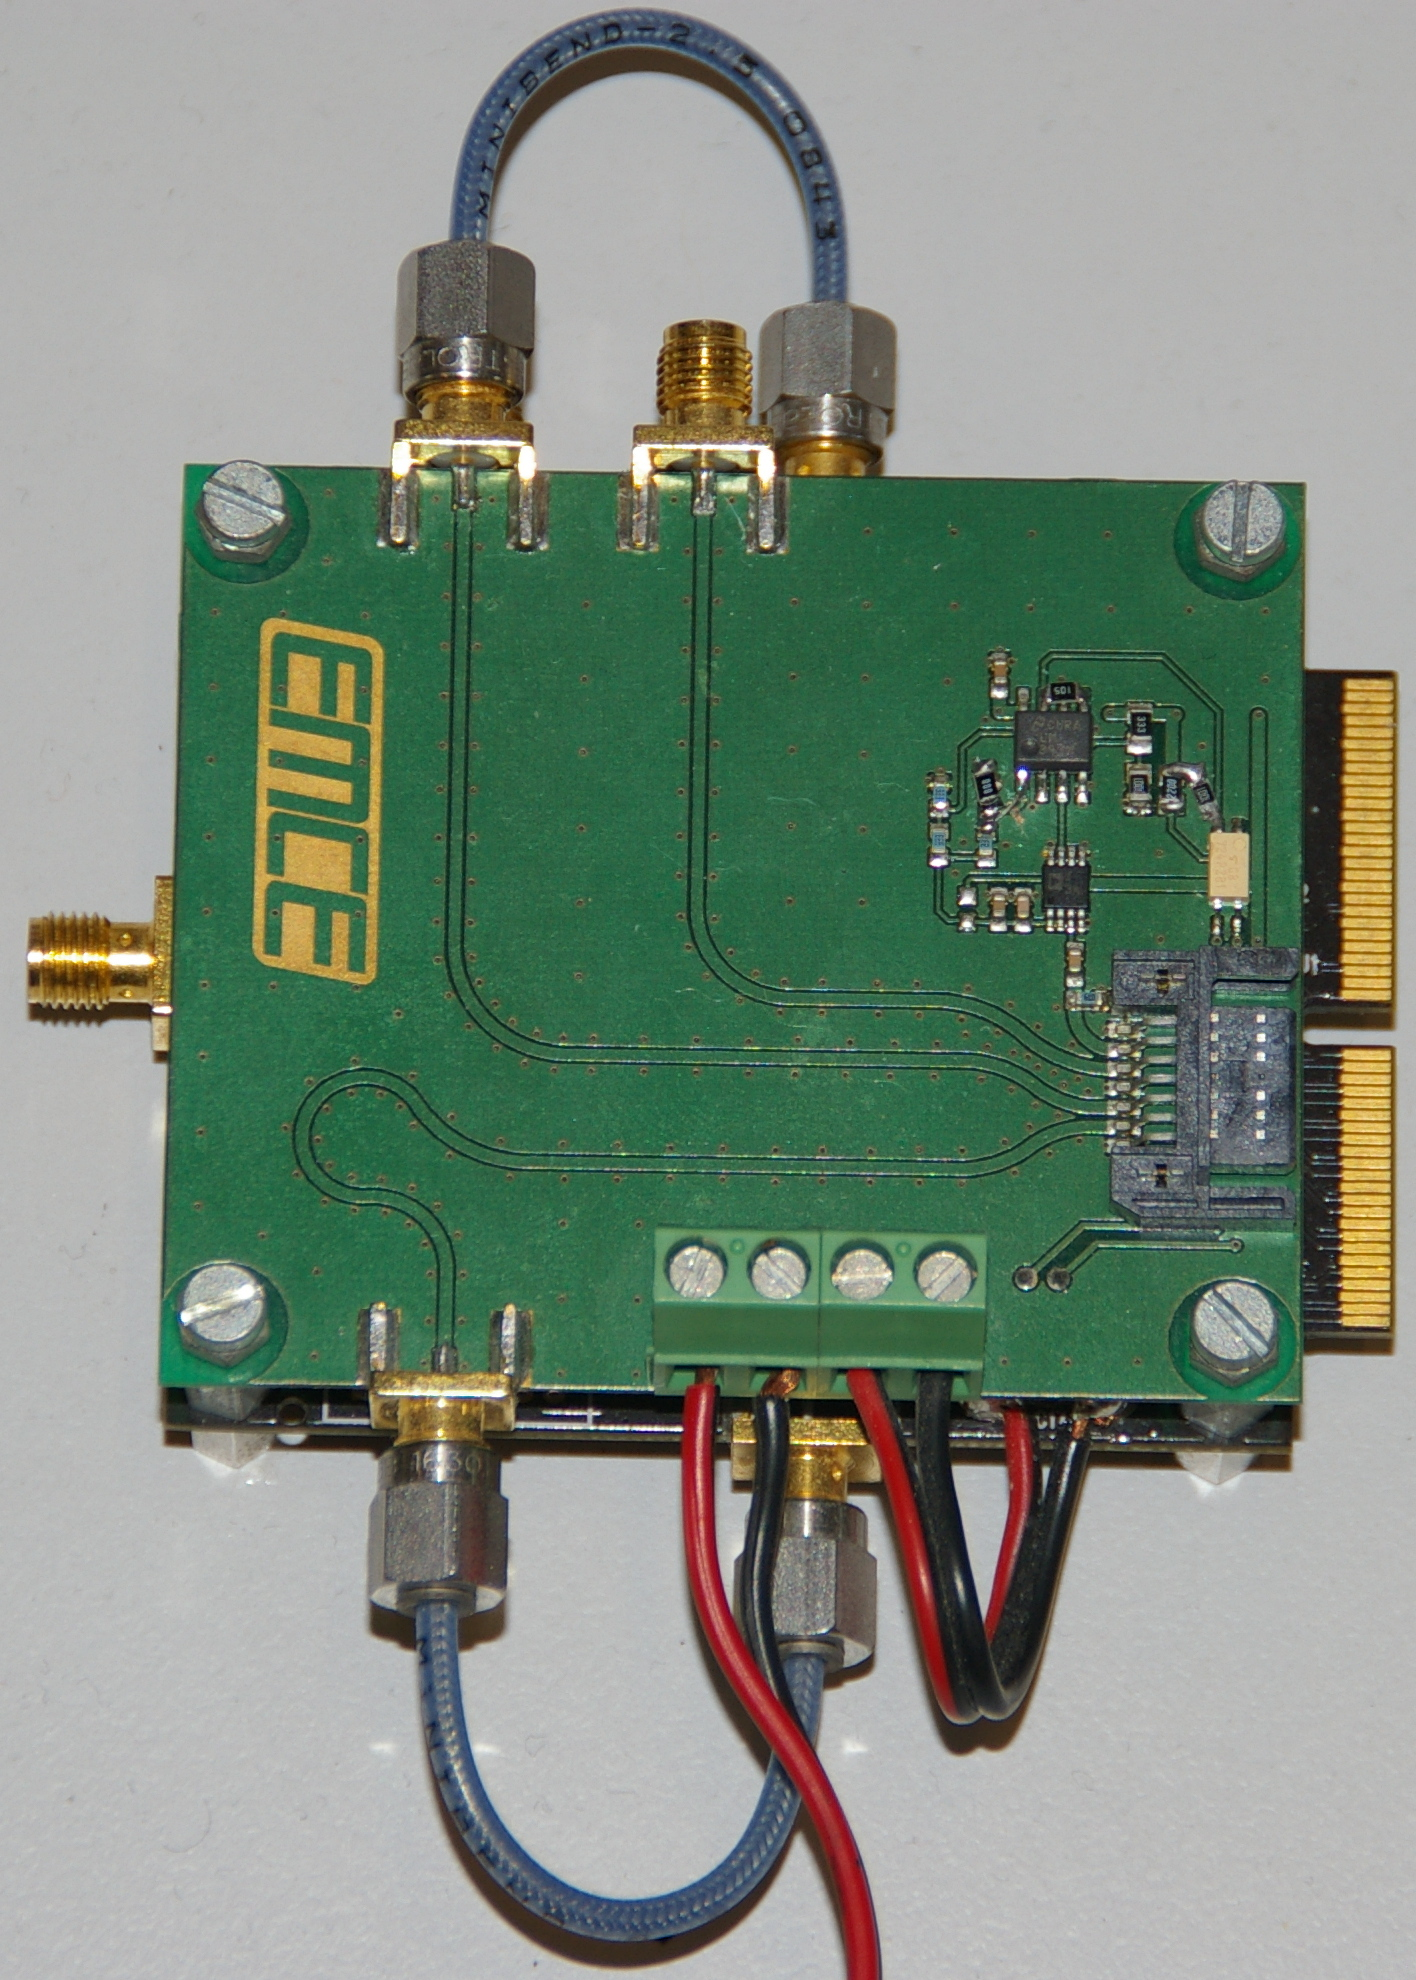
\includegraphics[width=\textwidth]{adc.jpg}};
            \begin{scope}[x={(image.south east)},y={(image.north west)},every node/.style={fill=white, fill opacity=0.8}]
                \draw (0,0.55) node[anchor=south west] {analog in};
                \draw (1,0) node[anchor=south east] {power supply};
                \draw (0.1,0.1) node[anchor=south west] {data+};
                \draw (0.1,0.9) node[anchor=north west] {data-};
                \draw (0.9,1) node[anchor=north east] (clk) {clock};
                \draw [-latex] (clk) -- (0.5,0.85);
                \draw (0.925,0.75) node[anchor=north east] {sync circuit};
                \draw (0.9,0.323) node[anchor=south east] {SATA};
            \end{scope}
        \end{tikzpicture}
        \caption{\glsentryshort{adc} adapter board with diconnected clock atop LTC2274 demo board}
        \label{fig:adc_adapter_circ}
    \end{subfigure}%
    ~
    \begin{subfigure}[c]{.49\linewidth}
        \centering
        \begin{tikzpicture}
            \node[inner sep=0pt] (image) at (0,0) {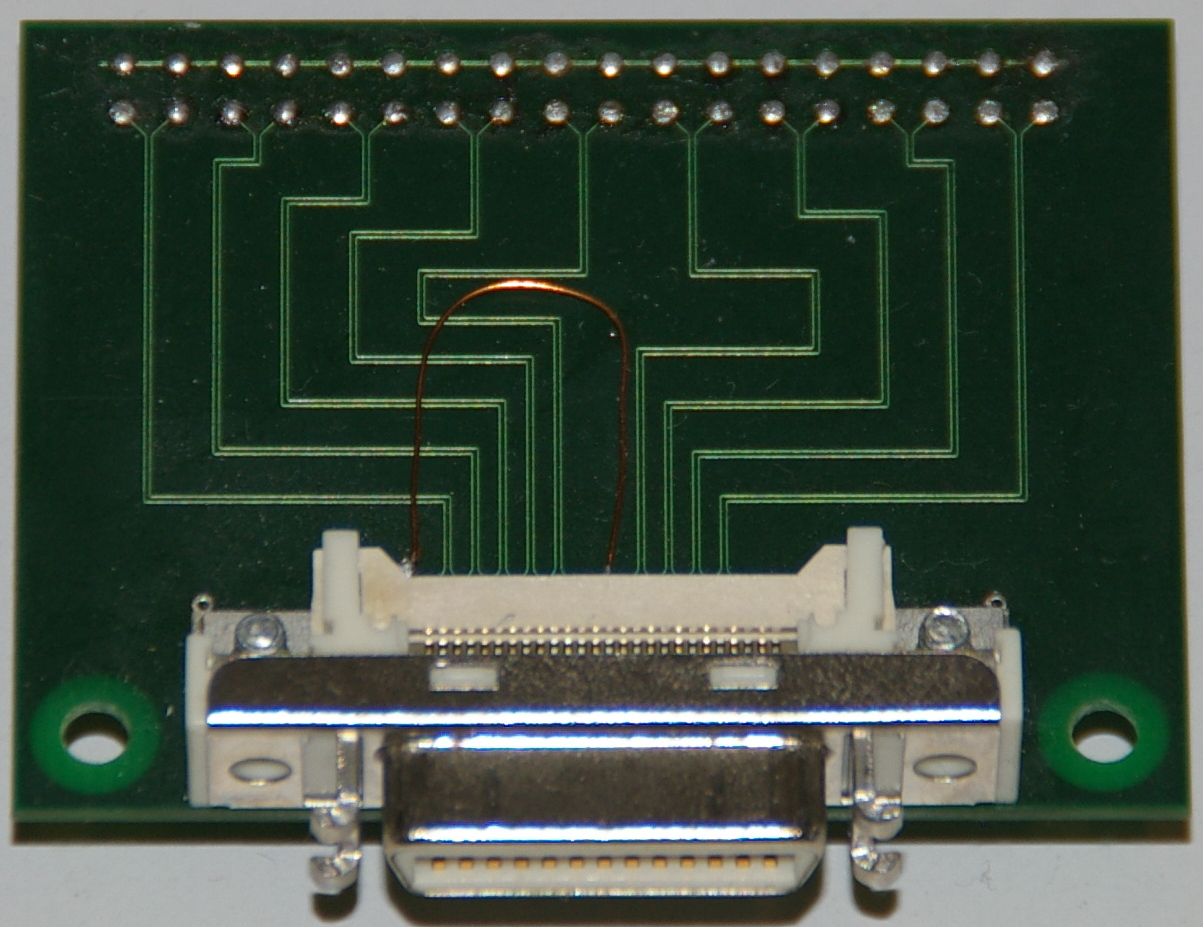
\includegraphics[width=\textwidth]{digital_iq.jpg}};
        \end{tikzpicture}
        \caption{Digital \glsentryshort{iq} adapter circuit board with S\_CLK fix}
        \label{fig:iq_adapter_circ}
    \end{subfigure}
    \caption{Photos of implemented adapter boards}
    \label{fig:adapters}
\end{figure}

The complete digital signal processing chain described in this section was implemented
in an \gls{fpga}. A detailed description of the digital hardware implementation can
be seen in \cref{chap:fpga}.

% ===========================================================================

\chapter{\glsentryshort{fpga} Implementation}
\label{chap:fpga}

The digital part, as described in \cref{sec:digital}, was realized in \gls{vhdl}.
It was specifically tailored to a Xilinx \mbox{Virtex-5} FXT on a ML507 evaluation board.
The \gls{fpga} model XC5VFX70T on this evaluation board provides the necessary
high speed transceivers, sufficient block \glspl{ram}, and dedicated digital
signal processing hardware \cite{virtex5ds}. Furthermore the ML507 board contains
an \gls{sata} connector needed for the \gls{adc} and pin headers with high speed differential signal routing to the \gls{fpga}
which can be used for the digital \gls{iq} interface. Additionally, the board contains an
Ethernet port enabling high speed data exchange with a \gls{pc}. Although, according to
\cite{ml507}, the \gls{sata} headers are only rated up to \SI{1.5}{\giga\bit\per\second},
it was confirmed during tests that the necessary \SI{2}{\giga\bit\per\second}, as required
by the \gls{adc} \cite{ltc2274}, are also technically feasible. This \gls{fpga} also contains a
hardwired PowerPC \gls{cpu}, which was used for controlling the digital components
and as a communication bridge to the \gls{pc}.

\tikzset{inbuf/.style={color=Set1-4-1}}
\tikzset{core/.style={color=Set1-4-2}}
\tikzset{outbuf/.style={color=Set1-4-3}}
\tikzset{pc/.style={color=Set1-4-4}}

\begin{figure}[htb]
    \centering
    \begin{subfigure}[c]{.69\linewidth}
        \centering
        \resizebox{\linewidth}{!}{
        \begin{tikzpicture}[every node/.style={minimum width=5em},latex-latex]
            \matrix (peripherals)[matrix of nodes,column sep=1.5em,row sep=0.2em,nodes={draw,anchor=center},ampersand replacement=\&]
            {
                DRAM \& \shortstack{DRAM\\Controller} \\
                |[pc]| Ethernet \& \shortstack{Ethernet\\Controller} \\
                |[pc]| RS232 \& \shortstack{RS232\\Interface} \\
                Storage \& Sys ACE \\
                \shortstack{LEDs\\Switches} \& GPIO \\
            };
            \node[draw,minimum size=5em,above right=0em of peripherals] (cpu) {CPU};
            \draw (peripherals-1-1) -- (peripherals-1-2);
            \draw (peripherals-1-2) -| ([xshift=-2.5em]cpu);
            \draw ([yshift=1em]peripherals-2-2) -| ([xshift=-1.5em]cpu);
            \foreach \i in {2,...,5}
            {
                \draw (peripherals-\i-1) -- (peripherals-\i-2);
                \draw (peripherals-\i-2) -- (peripherals-\i-2 -| cpu);
            }
            \draw[ultra thick,-] (peripherals-5-2 -| cpu) ++(0,-1em) node[below] (plb) {PLB} -- (cpu);
            \node[draw] at ($(peripherals-5-2)!2!(peripherals-5-2 -| cpu)$) (bram) {RAM};
            \draw (peripherals-5-2 -| cpu) -- (bram);
            \node[draw] at ($(peripherals-2-2)!2!(peripherals-2-2 -| cpu)$) (pint) {\shortstack{Processor\\Interface}};
            \draw (peripherals-2-2 -| cpu) -- (pint);
            \matrix (internal)[matrix of nodes,column sep=1em,row sep=0.2em,nodes={draw,anchor=center},right=of pint]
            {
                |[inbuf]| inbuf \\
                |[core]| core \\
                |[outbuf]| outbuf \\
                auto \\
            };
            \node[draw,right=1.5em of internal-3-1] (digiq) {Digital IQ};
            \node[draw,right=1.5em of internal-1-1] (adc) {ADC};
            \node[coordinate] at ($(pint.east) + (2em,0)$) (l) {};
            \foreach \i in {1,...,4}
            {
                \draw (pint.east) -- (l) |- (internal-\i-1);
            };
            \draw[inbuf,latex-] (internal-1-1) -- (adc);
            \draw[outbuf,-latex] (internal-3-1) -- (digiq);
            \node[draw,fit=(cpu) (peripherals-5-2) (plb) (bram),inner xsep=0.5em,label=processor] (processor) {};
            \node[coordinate] at ($(processor.north) + (0,1em)$) (u) {};
            \node[draw,fit=(internal-1-1) (internal-4-1) (l),inner xsep=0.5em,label=main] (main) {};
            \node[draw,fit=(processor) (main) (u),inner xsep=0.5em,label=top] (fpga) {};

        \end{tikzpicture}
        }
        \caption{\glsentryshort{fpga} modules and interconnections}
        \label{fig:fpga_modules}
    \end{subfigure}%
    ~
    \begin{subfigure}[c]{.29\linewidth}
        \centering
        \resizebox{\linewidth}{!}{
        \begin{tikzpicture}
            \tikzpicturedependsonfile{rfsymbols.tex}
            \tikzstyle{every node}=[font=\footnotesize]
            \draw (0,-1.5cm) node[coordinate,label=left:Dig IQ] (dac) {}

                  (0,1.5cm) node[coordinate,label=left:ADC] (adc) {}
                  node[empty,right=of adc,label=below:buffer1,inbuf] (inbuf) {}
                  node[mixer,right=of inbuf,core] (shift) {}
                  node[rotate=90,anchor=north] at (shift.east) {mix2}

                  (dac -| inbuf) node[mixer,label=above:mul1,outbuf] (mul) {}
                  node[empty,right=of mul,outbuf] (outbuf) {}
                  node[rotate=90,anchor=north] at (outbuf.east) {buffer2}

                  ($(shift)!.5!(outbuf)$) node[allpass,rotate=90,core] (H) {}
                  node[rotate=90,anchor=north] at (H.south) {fir1}

                  node[source,above=of shift.center,scale=0.7,core] (shiftsource) {}
                  node[rotate=90,anchor=south,font=\tiny] at (shiftsource.west) {$\SI{30}{\mega\hertz}$}
                  node[rotate=90,anchor=north] at (shiftsource.east) {lo3}
                  node[below=of mul.center,fill=white] (gamma) {$\glsdisp{GammaL}{\Gamma_{L,set}} = X + \gls{j}Y$};

            { [on background layer,every path/.style={dashed}]
                \draw ($(adc.east)!.5!(mul.west) + (0,4)$) -- ++(0,-8.5) node[coordinate] (rightsplit) {};
            }
            { [-latex]
                \draw [double,core] (shiftsource) -- (shift);
                \draw [outbuf,double] (gamma) -- (mul);
            }
            { [start chain,every on chain/.style={join=by -latex}]
                \chainin (adc);
                { [every on chain/.style={join=by {inbuf,-latex}}]
                    \chainin (inbuf);
                }
                \chainin (shift);
                { [every on chain/.style={join=by {double,-latex}}]
                    { [every on chain/.style={join=by {double,core,-latex}}]
                        \chainin (H);
                    }
                    \chainin (outbuf);
                    { [every on chain/.style={join=by {double,outbuf,-latex}}]
                        \chainin (mul);
                        \chainin (dac);
                    }
                }
            }

            \draw (rightsplit) node[anchor=base west] {Digital}
                  node[anchor=base east] {Analog};

            {[densely dashdotdotted,latex-latex,pc]
                \draw ($(inbuf.north) + (0,1)$) -- ++(0,1) node [anchor=south] {\acrshort{pc}};
            }
        \end{tikzpicture}
        }
        \caption{Digital signal processing chain}
        \label{fig:digital_chain}
    \end{subfigure}
    \caption[\glsentryshort{fpga} design overview and digital signal processing chain]{\glsentryshort{fpga} design overview and digital signal processing chain with color coded modules}
    \label{fig:fpga_overview}
\end{figure}

The design overview, as can be seen in \cref{fig:fpga_modules}, describes
the high level modules of the design and connections between them. Names used
in this and the following design overview are the actual module names used in the
source code. The overall
design was split into two parts. The digital signal processing chain
in \cref{fig:digital_chain} (see \cref{sec:digital}) implemented in the
\device{main} module. The \device{main} module is described in
\cref{sec:digital_processing}. The second part is the \device{processor} module
which contains a complete embedded processor system. This module was used to
implement the necessary protocols for communicating with a \gls{pc} in software.
It is described in \cref{sec:processor}.

This design uses the unrelated clocks from the \gls{plb} and the \gls{adc}.
Therefore clock synchronization was needed to minimize the chance of metastable
processes. This was achieved using a two-stage synchronizer as the base
synchronization circuit. Signals with short pulses were synchronized with an
additional pulse shaping to prevent lost pulses. Signal buses were synchronized
with an open loop approach. This approach leaves out the acknowledgement of the
synchronization which is sufficient for this design because the
\device{processor} module is not fast enough to change the bus value within the
synchronization period. Block \glspl{ram} in the used \gls{fpga} are true dual port
memories. Therefore no synchronization is necessary for read access. If one port
is used for writes to the memory the other port must not be used to access the same location at the same
time\cite{virtex5}. Care was taken to avoid this situation by disallowing
memory access from the other port during writes.

To ease software development a full \gls{os} was used as software for the
\gls{cpu}. Linux was chosen as the \gls{os} for the \device{processor} module, since
it is freely available and can be configured specifically for this target. As will
be discussed in \cref{sec:processor} the \device{processor} design includes the modules
needed to be able to use Linux. An overview of the complete Linux implementation
can be seen in \cref{chap:software}.

All hardware source codes and project files, which are needed to generate the hardware, can
be found in \cref{sec:sources}.

% ---------------------------------------------------------------------------

\section[Digital Signal Processing Chain]{Digital Signal Processing Chain --- main}
\label{sec:digital_processing}

The \device{main} module contains the digital signal processing chain. As can be seen
in \cref{fig:main_overview} the different parts of the processing chain (\cref{fig:digital_chain1}) are mapped
to three modules (\cref{fig:main}). The module \device{inbuf} contains the digital receive interface
for the \gls{adc} and the sample buffer \device{buffer1}. This module is described
in \cref{sec:acquisition}. The \device{core} module contains the frequency
mixer \device{mix2}, the \gls{lo} \device{lo3}, and the digital filter \device{fir1} with
the accompanying buffer \device{H} containing the transfer function $H\XN$.
A detailed description can be seen in \cref{sec:overlap_add}. The third part
is the \device{outbuf} module. This module contains the sample buffer \device{buffer2},
the multiplier \device{mul1}, and the digital \gls{iq} interface and is described in \cref{sec:smbv_interface}. The
filter \device{fir1} is not capable of handling a continuous data stream (see
\cref{sec:overlap_add}). Therefore the \device{auto} module was implemented to emulate
continuous behaviour by sequentially activating the modules \device{inbuf}, \device{core},
and \device{outbuf}. A more detailed description of the \device{auto} module can be seen
in \cref{sec:auto}.

\begin{figure}[htb]
    \centering
    \begin{subfigure}[c]{.49\linewidth}
        \centering
        \begin{tikzpicture}[every node/.style={minimum width=5em},latex-latex]
            \node[coordinate] (pint) {};
            \matrix (internal)[matrix of nodes,column sep=1em,row sep=0.2em,nodes={draw,anchor=center},right=of pint]
            {
                |[inbuf]| inbuf \\
                |[core]| core \\
                |[outbuf]| outbuf \\
                auto \\
            };
            \node[draw,right=1.5em of internal-3-1] (digiq) {Digital IQ};
            \node[draw,right=1.5em of internal-1-1] (adc) {ADC};
            \node[coordinate] at ($(pint.east) + (2em,0)$) (l) {};
            \foreach \i in {1,...,4}
            {
                \draw (pint) -- (l) |- (internal-\i-1);
            };
            \draw[inbuf,latex-] (internal-1-1) -- (adc);
            \draw[outbuf,-latex] (internal-3-1) -- (digiq);
            \node[draw,fit=(internal-1-1) (internal-4-1) (l),inner xsep=0.5em,label=main] (main) {};
            \node[fit=(main),inner xsep=0.5em] (fpga) {};
            \draw[dashed,-] ($(fpga.south east) - (0,1em)$) -- ($(fpga.north east)+(0,1em)$);

        \end{tikzpicture}
        \caption{Overview of the \device{main} module}
        \label{fig:main}
    \end{subfigure}%
    ~
    \begin{subfigure}[c]{.49\linewidth}
        \centering
        \begin{tikzpicture}
            \tikzpicturedependsonfile{rfsymbols.tex}
            \tikzstyle{every node}=[font=\footnotesize]
            \draw (0,-1.5cm) node[coordinate,label=left:Dig IQ] (dac) {}

                  (0,1.5cm) node[coordinate,label=left:ADC] (adc) {}
                  node[empty,right=of adc,label=below:buffer1,inbuf] (inbuf) {}
                  node[mixer,right=of inbuf,core] (shift) {}
                  node[rotate=90,anchor=north] at (shift.east) {mix2}

                  (dac -| inbuf) node[mixer,label=above:mul1,outbuf] (mul) {}
                  node[empty,right=of mul,outbuf] (outbuf) {}
                  node[rotate=90,anchor=north] at (outbuf.east) {buffer2}

                  ($(shift)!.5!(outbuf)$) node[allpass,rotate=90,core] (H) {}
                  node[rotate=90,anchor=north] at (H.south) {fir1}

                  node[source,above=of shift.center,scale=0.7,core] (shiftsource) {}
                  node[rotate=90,anchor=south,font=\tiny] at (shiftsource.west) {$\SI{30}{\mega\hertz}$}
                  node[rotate=90,anchor=north] at (shiftsource.east) {lo3}
                  node[below=of mul.center,fill=white] (gamma) {$\glsdisp{GammaL}{\Gamma_{L,set}} = X + \gls{j}Y$};

            { [on background layer,every path/.style={dashed}]
                \draw ($(adc.east)!.5!(mul.west) + (0,4)$) -- ++(0,-8.5) node[coordinate] (rightsplit) {};
            }
            { [-latex]
                \draw [double,core] (shiftsource) -- (shift);
                \draw [outbuf,double] (gamma) -- (mul);
            }
            { [start chain,every on chain/.style={join=by -latex}]
                \chainin (adc);
                { [every on chain/.style={join=by {inbuf,-latex}}]
                    \chainin (inbuf);
                }
                \chainin (shift);
                { [every on chain/.style={join=by {double,-latex}}]
                    { [every on chain/.style={join=by {double,core,-latex}}]
                        \chainin (H);
                    }
                    \chainin (outbuf);
                    { [every on chain/.style={join=by {double,outbuf,-latex}}]
                        \chainin (mul);
                        \chainin (dac);
                    }
                }
            }

            \draw (rightsplit) node[anchor=base west] {Digital}
                  node[anchor=base east] {Analog};

            {[densely dashdotdotted,latex-latex,pc]
                \draw ($(inbuf.north) + (0,1)$) -- ++(0,1) node [anchor=south] {\acrshort{pc}};
            }
        \end{tikzpicture}
        \caption{Digital signal processing chain}
        \label{fig:digital_chain1}
    \end{subfigure}
    \caption[\device{main} module overview and digital signal processing chain]{\device{main} module overview and digital signal processing chain with color coded modules}
    \label{fig:main_overview}
\end{figure}

Necessary bit width truncations throughout the digital signal processing chain use
convergent rounding. This rounding mode was used to prevent \gls{dc} offsets. It rounds
to even integers in case of a tie. For example rounding \num{4.5} with this method
results in \num{4}. The same would be true for \num{3.5}. Thus rounding does not introduce an offset towards infinity or zero, as would
be the case for round half up. Additionally, overflows are signalled and saturation is
used where applicable.

The sample buffer size was chosen according to the available block
\gls{ram} in the \gls{fpga}. A maximum number of \num{148} block \glspl{ram} capable of
storing up to \SI{36}{\kilo\bit} is available in the \mbox{Virtex-5} on the ML507 board\cite{virtex5ds}. Those block \glspl{ram}
can also be used as two independent \SI{18}{\kilo\bit} block \glspl{ram}. As
mentioned in \cref{sec:digital}, the digital signal processing chain needs to support a sample width
of \SI{16}{\bit}. Input averaging was chosen to support a maximum of \num{8} averages,
resulting in an overall needed bit with of \SI{19}{\bit} for the input buffer. Since
the output buffer uses double buffering and needs to store \gls{iq} signals,
two buffers with a bit width of \SI{32}{\bit} are needed. In order to achieve a high memory utilization,
constrained by the possible block \gls{ram} bit widths, a single data bit of a buffer was
realised with a \SI{36}{\kilo\bit} and a \SI{18}{\kilo\bit} block \gls{ram}. This leads
to a total number of \num{124.5} block \glspl{ram} where \num{0.5} denotes a
\SI{18}{\kilo\bit} block \gls{ram}. This leaves enough for the embedded processor
and the \gls{fft} implementation. Using this memory layout only a 2-to-1 multiplexer
for the output is needed. Since the highest address line can
be used as selection between both block \glspl{ram}, no address decoder is needed. This ensures fast operation of the
overall memory. In one bit mode only \SI{32}{\kilo\bit} (\SI{16}{\kilo\bit})
are available. This leads to a theoretical buffer depth of \num{49152} samples. However as
will be explained in \cref{sec:overlap_add} (see also \cref{sec:digital}), if circular convolution
with a block size of \gls{L} and an \gls{fft} size of $\gls{nfft}$ is used for the \gls{fir} filter,
the full buffer depth is not usable. This is caused by the implementation of the overlap add
algorithm which needs additional buffer space of $\gls{L} - \gls{nfft}$ samples after the signal.

The memory buses of the \device{inbuf} module and the \device{outbuf} module are
connected to the \device{core} module. The same bus connections are also exposed
via a memory interface of the \device{core} module. To prevent access violations
the exposed memory interface can't access the internal modules while one of
them is active. Also further module activations are not possible
during this period. With these restrictions in place no memory corruptions can
occur. The \device{core} module also exposes every configuration and status signal
of the internal modules. These signals are used by the processor interface described
in \cref{sec:processor_interface} for controlling the whole signal processing chain.

% ---------------------------------------------------------------------------

\subsection[Data Acquisition]{Data Acquisition --- inbuf}
\label{sec:acquisition}

The \device{inbuf} module is responsible for serial to parallel conversion
of the \gls{adc} data, descrambling, triggering, averaging, and storing
the acquired samples. As can be seen in \cref{fig:inbuf}, this module consists
of the main modules \device{receiver}, which handles receiving the data stream from
\gls{adc}, and \device{average\_mem}, which handles storing the samples in a buffer
and averaging. The additional modules \device{trigger}, \device{prepare}, and
\device{wallclk} are responsible for controlling the data acquisition and keeping
the time, which is needed for the \gls{iq} demodulation that will be explained in \cref{sec:overlap_add}.

\begin{figure}[htb]
    \centering
    \begin{tikzpicture}
        \foreach \i/\j in {0/2pt,1/0pt}
        {
            \begin{scope}[xshift=\j,yshift=\j,every node/.style={draw,fill=white}]
                \node (gtx\i) {GTX};
                \node[left=2em of gtx\i] (descramble\i) {descramble};
                \node[below=1em of gtx\i] (align\i) {align};
                \draw[latex-latex] (align\i) -- (gtx\i);
                \draw[-latex] (gtx\i) -- (descramble\i);
                \draw[latex-latex] (gtx\i.east) -- ++(2.5em,0); % node[draw,anchor=west] {adc};
            \end{scope}
        };
        \node[trapezium,rotate=90,anchor=center,draw,minimum height=1em] at ($(descramble0.west) + (-2em,-1pt)$) (mux) {};
        \draw[-latex] ([xshift=-2pt]descramble0.west) -- (mux.south |- descramble0);
        \draw[-latex] (descramble1.west) -- (mux.south |- descramble1);

        \node[fit=(descramble1) (gtx0) (align1),draw,label=receiver] (receiver) {};

        \node[circle,left=of mux.north,draw] (adder) {$+$};
        \draw[-latex] (mux) -- (adder);

        \node[draw,left=of adder] (memory) {memory};
        \draw[-latex] (adder) -- (memory);

        \draw[latex-latex] (memory.west) -- ++(-2em,0) node[coordinate] (out) {};
        \draw[-latex] (memory) -- ++(0,2em) node[coordinate] (upper) {} -| (adder);

        \node[fit=(memory) (adder) (upper),label=average\_mem,draw,inner xsep=0.5em] (average) {};
        \node[draw,anchor=west] at ($(average.south west) + (0,-2em)$) (prepare) {prepare};
        \node[draw,anchor=east] at ($(average.south east) + (0,-2em)$) (trigger) {trigger};

        \draw[-latex] (trigger) -- (average.south -| trigger);
        \draw[latex-latex] (prepare) -- (average.south -| prepare);

        \draw[-latex] (prepare) -- (trigger);
        \draw[latex-latex] (prepare) -- (prepare -| out);

        \node[draw,below=1em of trigger] (wallclk) {wallclk};
        \draw[-latex] (wallclk) -- (\currentcoordinate -| out);
        \draw[-latex] (trigger) -- (wallclk);

        \node[draw,fit=(average) (receiver) (trigger) (wallclk.north),inner ysep=2em,inner xsep=0.5em,label=inbuf] (inbuf) {};
        \draw[dashed] (inbuf.south east) ++(0.5em,-1em) -- (\currentcoordinate |- inbuf.north) -- ++(0,1em);

        \draw[dotted,-,decorate,decoration=random steps,segment length=2mm] ($(prepare)!.5!(trigger) - (0,6em)$) node[coordinate] (clk) {} |- ($(trigger.north) + (0,0.5em)$) -| ($(mux)!.5!(adder)$) -- ++(0,6em);
        \node[anchor=base east,font=\small] at (clk) {\gls{plb} clock};
        \node[anchor=base west,font=\small] at (clk) {\gls{adc} clock};
    \end{tikzpicture}
    \caption{Block diagram of the \device{inbuf} module}
    \label{fig:inbuf}
\end{figure}

The serial to parallel conversion was implemented using the built in GTX
transceiver. Since the ML507 board features two \gls{sata} ports, two
identical receivers were implemented. Since the GTX blocks need
a lot of configuration settings, they were instantiated using the
recommended method, which is the transceiver wizard documented in \cite{gtx_wizard}. The
settings used in this work were chosen according to the data sheet
of the \gls{adc} \cite{ltc2274}. The receiver was configured to handle the
specifications as described in the \cref{sec:digital}. These are 8b/10b line coding,
a data width of \SI{16}{\bit} and a target line rate of \SI{2}{\giga\bit\per\second}.
Synchronization was configured for an enabled idle synchronization mode (ISMODE) of the \gls{adc}. In this mode the
transmitter of the \gls{adc} sends idle ordered sets instead of commas during synchronization\cite{ltc2274}.
An idle ordered set is a special sequence used for synchronization consisting of a K28.5 comma
followed by either D5.6 or D16.2 code word. A comma is a special
code sequence of the 8b/10b line coding, which does not represent valid data\cite{gtx}.
To be able to synchronize the GTX receiver according to these specifications, the comma
alignment was set to align to even byte boundaries and to detect the K28.5 comma. After
serial to parallel conversion, the endianness is converted to the internal representation.
The recovered clock from the received data stream is used as the internal sampling clock.
This setup allows the use of an externally provided sampling clock, by connecting it to
the \gls{adc} instead of the clock provided by the \gls{adc} adapter circuit board
mentioned in \cref{sec:digital}. The receiver and
the transmitter share the internal clock generation of the GTX. Therefore the transmitter
had to be configured for the same line rate. To be able to transmit a clock signal with the
transmitter, the 8b/10b line coding was disabled for the transmitter and a fixed clock pattern was applied
to the parallel input.

It is not possible to provide an externally generated clock directly to the
\gls{sata} connected GTX transceivers, because of design limitations of the ML507 evaluation
board. Since using a clock, which is routed through the global clock
network of the \gls{fpga} introduces jitter \cite{gtx}, an externally provided sampling clock
connected to the \gls{adc} is the preferred mode of usage.

The module \device{align} controls the clock signal, which is transmitted using
the GTX. This module contains a state machine that blanks the clock signal
for \SI{41}{\milli\second} after a loss of sync of the receiver. In combination with the
synchronization circuit described in \cref{sec:digital} this clock blanking
enables synchronization mode for the \gls{adc}. A loss of sync is
detected if either a comma value or a value that is not part of the 8b/10b line coding
is detected. After the blanking period the clock signal is reactivated and
the GTX is put into alignment mode, which searches for the above mentioned comma
K28.5. If no comma is detected during a further \SI{41}{\milli\second} period the
synchronization re-starts from the beginning.

Succeeding the GTX transceiver, the \device{descrambler} module descrambles the data
according to the data sheet of the \gls{adc}\cite{ltc2274}. Data scrambling is
used to lessen the noise caused by the digital transmission in the analog part. The
scrambler implemented in the \gls{adc} is based on the generator polynomial given
in \cref{eq:poly} \cite{jesd205B.01}. This scrambler can be bypassed if a
different \gls{adc} is used.
\begin{equation}
    \label{eq:poly} g(x) = 1 + x^{14} + x^{15}
\end{equation}

Averaging the data is handled by the \device{average\_mem} module. This module
consists of the above mentioned \SI[product-units=brackets]{19 x 49152}{\bit} memory. Averaging is achieved
by reading the appropriate sample from the buffer and adding it to the current value.
For the first run the read sample is replaced with the value zero. Using this method
the sampled values are accumulated over a configurable number of zero, two,
four, or eight rounds. Averaging is achieved during memory access from outside the module
by shifting the accessed values by zero, one, two, or three bit. This is equal to dividing
the samples by the number of rounds used for averaging. This method needs to read
the sample from the last round from the buffer while writing the current sample
to the buffer. Therefore, both ports of the memory are needed by the implementation which
implies that the synchronization technique using different ports for the different clock
domains as described above is not feasible. Hence, the memory interface allowing
access to the sample buffer from outside the \device{inbuf} module needs to share
the ports with the averaging mechanism. Since those two parts don't share the same
clock, clock multiplexing with dedicated \gls{fpga} hardware was implemented.

If the data acquisition is not in use, the \device{average\_mem} is powered by
the \gls{plb} clock. Before data acquisition, the \device{prepare} module
transitions the clock signal to the \gls{adc} clock. Undefined behaviour can
occur if the timing conditions of the address signals of the block \gls{ram}
are violated while the enable signal is high. This can lead to memory corruption
even if write enable is not asserted\cite{virtex5}. Therefore, the enable signal
of the block \gls{ram} is switched to low by the \device{prepare} module before
the clock transition. Since this is not possible for an unstable \gls{adc} clock,
the validity of the sample buffers is not guaranteed after connecting or
disconnecting an \gls{adc}. After the data acquisition finishes, the
\device{prepare} module transitions the clock signal back to the \gls{plb} clock.
Write operations to the memory are ignored during data acquisition. Read operations
during data acquisition don't interfere with the process but the read out data is invalid.

The \device{trigger} module generates the start signal for the \device{average\_mem}
and the \device{wallclk} module. During the first run and after a reset, the trigger can either be triggered
externally or internally. The external trigger is sampled from the pin AN33 of the
\gls{fpga}, which is connected to HDR1\_64 on the evaluation board. After the first
successful trigger, consecutive triggers are only generated at multiples of the configured signal period \gls{N}.

Subsequent to a trigger event, the \device{wallclk} module takes a snapshot of the
jiffy counter which marks the time the first sample of the current acquisition
was acquired. A jiffy is \SI{10}{\nano\second} in this \gls{fpga} design which is the time needed for
one sample for a sample period of \SI{100}{\mega\hertz}. The \SI{30}{\mega\hertz} signal for the \gls{iq} demodulation
is not generated in real time. Therefore the snapshot of the jiffy counter is necessary
for the \device{core} module to generate the \SI{30}{\mega\hertz} signal with the
correct phase (see \cref{sec:digital,sec:overlap_add}).

The \device{inbuf} module is fully runtime configurable. Changing the active receiver
or connecting an \gls{adc} resets the whole module automatically. This prevents undefined
behaviour which could result from the clock change. Since the trigger source is only
decisive for the first trigger event changing the source is only possible if the \device{trigger}
module has not fired yet. Therefore, the trigger module should be reset after changing
the source. Trigger events, averaging finished, and \gls{adc} connection status are reported
with separate signals. The memory interface of the \device{inbuf} module has a \SI{16}{\bit} wide data bus,
a \SI{16}{\bit} wide address bus, and a read access latency of 2 cycles. Accessing samples
at addresses \num{>= 49152} result in undefined behaviour.

% ---------------------------------------------------------------------------

\subsection[Overlap Add]{Overlap Add --- core}
\label{sec:overlap_add}

An overview of the \device{core} module can be seen in \cref{fig:core}.
It consists of the buffer \device{H}, which is needed to store the transfer
function, and the module \device{overlap\_add}, which contains the signal
processing. The \device{overlap\_add}
module itself contains the module \device{wave}, which is responsible for \gls{iq}
demodulation, the \device{fft} module, which can calculate the \gls{fft} and
inverse-\gls{fft}, a complex adder, a complex multiplier, and additional block
\gls{ram}, needed as temporary buffer space (\device{scratch}).

\begin{figure}[htb]
    \centering
    \begin{tikzpicture}
        \node[source] (source) {};
        \node[circle,draw,below=1em of source] (wavemul) {$\times$};
        \draw[double,-latex] (source) -- (wavemul);
        \draw[latex-] (source.west) -- ++(-2em,0) node[coordinate] (out) {};
        \draw[latex-] (wavemul.west) -- (\currentcoordinate -| out);

        \node[draw,fit=(wavemul) (source),inner xsep=0.5em,label=below:wave] (wave) {};

        \node[draw,right=4em of wavemul] (fft) {fft};
        \draw[double,-latex] (wavemul) -- (fft);

        \node[circle,draw,right=4em of fft] (mul) {$\times$};
        \node[draw,above=5em of mul] (H) {H};
        \draw[double,latex-latex] (H) -- (\currentcoordinate -| out);

        \draw[double,-latex] (H) -- (mul);
        \draw[double,-latex] (fft) -- (mul);

        \node[draw,right=of mul] (scratch) {scratch};
        \draw[double,-latex] (mul) -- (scratch);
        \draw[double,-latex] (scratch.east) -| ++(1em,2em) -| ($(fft.west) - (1em,0)$) -- (fft);

        \node[circle,draw,below=1em of scratch] (add) {$+$};

        \draw[double,-latex] (scratch.east) -- ++(1em,0) node[coordinate] (r) {} |- (add);
        \draw[double,-latex] (fft.east) -- ++(2em,0) |- (add);
        \draw[double,-latex] (fft.east) -- ++(2em,0) -- (\currentcoordinate |- add) -| ($(mul.east)!.5!(scratch.west)$) -- (scratch);

        \draw[double,-latex] (add.south) -- ++(0,-1em) node[coordinate] (d) {} -- (\currentcoordinate -| out);
        \draw[double,latex-latex] (scratch) -- ($(mul.east)!.5!(scratch.west)$) -- (\currentcoordinate |- d) -- (\currentcoordinate -| out);

        \node[draw,fit=(wave) (add) (scratch) (r) (d),label={[xshift=8em]overlap\_add}] (overlap) {};
        \node[draw,fit=(overlap) (H),label=core] (core) {};
    \end{tikzpicture}
    \caption{Block diagram of the \device{core} module}
    \label{fig:core}
\end{figure}

The \gls{iq} demodulation module \device{wave} consists of a hard coded look up
table, that generates a \SI{30}{\mega\hertz} sine and cosine waveform for
a sampling rate of \SI{100}{\mega\hertz}. Furthermore it contains multipliers,
which multiply the incoming samples with the sine and cosine waveforms, for
converting the signal into I and Q samples. Instead of performing this demodulation
in real time, it is performed during filter processing. To ensure the correct phase
of the \SI{30}{\mega\hertz} waveform it is evaluated at the point in time calculated
from the jiffy counter and the position of the currently processed sample. The jiffy
counter is contained in the \device{wallclk} module as explained in
\cref{sec:acquisition}. This counter marks the time the first sample of the current
signal was taken.

A Xilinx LogiCore IP was used as the \device{fft} module \cite{xilinx_fft}. In
order to minimize block \gls{ram} usage and increase the performance the
pipelined version was used. A further reduction in block \gls{ram} usage was achieved
by limiting the IP core to the minimum setting of three stages in block \gls{ram}. The
remaining stages needed for this configuration are implemented in distributed \gls{ram} which
results in a higher \gls{lut} usage of the \device{fft}\cite{xilinx_fft,virtex5}. Distributed
\gls{ram} was preferred over block \gls{ram} because \gls{lut} usage was not a limiting factor
in this design. The \device{fft} implementation was set to allow a modification of the
\gls{fft} length at runtime, with a maximum length of \num{4096}. A further runtime configuration
setting is, that this core can be switched between \gls{fft} and inverse \gls{fft}. This
allowed using only one \device{fft} module, therefore reducing the resource usage further. Every
computational part of the \gls{fft}, called a butterfly, consists of an addition and a multiplication
that preserves the magnitude of the complex valued input of the butterfly. The addition
increases the needed bit width after every butterfly by one bit to be able to represent every
possible value. The multiplication can result in an overall bit with growth of one bit for the
whole \gls{fft} if the magnitude represented by the complex valued input is greater than one.
Combining both factors leads to \cref{eq:bit_growth} given in \cite{xilinx_fft}.
\begin{equation}
    \label{eq:bit_growth}
    bits_{out} = bits_{in} + \underbrace{\log_2\left(\gls{nfft}\right)}_{\text{addition per butterfly}} + \underbrace{1}_{\text{complex rotation}}
\end{equation}
According to \cref{eq:bit_growth}, keeping every bit for an \gls{fft} length $\gls{nfft}$ of \num{4096}
and input width $bits_{in}$ of \SI{16}{\bit} would result in a maximum output width $bits_{out}$
of \SI{29}{\bit}. Using such high bit widths is not possible because of resource constraints.
Therefore, scaling was used and is implemented with a divider after every group, where one group
consists of two butterflies. Every divider can divide the samples by one, two, four, or eight.
Since the possibility of overflows depends on the input data the right scaling schedule can't
be determined beforehand. According to \cite{xilinx_fft} the best scaling schedule for the
\gls{fft} and inverse \gls{fft} is found by starting with a divider schedule of one and incrementing
the divider schedule until the computation stops overflowing. Input data for the \gls{fft} core
needs to be in natural order and output data is in bit reversed order \cite{xilinx_fft}.

The complex multiplier was implemented with a runtime changeable scaling schedule. This
schedule can be set to shift the result by \num{14} to \num{17} bits. Therefore, the transfer function
should always be scaled to the maximum possible values. The best overall scaling schedule
can be found by first configuring the scaling schedule of the \gls{fft}, then the
complex multiplier and after that the inverse \gls{fft}.

\begin{figure}[htb]
    \centering
    \begin{subfigure}[t]{.49\linewidth}
        \centering
        \resizebox{\linewidth}{!}{
        \begin{tikzpicture}[gray]
            \node[draw,black] (wave) {wave};
            \draw[latex-,red] (wave.west) -- ++(-1em,0) node[coordinate] (out) {} node[left] {$x$};

            \node[draw,right=2em of wave,black] (fft) {fft};

            \node[circle,draw,right=2em of fft] (mul) {$\times$};
            \node[coordinate,above=1.5em of mul] (u) {};
            \node[above=3em of mul] (H) {$H$};

            \draw[double] (H) -- (mul);
            \draw[double] (fft) -- (mul);

            \node[draw,right=of mul] (scratch) {scratch};
            \draw[double] (mul) -- (scratch);
            \draw[double] (scratch.east) -| ++(1em,2em) -| ($(fft.west) - (1em,0)$) -- (\currentcoordinate |- fft);

            \node[circle,draw,below=1em of scratch] (add) {$+$};

            \draw[double] (scratch.east) -- ++(1em,0) node[coordinate] (r) {} |- (add);
            \draw[double] (fft.east) -- ($(fft.east)!.5!(mul.west)$) |- (add);
            \draw[double] (fft.east) -- ($(fft.east)!.5!(mul.west)$) -- (\currentcoordinate |- add) -| ($(mul.east)!.5!(scratch.west)$) -- (scratch);

            \draw[double] (add.south) -- ++(0,-1em) node[coordinate] (d) {} -- (\currentcoordinate -| out) node[left] {$y$};
            \draw[double] (scratch) -- ($(mul.east)!.5!(scratch.west)$) -- (\currentcoordinate |- d) -- (\currentcoordinate -| out);

            \node[draw,fit=(wave) (add) (scratch) (r) (d) (u),inner xsep=0.5em,black] (overlap) {};
            \node[black,anchor=south east] at (overlap.north east) {overlap\_add};
            \draw[double,-latex,red] (wave) -- (fft);
        \end{tikzpicture}
        }
        \caption{Step 1: Up converting and filling \device{fft} with samples.}
        \label{fig:stage1}
    \end{subfigure}%
    ~
    \begin{subfigure}[t]{.49\linewidth}
        \centering
        \resizebox{\linewidth}{!}{
        \begin{tikzpicture}[gray]
            \node[draw] (wave) {wave};
            \draw (wave.west) -- ++(-1em,0) node[coordinate] (out) {} node[left] {$x$};

            \node[draw,right=2em of wave,black] (fft) {fft};
            \draw[double] (wave) -- (fft);

            \node[circle,draw,right=2em of fft,black] (mul) {$\times$};
            \node[coordinate,above=1.5em of mul] (u) {};
            \node[above=3em of mul,red] (H) {$H$};

            \node[draw,right=of mul,black] (scratch) {scratch};
            \draw[double] (scratch.east) -| ++(1em,2em) -| ($(fft.west) - (1em,0)$) -- (fft);

            \node[circle,draw,below=1em of scratch] (add) {$+$};

            \draw[double] (scratch.east) -- ++(1em,0) node[coordinate] (r) {} |- (add);
            \draw[double] (fft.east) -- ($(fft.east)!.5!(mul.west)$) |- (add);
            \draw[double] (fft.east) -- ($(fft.east)!.5!(mul.west)$) -- (\currentcoordinate |- add) -| ($(mul.east)!.5!(scratch.west)$);

            \draw[double] (add.south) -- ++(0,-1em) node[coordinate] (d) {} -- (\currentcoordinate -| out) node[left] {$y$};
            \draw[double] ($(mul.east)!.5!(scratch.west)$) -- (\currentcoordinate |- d) -- (\currentcoordinate -| out);

            \node[draw,fit=(wave) (add) (scratch) (r) (d) (u),inner xsep=0.5em,black] (overlap) {};
            \node[black,anchor=south east] at (overlap.north east) {overlap\_add};
            \draw[double,-latex,red] (fft) -- (mul);
            \draw[double,-latex,red] (mul) -- (scratch);
            \draw[double,-latex,red] (H) -- (mul);
        \end{tikzpicture}
        }
        \caption{Step 2: Unloading \device{fft} and complex multiplication.}
        \label{fig:stage2}
    \end{subfigure}\\
    \begin{subfigure}[t]{.49\linewidth}
        \centering
        \resizebox{\linewidth}{!}{
        \begin{tikzpicture}[gray]
            \node[draw] (wave) {wave};
            \draw[latex-] (wave.west) -- ++(-1em,0) node[coordinate] (out) {} node[left] {$x$};

            \node[draw,right=2em of wave,black] (fft) {ifft};
            \draw[double] (wave) -- ($(fft.west) - (1em,0)$);

            \node[circle,draw,right=2em of fft] (mul) {$\times$};
            \node[coordinate,above=1.5em of mul] (u) {};
            \node[above=3em of mul] (H) {$H$};

            \draw[double] (H) -- (mul);
            \draw[double] (fft) -- (mul);

            \node[draw,right=of mul,black] (scratch) {scratch};
            \draw[double] (mul) -- ($(mul.east)!.5!(scratch.west)$);

            \node[circle,draw,below=1em of scratch] (add) {$+$};

            \draw[double] (scratch.east) -- ++(1em,0) node[coordinate] (r) {} |- (add);
            \draw[double] (fft.east) -- ($(fft.east)!.5!(mul.west)$) |- (add);
            \draw[double] (fft.east) -- ($(fft.east)!.5!(mul.west)$) -- (\currentcoordinate |- add) -| ($(mul.east)!.5!(scratch.west)$);

            \draw[double] (add.south) -- ++(0,-1em) node[coordinate] (d) {} -- (\currentcoordinate -| out) node[left,blue] {$y$};
            \draw[double,latex-,blue] (scratch) -- ($(mul.east)!.5!(scratch.west)$) -- (\currentcoordinate |- d) -- (\currentcoordinate -| out);

            \node[draw,fit=(wave) (add) (scratch) (r) (d) (u),inner xsep=0.5em,black] (overlap) {};
            \node[black,anchor=south east] at (overlap.north east) {overlap\_add};
            \draw[double,-latex,red] (scratch.east) -| ++(1em,2em) -| ($(fft.west) - (1em,0)$) -- (fft);
        \end{tikzpicture}
        }
        \caption{Step 3: Loading the \device{fft} with the computed samples and loading scratch with the previous block.}
        \label{fig:stage3}
    \end{subfigure}%
    ~
    \begin{subfigure}[t]{.49\linewidth}
        \centering
        \resizebox{\linewidth}{!}{
        \begin{tikzpicture}[gray]
            \node[draw] (wave) {wave};
            \draw[latex-] (wave.west) -- ++(-1em,0) node[coordinate] (out) {} node[left] {$x$};

            \node[draw,right=2em of wave,black] (fft) {ifft};
            \draw[double] (wave) -- (fft);

            \node[circle,draw,right=2em of fft] (mul) {$\times$};
            \node[coordinate,above=1.5em of mul] (u) {};
            \node[above=3em of mul] (H) {$H$};

            \draw[double] (H) -- (mul);
            \draw[double] (fft) -- (mul);

            \node[draw,right=of mul,black] (scratch) {scratch};
            \draw[double] (mul) -- (scratch);
            \draw[double] (scratch.east) -| ++(1em,2em) -| ($(fft.west) - (1em,0)$) -- (fft);

            \node[circle,draw,below=1em of scratch,black] (add) {$+$};

            \draw[double] (fft.east) -- ($(fft.east)!.5!(mul.west)$) -- (\currentcoordinate |- add) -| ($(mul.east)!.5!(scratch.west)$) -- (scratch);

            \draw[double,-latex,red] (scratch.east) -- ++(1em,0) node[coordinate] (r) {} |- (add);
            \draw[double,-latex,red] (add.south) -- ++(0,-1em) node[coordinate] (d) {} -- (\currentcoordinate -| out) node[left] {$y$};
            \node[draw,fit=(wave) (add) (scratch) (r) (d) (u),inner xsep=0.5em,black] (overlap) {};
            \draw[double] (scratch) -- ($(mul.east)!.5!(scratch.west)$) -- (\currentcoordinate |- d);
            \node[black,anchor=south east] at (overlap.north east) {overlap\_add};
            \draw[double,-latex,red] (fft.east) -- ($(fft.east)!.5!(mul.west)$) |- (add);
        \end{tikzpicture}
        }
        \caption{Step 4: Unloading \device{fft} and adding the overlapping part from \device{scratch}.}
        \label{fig:stage4}
    \end{subfigure}
    \caption{Overlap add algorithm hardware implementation}
    \label{fig:overlap_add_machine}
\end{figure}

The overlap add algorithm, as explained in \cref{sec:digital}, was implemented with
two separate state machines. This allows speeding up the process since some parts can be calculated in parallel.
The first state machine controls the \gls{fft} and the complex multiplication part of the
algorithm. It is called \device{fftncmul}. Inverse \gls{fft} and complex
addition is handled by \device{ifftnadd}. The overall process is described in
\cref{fig:overlap_add_machine}. Every block of size \gls{L}
needs to be processed within four steps. In the first step (\cref{fig:stage1}),
the \device{fft} module is loaded with \gls{L} \gls{iq} demodulated samples from the source memory $x$. According to
the overlap add algorithm, after \gls{L} samples the data input of the \device{fft}
is switched to zero. After the \device{fft} module has finished processing,
the second step (\cref{fig:stage2}) starts. In this step the data is multiplied
with $H$ and stored in the scratch buffer. During the next step (\cref{fig:stage3}),
the \device{fft} module is switched to inverse operation and the samples from the
\device{scratch} buffer are loaded into the \device{fft} module. At the same time
the \device{scratch} buffer is filled with the previous computed block from the target
memory $y$. After the \device{fft} module has finished the computation, the last step (\cref{fig:stage4})
is executed. During this step the overlapping part from the previous block is added and
the samples are unloaded into the target memory. Since the \gls{fft}
module is pipelined, step one of the next block is started after step three
of the current block has finished. This means, that the \gls{fft} module computes
the samples of two different blocks at the same time. With this technique, the
duration of the overlap add algorithm is reduced by one stage per \gls{L} sized block.
If the circular mode is enabled, then the block after the signal is added to the
beginning (see \cref{sec:digital}). Since this process needs $\gls{L} - \gls{nfft}$ samples
after the end of the signal, the sample buffer can't be used to the full extent.

The overall module is freely configurable and accepts \gls{fft} sizes \num{8}, \num{16},
\num{32}, \num{64}, \num{128}, \num{256}, \num{512}, \num{1024}, \num{2048}, and \num{4096}.
The signal size \gls{N} has to be between \num{8} and \num{65535} and the block size
\gls{L} between \num{1} and \num{4096}. There are no plausibility
checks in the hardware, which means that wrong settings will lead to undefined
behaviour. The \device{core} module can be stopped by issuing a reset signal.
Numerical overflows are separately reported for \gls{fft}, inverse \gls{fft}
and complex multiplication.

% ---------------------------------------------------------------------------

\subsection[Vector Signal Generator Interface]{Vector Signal Generator Interface --- outbuf}
\label{sec:smbv_interface}

The \device{outbuf} module consists of two independent sample buffers
\device{mem\_0} and \device{mem\_1}, a complex multiplier and the digital
\gls{iq} interface \device{transmitter}. The two sample buffers are both
\SI{32}{\bit} wide, to store the \SI{16}{\bit} wide I and Q
signals. Both can store up to \num{49152} samples. A general overview can be
seen in \cref{fig:outbuf}.

\begin{figure}[htb]
    \centering
    \begin{tikzpicture}
        \node[draw,fill=white] (mem0) {mem\_0};
        \node[draw,below=of mem0,fill=white] (mem1) {mem\_1};
        \node[coordinate] at ($(mem0.west)+(-4em,0)$) (out) {};

        \draw[double] ($(mem0.west)-(1em,0)$) -- ($(mem1.west)-(2em,0)$)  node[coordinate] (out2) {};
        \draw[double] ($(mem1.west)-(1em,0)$) -- ($(mem0.west)-(2em,0)$);
        \draw[double,latex-latex] (mem0.west) -- (out);
        \draw[double,latex-latex] (mem1) -- (mem1 -| out);

        \node[trapezium,minimum height=1em,rotate=-90,anchor=center,draw] at ($(mem0.south east)!0.5!(mem1.north east) + (3em,0)$) (mux) {};

        \draw[double,-latex] (mem0.east) -| ([yshift=0.5em]$(mux.south) - (1em,0)$) -- ([yshift=0.5em]mux.south);
        \draw[double,-latex] (mem1.east) -| ([yshift=-0.5em]$(mux.south) - (1em,0)$) -- ([yshift=-0.5em]mux.south);

        \node[circle,draw,right=of mux.north] (mul) {$\times$};
        \draw[double,-latex] (mux) -- (mul);
        \draw[double,latex-] (mul.south) -- ++(0,-3em) node[coordinate] (r) {} -- (\currentcoordinate -| out);

        \node[draw,right=of mul] (transmitter) {transmitter};
        \draw[double,-latex] (mul) -- (transmitter);
        \draw[double,-latex] (transmitter.east) -- ++(2em,0);

        \node[draw,fit=(mem0) (r) (transmitter) (out2),inner xsep=0.5em,label=outbuf] (outbuf) {};
        \draw[dashed] (outbuf.south east) ++(0.5em,-1em) -- (\currentcoordinate |- outbuf.north) -- ++(0,1em);

        {[on background layer]
            \draw[dotted,-,decorate,decoration=random steps,segment length=2mm] ($(mem0.center) - (0,8em)$) node[coordinate] (clk) {} -- ($(mem0.center) + (0,3em)$);
            \node[anchor=base east,font=\small] at (clk) {\gls{plb} clock};
            \node[anchor=base west,font=\small] at (clk) {\gls{adc} clock};
        }
    \end{tikzpicture}
    \caption{Block diagram of the \device{outbuf} module}
    \label{fig:outbuf}
\end{figure}

Sample buffers \device{mem\_0} and \device{mem\_1} can only be accessed by the
logical names \device{active} and \device{inactive} from outside the
\device{outbuf} module. The \device{active} sample buffer contains the sample data,
which is streamed via the \device{transmitter} module to the digital \gls{iq}
interface. This memory can only be used in read mode via the internal interface.
The \device{inactive} sample buffer can be read and written to. Maintaining this
logical to physical assignment is handled by the network, indicated to the left
of the sample buffers, and the multiplexer in \cref{fig:outbuf}. Both sample
buffers consist of true dual port block \glspl{ram}. In combination with the
unsupported writes to the \device{active} sample buffer, this ensures that
no timing conditions are violated, due to the different clocks.

The \device{outbuf} module uses a configurable signal period \gls{N}. This period can only be changed
by resetting the module or by asserting the \device{resync} signal. Sample data of length \gls{N} is
continuously read from the \device{active} buffer. Swapping the \device{active}
and the \device{inactive} buffer can be initiated by asserting the toggle\_buf
signal for one cycle. To prevent signal distortion, the actual swapping occurs
only before reading sample zero from the buffer. Accesses to the sample buffers
during this operation result in undefined behaviour and can corrupt the buffer
content. This is prevented by the access protection mechanism implemented
in the \device{core} module.

The complex multiplier, between the multiplexer and the \device{transmitter}
module in \cref{fig:outbuf}, is responsible for the
reflection generation. It multiplies the signal output to the transmitter
with $\glsdisp{GammaL}{\Gamma_{L,set}}$ (see \cref{sec:digital}). As mentioned earlier, this
multiplier features a bit shifter at the output. This bit shifter shifts the
output by a configurable range of \SIrange{2}{17}{\bit}. With that operation
it is possible to reach full scale output also for small input
signals. This is necessary if, for example, a high scaling factor is needed
for the \device{core} module (see \cref{sec:overlap_add}). After this scaling
and convergent rounding, the multiplier is also capable of saturating the
output. This would prevent a wrap around and therefore limit signal distortion.

According to \cite{fsq_b17} the Rohde \& Schwarz digital \gls{iq} interface
uses the encoding scheme and digital interface of a DS90CR485 channel link
serializer. This serializer encodes data from a \SI{24}{\bit} input on both
clock edges resulting in a total of \SI{48}{\bit} per clock cycle \cite{ds90cr485}.
As specified by \cite{fsq_b17} \SI{20}{\bit} I data, \SI{20}{\bit} Q data, enable,
valid, marker bits, and trigger bits need to be encoded in these \SI{48}{\bit}. Enable
and valid are connected to high in this implementation. The marker and trigger
bits are not supported by the Rohde \& Schwarz SMBV100A vector signal generator
in digital \gls{iq} input mode. Therefore these were permanently disabled in this
work. The \gls{fpga} internal \SI{16}{\bit} \gls{iq} implementation was mapped
onto the \SI{20}{\bit} link by left shifting the data by \SI{4}{\bit}.

The \device{transmitter} module is an implementation of the DS90CR485 channel
link serializer specification in \gls{vhdl}. Since \cite{fsq_b17} does not
mention which operating mode of the channel link serializer is needed, the
full DS90CR485 specification according to \cite{ds90cr485} was implemented during this work.
According to this specification, the \SI{48}{\bit}, as mentioned in the last
paragraph, need to be partitioned onto eight \gls{lvds} links clocked at
\SI{700}{\mega\hertz}. It is not possible to achieve such high frequencies
in the \gls{fpga} fabric. Therefore the serialization was implemented utilizing
\glspl{oserdes} in \SI{4}{\bit} \gls{ddr} mode. The \gls{ddr} mode reduces the
necessary clock rate to \SI{350}{\mega\hertz} for the \gls{oserdes}. Furthermore the
\SI{4}{\bit} mode decreases the needed clock for the parallel data to
\SI{175}{\mega\hertz}. By connecting a test implementation of the transmitter
it was verified that the Rohde \& Schwarz digital \gls{iq} interface uses the
DS90CR485 channel link serializer with switched off \gls{dc} Balance mode.

The \device{outbuf} module is runtime configurable. After changing the signal
length \gls{N} the \device{outbuf} module has to be reset or a \device{resync} operation
needs to be initiated. Overflows from the multiplicator are reported with a status
signal which has to be manually reset. This prevents interrupt storms if the signal is
used as an interrupt. The memory interface of the \device{outbuf}
module has a \SI{16}{\bit} wide data bus, a \SI{16}{\bit} wide address bus, and a read access
latency of 2 cycles. Accessing samples at addresses \num{>= 49152} result in undefined behaviour.

% ---------------------------------------------------------------------------

\subsection{Auto Module}
\label{sec:auto}

For the complete signal computation, the previously described blocks
\device{inbuf} (see \cref{sec:acquisition}), \device{core} (see
\cref{sec:overlap_add}) and \device{outbuf} (see \cref{sec:smbv_interface})
need to be triggered in this order. To minimize the delay and \gls{cpu}
usage, the \device{auto} module contains a state machine that performs
this task. It supports single shot and continuous operation.

During a single run, the \device{auto} module first triggers the \device{inbuf}
module. After data acquisition is finished, the filter operation is carried out
by starting the \device{core} module. If an overflow occurs during these
computations, the automatic mode is stopped. After a successful filter
operation the \device{outbuf} buffer is toggled. If the \device{auto} module
is switched to continuous mode, then the whole process repeats.

Because of the way the \device{auto} module was implemented for this thesis,
it is necessary to clear eventual overflows of the \device{core} module before
enabling the automatic mode.

% ---------------------------------------------------------------------------

\section{Processor}
\label{sec:processor}

The embedded processor design was realized using the \gls{xps}. The
design consists of every additional module needed
to run Linux and communicate via Ethernet. As can be seen in
\cref{fig:cpu_design}, this includes a \gls{dram} controller, an
Ethernet controller, a RS232 interface, a System ACE controller,
a \gls{gpio} module, and an additional memory controller with a connected
block \gls{ram}. Additionally, an interrupt controller is needed which is
not included in \cref{fig:cpu_design}.

\begin{figure}[htb]
    \centering
    \begin{tikzpicture}[every node/.style={minimum width=5em},latex-latex]
        \matrix (peripherals)[matrix of nodes,column sep=1.5em,row sep=0.2em,nodes={draw,anchor=center},ampersand replacement=\&]
        {
            DRAM \& \shortstack{DRAM\\Controller} \\
            Ethernet \& \shortstack{Ethernet\\Controller} \\
            RS232 \& \shortstack{RS232\\Interface} \\
            Storage \& Sys ACE \\
            \shortstack{LEDs\\Switches} \& GPIO \\
        };
        \node[draw,minimum size=5em,above right=0em of peripherals] (cpu) {CPU};
        \draw (peripherals-1-1) -- (peripherals-1-2);
        \draw (peripherals-1-2) -| ([xshift=-2.5em]cpu);
        \draw ([yshift=1em]peripherals-2-2) -| ([xshift=-1.5em]cpu);
        \foreach \i in {2,...,5}
        {
            \draw (peripherals-\i-1) -- (peripherals-\i-2);
            \draw (peripherals-\i-2) -- (peripherals-\i-2 -| cpu);
        }
        \draw[ultra thick,-] (peripherals-5-2 -| cpu) ++(0,-1em) node[below] (plb) {PLB} -- (cpu);
        \node[draw] at ($(peripherals-5-2)!2!(peripherals-5-2 -| cpu)$) (bram) {RAM};
        \draw (peripherals-5-2 -| cpu) -- (bram);
        \node[draw] at ($(peripherals-2-2)!2!(peripherals-2-2 -| cpu)$) (pint) {\shortstack{Processor\\Interface}};
        \draw (peripherals-2-2 -| cpu) -- (pint);
        \draw[latex-,dashed] (pint.east) -- ++(2em,0);
        \node[draw,fit=(cpu) (peripherals-5-2) (plb) (bram),inner xsep=0.5em,label=processor] (processor) {};
        \node[coordinate] at ($(processor.north) + (0,1em)$) (u) {};
        \node[fit=(processor) (u),inner xsep=0.5em,label=top] (fpga) {};
        \draw[-] (fpga.south east) -- (fpga.south west) -- (fpga.north west) -- (fpga.north east);
        \draw[-,dashed] (fpga.north east) -- ++(2em,0);
        \draw[-,dashed] (fpga.south east) -- ++(2em,0);

    \end{tikzpicture}
    \caption{Block diagram of the \device{processor} module}
    \label{fig:cpu_design}
\end{figure}

The internal block \gls{ram} is needed because the PowerPC 440 embedded
in the used \gls{fpga} has a reset address which resides in the highest
addressable page\cite{ppc}. Since the \gls{dram} is mapped at the lowest address
and is only \SI{256}{\mebi\byte} large\cite{ml507}, the processor would try to access
a non existing address after a reset. The \gls{cpu} starts
executing code before the complete setup is finished initializing. To prevent such undefined
behaviour after programming the \gls{fpga}, a memory has to be placed at
this address. This memory needs to be filled with a boot loop. A boot
loop is a simple program consisting of an endless loop. Since Linux
also uses this address range, this small memory can't be implemented
as a \gls{rom}.

To enable a communication with a computer the RS232 module and the Ethernet
module are needed. The RS232 module is not necessary for production use,
but needed for debugging purposes. The System ACE module is required to
provide access to the \gls{cf} card on the ML507 board. With this module,
a network boot setup is unnecessary, therefore enabling easier deployment
of the whole system. The \gls{gpio} module was included into this setup,
to provide the \gls{os} with access to the \glspl{led} and switches for
indicating purposes.

% ---------------------------------------------------------------------------

\subsection{Processor Interface}
\label{sec:processor_interface}

The processor interface, allowing the processor to control the digital
signal processing chain, consists of three modules. An \gls{xps} module which
interfaces with the \gls{plb}, called \device{proc2fpga}, a module
implementing the registers, called \device{proc\_register}, and a module
implementing a small memory controller, called \device{proc\_memory}. Separating
the \gls{plb} interface into an \gls{xps} module allowed keeping the whole
\device{processor} module fixed during development. See \cref{sec:kernel_module}
for a description of the software needed to control the processor interface.

The \gls{plb} interface was implemented with the peripheral wizard in \gls{xps}.
It uses the burst variant of the \gls{plb} slave \cite{slave_burst}. This module
exposes four user memories with \SI{16}{\bit} addressing and \SI{32}{\bit} data
bus, six \SI{32}{\bit} registers, and 16 interrupt lines to the \gls{fpga} fabric.
The interrupt lines are triggered on the positive edge. In order to enable wide
memory access the burst variant is needed to use memory mapping in
Linux. In this mode, Linux handles the
size of the memory access, which results in reading or writing in whole
cache lines. The \gls{plb} is \SI{128}{\bit} wide, therefore, the non burst variant
can't handle these operations, since the module interface is only \SI{32}{\bit}
wide. The burst variant handles this situation by queuing four consecutive
\SI{32}{\bit} operations. Without this, a bus error would be generated.

An overview of the register contents can be seen in \cref{sec:registers}. These
registers and the interrupt generation are implemented in the \device{proc\_register}
module. Every register has an access time of a single cycle.

The memory controller implemented in the \device{proc\_memory} module generates
the necessary acknowledge signals for the processor. Furthermore it generates the
write and enable signals from the chip select and write request signals of the
processor interface. Special care was taken to allow multi cycle requests as
described above.

A description of a Linux kernel module implementation using this interface
and the needed infrastructure can be seen in \cref{chap:software}.

% ===========================================================================

\chapter{Software Implementation}
\label{chap:software}

As described in \cref{chap:fpga}, the \gls{fpga} contains a general
purpose processor. To enable controlling the digital signal processing chain
described in \cref{sec:digital,sec:digital_processing} with a \gls{pc},
software was developed for this processor. This software is needed, for instance, to control the
filter transfer function which is needed for correcting the frequency response (see
\cref{sec:overlap_add}) or setting the targeted hardware reflection coefficient $\glsdisp{GammaL}{\Gamma_{L,set}}$ (see
\cref{sec:smbv_interface}). To allow high speed transfers of the filter
transfer function or sample data, Ethernet was chosen as the communication
interface. Furthermore this communication interface is cheap, widely supported
by \gls{pc}-hardware, and can be used by \gls{pc}-software such as Matlab with the
Instrument Control Toolbox.

To simplify the needed development process an \gls{os} was used as the base which
provides the necessary drivers supporting the needed peripherals and
network communication. Linux was chosen since it can be targeted
specifically for this platform due to its open nature. The cross compilation tool
chain needed for compiling the software
components and the base system were built using buildroot\cite{buildroot}. The
configuration files needed for configuring buildroot can be found in
\cref{sec:sources} and a guide for building the base software in \cref{sec:build:sw}.

Controlling the hardware from within the Linux operating system can be
achieved with either memory mapping \device{/dev/mem} or by writing a kernel
module \cite{ldd}. Memory mapping has the disadvantage that interrupts cannot
be used and concurrent access leads to undefined behaviour. Another disadvantage
is that directly using \device{/dev/mem} is only possible by the
privileged user\cite{ldd}. In opposition to that a kernel module can provide an easy \gls{api} that
can be used by any programming language, shell script, or even shell commands
like \lstinline[language=sh]+echo+. Because of these advantages a kernel module
was implemented. A description of this kernel module can be found in
\cref{sec:kernel_module}.

A background process, called a daemon, providing access via network to the \gls{api}
exposed by the kernel module was implemented. Additionally a web-based \gls{ui} was developed
to allow manual control and provide a visual feedback of events like \gls{adc} connected (see
\cref{sec:acquisition}) or output multiplier overflow (see \cref{sec:smbv_interface}).
This web-based \gls{ui} communicates with the daemon with \gls{json} messages via
the websocket protocol. In addition to the websocket based protocol a text based protocol enabling
simple communication with software like Matlab was implemented. An overview of the
complete software architecture including the communication paths can be seen in
\cref{fig:architecture}. A detailed description of the implemented daemon can be
found in \cref{sec:daemon}.

\begin{figure}[htb]
    \centering
    \begin{tikzpicture}
        \tikzset{module/.style={fill=Pastel1-8-1}}
        \tikzset{interface/.style={fill=Pastel1-8-2}}
        \tikzset{cpu/.style={fill=Pastel1-8-3}}
        \tikzset{kernel/.style={fill=Pastel1-8-4}}
        \tikzset{software/.style={fill=Pastel1-8-5}}
        \tikzset{digital/.style={fill=Pastel1-8-6}}
        \tikzset{pc/.style={fill=Pastel1-8-7}}
        \tikzset{os/.style={fill=Pastel1-8-8}}

        \node[anchor=base west,inner xsep=.5em] at (0,0) (digital) {Digital Part};
        \node[anchor=base west,inner xsep=.5em] at (digital.base east) (interface) {Interface};
        \node[anchor=base west,inner xsep=.5em] at (interface.base east) (cpu) {Processor};

        \draw (digital.south west) rectangle (cpu.north east);

        \node [anchor=south] at (interface.north) (module) {\parbox[t]{1.5cm}{\centering Kernel Module}};
        \node [anchor=south west] at (module.north east) (kernel) {Kernel};

        \draw (interface.north west) -- (interface.west |- kernel.north) node[coordinate] (nw) {} -- (cpu.east |- kernel.north) node[coordinate] (ne) {} -- (cpu.north east);

        \node [anchor=south] at ($(nw)!.5!(ne)$) (software) {Daemon};

        \draw (nw) -- (nw |- software.north) -| (ne);

        \draw ($(cpu.east |- digital.south) + (2cm,0)$) node[coordinate] (pcw) {} let \p1 = ($(ne |- software.north) - (interface.west |- digital.south)$) in rectangle ++(3.5cm,\y1) node[coordinate] (pce) {};

        \node[coordinate] at ($(pcw)!.5!(pce)$) (pcs) {};

        \node at (cpu.east -| pcs) (pc) {PC};
        \node at (software.east -| pcs) (matlab) {Matlab/Browser};
        \node at ($(pc)!.5!(matlab)$) {OS};

        \draw (cpu.north -| pcw) -- (\currentcoordinate -| pce);
        \draw (ne -| pcw) -- (\currentcoordinate -| pce);

        \begin{scope}[on background layer]
            \foreach \what in {digital,interface,cpu}
            {
                \fill[\what] (\what.west |- digital.south) rectangle (\what.east |- cpu.north);
            }
            \fill[kernel] (interface.north west) rectangle (cpu.east |- kernel.north);
            \fill[module] (interface.north west) rectangle (interface.east |- module.north);
            \fill[software] (nw) rectangle (ne |- software.north);
            \fill[pc] (pcw) rectangle (pce |- cpu.north);
            \fill[os] (pcw |- cpu.north) rectangle (pce |- ne);
        \end{scope}
        \draw[thick] (digital.east -| ne) -- ++(2cm,0);
        \draw[latex-latex] ($(digital.east)-(0.5em,0)$) -- ++(0.8em,0) -- (\currentcoordinate |- software.center);
        \draw[latex-] ($(ne |- software.center)-(0.3em,0)$) |- (digital.east -| ne);
        \draw[-latex] ($(digital.east -| ne)+(2cm,0)$) -- ++(0.3em,0) -- (\currentcoordinate |- software.center);

        \node[anchor=south,font=\small] at ($(digital.east -| ne) + (1cm,0)$) {Ethernet};

        \node[coordinate] at ($(digital.south west)-(3pt,0)$) (desc) {};

        \begin{scope}[every path/.style={decorate,decoration={brace,amplitude=3pt}}]
            \draw (desc) -- (\currentcoordinate |- digital.north) node[midway,left,xshift=-2pt] {Hardware};
            \draw (desc |- digital.north) -- (\currentcoordinate |- software.north) node[midway,left,xshift=-2pt] {Software};
        \end{scope}
    \end{tikzpicture}
    \caption[Soft- and hardware architecture including communication paths]{Soft- and hardware architecture including communication paths. \glsentryshort{fpga} on the left and \glsentryshort{pc} on the right.}
    \label{fig:architecture}
\end{figure}

The calibration and error correction routines needed for the one port
\gls{vna} functionality were implemented as a Matlab script. These scripts
automate the measurements and are able to perform the calculations
needed for correcting the systematic errors (see \cref{sec:vna}). Furthermore
a Matlab function for performing an iterative target algorithm in order to
achieve a specific $\glsdisp{GammaL}{\Gamma_{L,target}}$ was developed. This algorithm
is necessary, because reflections caused by the measurement setup and
non-linear \glspl{dut} influence the resulting effective \gls{GammaL} which is controlled by the
$\glsdisp{GammaL}{\Gamma_{L,set}}$ setting provided by the digital signal
processing chain. Using this algorithm the calibration routine for the digital filter was
implemented. This filter enables the frequency response compensated broadband
reflection synthesis (see \cref{sec:digital}). A description
of the implemented Matlab scripts can be found in \cref{sec:matlab}.

% ---------------------------------------------------------------------------

\section{Kernel Module}
\label{sec:kernel_module}
\lstset{language=C,numbers=left,numberstyle=\tiny,stepnumber=5,numbersep=5pt,frame=single,
captionpos=b,escapeinside={<*}{*>},mathescape=true,deletekeywords={register},basicstyle=\ttfamily}

\begin{lstlisting}[float=htb,caption={Basic elements of a platform driver module},label=src:pdriver,basicstyle=\hack\scriptsize]
static int emce_of_probe(struct platform_device *ofdev) { <*\label{probe}*>
	...
}

static int emce_of_remove(struct platform_device *of_dev) { <*\label{remove}*>
	...
}

static const struct of_device_id emce_of_match[] = { <*\label{match}*>
	{ .compatible = "xlnx,proc2fpga-3.00.b", },
	{ /* end of list */ },
};

MODULE_DEVICE_TABLE(of, emce_of_match); <*\label{dt}*>

static struct platform_driver emce_of_driver = { <*\label{platformDriver}*>
	.driver = {
		.name = DRIVER_NAME,
		.owner = THIS_MODULE,
		.of_match_table = emce_of_match,
	},
	.probe = emce_of_probe,
	.remove = emce_of_remove,
};

module_platform_driver(emce_of_driver); <*\label{pd}*>

MODULE_LICENSE("GPL"); <*\label{macros}*>
MODULE_AUTHOR("Gernot Vormayr <notti@fet.at>");
MODULE_DESCRIPTION("driver for custom fpga interface");
\end{lstlisting}

The kernel module implement specifically for the processor interface
in the \gls{fpga} takes care of initializing the hardware, provides
direct access to the sample buffers, provides access to hardware knobs
via registers, and enables utilizing the interrupts (see
\cref{sec:processor_interface,sec:registers}). Since these tasks are
handled independently, the following description is split into the parts
memory access (\cref{sec:memory_access}), register access
(\cref{sec:register_access}), and interrupts (\cref{sec:interrupts}).

To keep the driver as generic as possible a platform device driver\cite{platform_device} was
developed. Platform device drivers are matched against a hardware description
called a device tree\cite{platform_device}. The kernel takes care of
invoking the \lstinline+probe+ and \lstinline+remove+ functions upon device tree initialization. Besides
the common needed module configuration macros in \cref{src:pdriver} \cref{macros} only a
\lstinline+struct+ describing the driver (\cref{platformDriver}),
a list of device names (\cref{match}), and the accompanying platform
driver macros in \cref{dt,pd} are needed. These macros create the module
instantiation code. The only code that needs to be supplied are the bodies of
the \lstinline+probe+ and \lstinline+remove+ functions (\cref{probe,remove}). The \lstinline+probe+ function
needs to perform device initialization, has to allocate memory for the
device data, reserve ownership of device associated memories, allocate
devices and files, setup the interrupt function, and initialize the
interrupt registers. For freeing the resources, everything has to be
released in the \lstinline+remove+ function. Omitting this prevents unloading the driver cleanly which
causes locked resources that can only be used again after a reboot.
All the code examples in this chapter are taken from the developed kernel module source. The
complete source code can be found in \cref{sec:sources}.

% ---------------------------------------------------------------------------

\subsection{Memory Access}
\label{sec:memory_access}

\begin{lstlisting}[float=htbp,caption={Character device initialization},label=src:cdevinit,basicstyle=\hack\scriptsize]
#define USER_MEM 4

struct user_mem
{
	unsigned long start;
	unsigned long size;
	void __iomem *base_address;
};

struct emce_device { <*\label{deviceData}*>
	struct cdev cdev;
	dev_t dev;
        ...
	struct user_mem mem[USER_MEM];
        ...
};

...

static const struct file_operations emce_fops = { <*\label{fops}*>
	.owner = THIS_MODULE,
	.read = mem_read,
	.write = mem_write,
	.open = mem_open,
	.mmap = mem_mmap,
	.llseek = mem_lseek,
};

static struct class *emce_class;

static int emce_of_probe(struct platform_device *ofdev)
{
        struct emce_device *edev = NULL;
        ...

        cdev_init(&edev->cdev, &emce_fops); <*\label{cdev_init}*>
	kobject_set_name(&edev->cdev.kobj, "mem");
	if(cdev_add(&edev->cdev, edev->dev, USER_MEM)) {
		...
	}

	emce_class = class_create(THIS_MODULE, DRIVER_NAME);
	if(IS_ERR(emce_class))
		...

	for(minor = 0; minor < USER_MEM; minor++)
		device_create(emce_class, dev, MKDEV(MAJOR(edev->dev), minor),
				NULL, "emce%d", minor); <*\label{cdev_init_end}*>
        ...
}
\end{lstlisting}

The sample buffers \device{inbuf} and \device{outbuf} as well as the transfer
function \device{H} of the filter (see \cref{sec:digital_processing}) are
exposed to user space via character devices\cite{ldd}. A character device
is a special file that can be opened, closed, read, and written to. Instead of
operating on a real file in the file system, these operations are handled by
the attached kernel module. Read and write operations are possible in byte
sized chunks, hence the name character device.

Character device initialization was implemented in the \lstinline+probe+
function mentioned above. To set up a character device a
\lstinline+struct file_operations+\cite{ldd} is needed. This \lstinline+struct+
has an entry for every possible file operation which needs to point to the
implementation this operation. Not implemented functions need to be null pointers
which is taken care of by leaving out the fields
in the GNU style initialization seen in \cref{src:cdevinit} \cref{fops}. In
the example in \cref{src:cdevinit} the \lstinline+close+ function is left
out, since it is not needed. This function would normally be used for
cleaning up allocations done in the \lstinline+open+ function. However,
in this kernel module only physical memory, which is owned by this module,
is accessed via the character devices. Therefore, no allocations are necessary.

Allocating the necessary character devices and initialization is taken care of
by the functions in \crefrange{cdev_init}{cdev_init_end} in \cref{src:cdevinit}.
The most important functions are \lstinline+cdev_init+ which allocates the driver structure
and initializes the operations, and \lstinline+device_create+ which allocates
and creates the actual devices\cite{ldd}. Every device needs a major and a minor number
which are used to identify which device a file belongs to. In this example the
major number is automatically allocated and assigned and the minor number
corresponds to the internal memory number. The rest of the code
causes the kernel to create the device nodes \device{/dev/emce0} to
\device{/dev/emce3}. Without these routines these nodes would need to be created
manually using \lstinline[language=sh]+mknod+.

\begin{lstlisting}[float=htb,caption={Character device access functions},label=src:cdev,basicstyle=\hack\scriptsize]
ssize_t mem_read (struct file *file, char __user *buf,
		size_t count, loff_t *ppos) { <*\label{mem_read}*>
	struct user_mem *mem = file->private_data;

	if(*ppos >= mem->size)  <*\label{mem_read_checka}*>
		return 0; //EOF

	if(*ppos + count >= mem->size)
		count = mem->size - *ppos; <*\label{mem_read_checkb}*>

	if(copy_to_user(buf, mem->base_address+*ppos, count)) <*\label{mem_read_copy}*>
		return -EFAULT;

	*ppos+=count; <*\label{mem_read_advance}*>
	return count;
}

static int mem_open(struct inode *inode, struct file *file) { <*\label{mem_open}*>
	struct emce_device *edev;

	if(MINOR(inode->i_rdev)>=USER_MEM)
		return -ENODEV;

	edev = container_of(inode->i_cdev, struct emce_device, cdev);
	file->private_data = &edev->mem[MINOR(inode->i_rdev)];
	return 0;
}
\end{lstlisting}

If user space calls the function \lstinline+open+ on one of those device nodes, the
kernel deduces from the major number that this driver is the owner and calls
\lstinline+mem_open+ (see \cref{mem_open} in \cref{src:cdev}). As mentioned earlier,
almost no setup needs to be done in this function. This function only checks if
the minor number is out of range. The minor number is used as an index
into the four memories \device{inbuf}, \device{H}, inactive \device{outbuf}, and
active \device{outbuf}. After the range check the memory area pointer is assigned
to the private data of the \device{inode}\cite{ldd}. Storing this information within the
\device{inode} provides the other access functions (e.g. \lstinline+read+,
\lstinline+write+) directly with information about the memory operated on.

Since the \lstinline+read+ and \lstinline+write+ operations are very similar,
only \lstinline+mem_read+ is shown in \cref{src:cdev} \cref{mem_read}. Upon invoking the
\lstinline+read+ function user space provides a buffer to write to (\lstinline+buf+)
and the number of bytes to read (\lstinline+count+). The current file
position is provided with the variable \lstinline+ppos+. Since the requested information
is already in memory, the only things that need to be done are:
\begin{enumerate}
    \item Boundary check (\crefrange{mem_read_checka}{mem_read_checkb}).
    \item Copy the data to user space (\cref{mem_read_copy}). This must be
        done with the \lstinline+copy_*_user+ macros. Kernel memory and
        user memory must never be mixed, since this can cause security
        problems\cite{ldd}.
    \item Advance the file position (\cref{mem_read_advance}).
    \item Return the number of bytes actually read.
\end{enumerate}

In addition to the traditional access methods the function \lstinline+mmap+
was implemented. This function allows user space to directly map the memory
represented by the character device. With this technique a user space program
can access the memory directly via a pointer, which avoids the copy operation
mentioned above. In this case memory protection is handled by the memory
management unit instead of the above mentioned \lstinline+copy_*_user+ macros.
This method is different to mapping \device{/dev/mem}
directly by providing the correct offset and bounds of the access buffer.
Therefore, this method doesn't bear the risks of system crashed by writing
to the wrong address.

% ---------------------------------------------------------------------------

\subsection{Register Access}
\label{sec:register_access}

Access to the registers is provided via files in \device{sysfs}\cite{sysfs}. To ease
user space handling and following the guidelines of \device{sysfs} with one setting per file,
every single flag from the registers is implemented as a file in \device{sysfs}. A \device{sysfs} file
can be allocated with a \lstinline+device_attribute+ structure, which needs
a function pointer to a \lstinline+show+ and a \lstinline+store+ function, access rights,
and a file name. Setting one of the function pointers to \lstinline+NULL+ disallows the
respective access. \lstinline+show+ is called if user space reads from a file and
\lstinline+store+ if user space writes to a file. Since these files are supposed
to represent a single value there are no \lstinline+open+ and \lstinline+close+
functions.

If user space writes a value to one of these files, then the \lstinline+store+
function is called. Additionally, a pointer to a single page containing the written
contents and the number of written bytes is passed to the function. The
\lstinline+show+ function is called if user space reads from a file in \device{sysfs}.
A pointer to one pre-allocated page is provided to the function. The function
has to return the number of bytes written.

The \device{sysfs} files have to be assigned to attribute groups which in turn represent
subdirectories below the driver directory\cite{sysfs}. For easier handling
generalized \lstinline+show+ and \lstinline+store+ functions were developed. The generalized
\lstinline+store+ function named \lstinline+fpga_flag_store+ converts the textual representation
of the passed number to an integer and performs out of bound checking. This number is then
shifted to the right position in the register and the memory mapped register updated with
a read modify write cycle. This read modify write cycle is protected by a spin lock to
ensure that possibly concurrent write operation to the registers doesn't interfere. This
spin lock isn't actually needed by a uniprocessor system and gets optimized away during
the compilation. Since this code could also be used on a different processor it is best
practice to keep the spin lock. The generalized \lstinline+show+ function
(\lstinline+fpga_flag_show+) reads the desired value from the register, shifts it to the
correct position, and truncates the value to the correct length. This value is then
converted to a textual representation and written to the buffer.

Since the digital signal processing chain features a lot of configuration options,
macros that allow instantiating a single configuration option with one line of code
were developed. A single configuration option is called flag and it possesses a
register address, a bit position within the register, a bit width, and possibly a
maximum value. The following macros allow instantiating the above mentioned
\device{sysfs} functions:
\begin{description}
    \lstitem{FPGA_FLAG(base, name, access, register, bit, length)}
        This macro creates a flag which represents a part of a register within the
        group \lstinline+base+ with the name \lstinline+name+ and access rights
        \lstinline+access+. The physical base address of the register has to be
        provided with \lstinline+register+, the bit number within the register with \lstinline+bit+,
        and the length of the flag with \lstinline+length+.
    \lstitem{FPGA_FLAGM(..., max)}
        This macro has the same arguments as \lstinline+FPGA_FLAG+ with an
        additional \lstinline+max+, which is the maximum value + 1, that is allowed.
    \lstitem{FPGA_FLAGC(..., show, store)}
        Same as \lstinline+FPGA_FLAGM+ but with the two additional
        arguments \lstinline+show+ and \lstinline+store+ which allow the use of custom functions.
\end{description}

The source code implementing and using this macros can be found in
\cref{sec:sources} and an overview of the registers including the flags can be
seen in \cref{sec:registers}.

% ---------------------------------------------------------------------------

\subsection{Interrupts}
\label{sec:interrupts}

With the function \lstinline+request_irq+ a function can be registered that
is supposed to handle the interrupt with a specific interrupt number\cite{ldd}. The
interrupt number is set by the hardware implementation in the \gls{xps}.
An example usage of the register function can be seen in \cref{src:int}
\cref{request_irq}. In this example the function \lstinline+edev_isr+
in \cref{edev_isr} is registered as the interrupt handler.

\begin{lstlisting}[float=htb,caption={Driver interrupt routine},label=src:int,basicstyle=\hack\scriptsize]
static irqreturn_t edev_isr(int irq, void *dev_id) <*\label{edev_isr}*>
{
	struct device *dev=(struct device*)dev_id;
	struct emce_device *edev = dev_get_drvdata(dev_id);

	u32 status;
	int i;

        status = in_be32(edev->base_address + EMCE_INTR_IPISR_OFFSET); <*\label{get_interrupt}*>
        out_be32(edev->base_address + EMCE_INTR_IPISR_OFFSET, status); <*\label{reset_interrupt}*>

        for(i=0; edev->int_nodes[i]; i++) <*\label{intr_loop_a}*>
		if((status >> (15 - i)) & 1)
			sysfs_notify_dirent(edev->int_nodes[i]); <*\label{intr_loop_b}*>

        return IRQ_HANDLED; <*\label{irq_handled}*>
}

static int emce_of_probe(struct platform_device *ofdev)
{
        struct emce_device *edev = NULL;
        ...

        if(request_irq(edev->irq, edev_isr, IRQF_SHARED, DRIVER_NAME, dev)) <*\label{request_irq}*>
	{
            ...
        }
        ...
    }
\end{lstlisting}

Upon invocation the interrupt handler reads the interrupt register
(\cref{src:int} \cref{get_interrupt}). This register contains the
different interrupt sources of the processor interface (see
\cref{sec:registers}). The hardware does not clear the interrupts
automatically after this read operation. Therefore, the interrupts are cleared
by writing the read value back to the interrupt register
(\cref{reset_interrupt}). This call resets only the interrupts registered
in \lstinline+status+. Next the different interrupt sources are checked
and the \lstinline+sysfs_notify_dirent+ function called with a \device{sysfs}
directory entry accordingly (\crefrange{intr_loop_a}{intr_loop_b}). Those
\device{sysfs} entries are created in the \lstinline+emce_of_probe+
function. After successfully handling the interrupt the handler has to
return \lstinline+IRQ_HANDLED+ to notify the kernel. Without this the
kernel searches for other interrupt handlers for this interrupt number.

The \lstinline+sysfs_notifty_dirent+ function wakes up user space processes
that wait with the \lstinline+poll+ system call for \lstinline+POLLPRI+ and
\lstinline+POLLERR+ events \cite{posix}. An example program using this interface
can be seen in \cref{src:pint}. In order to receive the notifications,
the file passed as the first argument to the script is opened for reading in
\cref{open_file}. In \crefrange{poll_a}{poll_b} the \lstinline+poll+ system call
is configured with the above mentioned event codes on the opened file. In order for
the notification to work, the file has to be read completely which is dictated by the kernel \gls{api}. This is done by
resetting the file position to 0 (\cref{file_reset}) followed by reading the
complete contents (\cref{file_read}). Resetting the file position ensures that
further invocations after the first event also work. Next the \lstinline+poll+
system call is invoked which blocks execution of the program until the
interrupt occurs (\cref{file_poll}). After an interrupt occurrence a line is
printed and the waiting procedure is repeated.

\begin{lstlisting}[language=python,float=htb,caption={Wait for interrupt example in Python},label=src:pint,basicstyle=\hack\scriptsize]
#!/usr/bin/python
import select
import sys

with open(sys.argv[1], "r") as f: <*\label{open_file}*>
    p = select.poll()             <*\label{poll_a}*>
    p.register(f, select.POLLPRI | select.POLLERR) <*\label{poll_b}*>
    while 1:
        f.seek(0) <*\label{file_reset}*>
        f.read()  <*\label{file_read}*>
        p.poll()  <*\label{file_poll}*>
        print sys.argv[1], "fired!"
\end{lstlisting}

During the blocked wait the program is not running and, therefore, not
consuming \gls{cpu} cycles. Multiple programs and threads can wait
for events on the same file utilizing this mechanism.

% ---------------------------------------------------------------------------

\section{Network Daemon and Web-Interface}
\label{sec:daemon}
\lstset{language=python}

A network daemon with an accompanying web interface was developed to allow
controlling the digital signal processing chain via Ethernet. This daemon
is written in Python using the event-driven network library Twisted\cite{twisted}.
This network library encapsulates the different network layers and protocols
into Python classes simplifying network development.

Protocol classes in Twisted provide a \lstinline{Received} method. This method
is called with the received data as argument after a complete line for a text based
protocol, a complete packet for a packet based protocol, or binary chunk for a binary
protocol was received. By sub-classing base protocols two communication methods were
implemented. A websocket based protocol for a web interface and a text based protocol
to enable communication with Matlab.

The web interface uses \gls{json} encoded packets for communication. The \gls{json}
packets contain an object with at least a \lstinline+"cmd"+ parameter. This parameter
provides the allowed commands \lstinline+"set"+, \lstinline+"do"+, and \lstinline+"get"+.
With the additional parameters \lstinline+"target"+ and \lstinline+"value"+ the signal
processing setting specified by target can be set to a specific value or can be queried. An example
can be seen in \cref{src:json}. The daemon replies
with \lstinline+"update"+ set as \lstinline+"cmd"+, the specific target name and the
new value. Additionally interrupts are reported with \lstinline+"update"+ set as the
\lstinline+"cmd"+ value and the interrupt target name. The target names directly correspond
to the \device{sysfs} files provided by the kernel module described in
\cref{sec:kernel_module}. Therefore, the daemon just opens the file given by target
and performs the required read or write operation. The \lstinline+"do"+ command is the same
as \lstinline+"set"+ except that a value of 1 is assumed.

\begin{lstlisting}[language=Java,float=htb,caption={Example \gls{json} formated packet to set $\gls{L}=2000$},label=src:json,basicstyle=\hack\scriptsize]
{
    "cmd": "set",
    "target": "core/L",
    "value": "2000"
}
\end{lstlisting}

The web interface utilizing this protocol was developed in \gls{html} version 5 and JavaScript and exposes
every possible setting of the kernel module. This web interface can be reached
by opening the \gls{ip} address of the \gls{fpga} module in the web browser. The
web interface is served by a small web server built into the daemon. The \gls{ip}
address is hard coded in the software image and defaults to {\ttfamily 192.168.2.2}.
A screen shot of the web interface can be seen in \cref{fig:webinterface}.

\begin{figure}[htb]
    \centering
    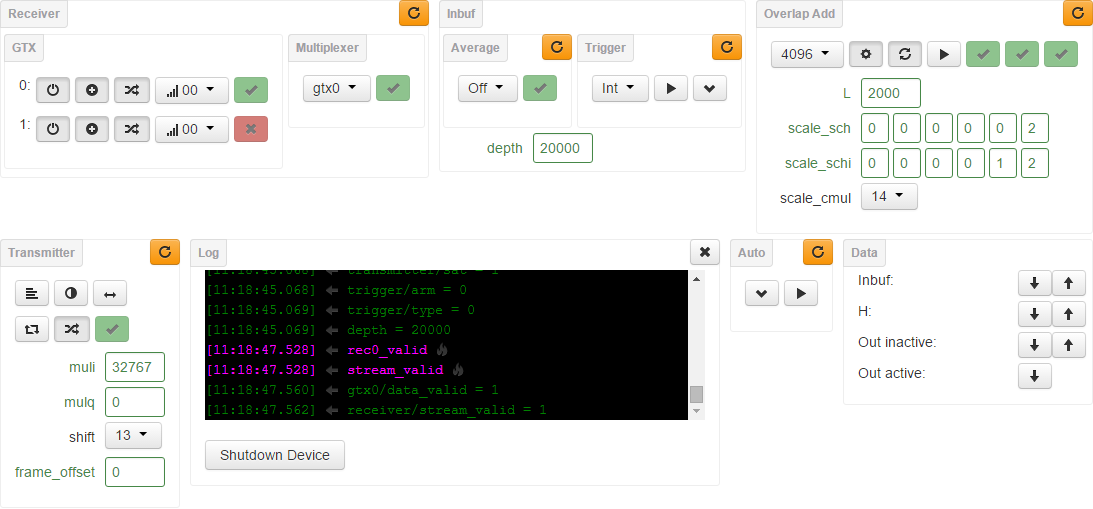
\includegraphics[width=\textwidth]{webinterface}
    \caption{Screen shot of the web interface}
    \label{fig:webinterface}
\end{figure}

The Matlab communication protocol consists of two different protocols. It is not
possible to use asynchronous and synchronous network communication over a single
connection within Matlab. Therefore, a synchronous line based protocol was implemented.
One command can be transmitted per line and every line starts with a command, followed
by a space separated list of arguments. The commands are the same as in the \gls{json}
based protocol ({\ttfamily get}, {\ttfamily set}, {\ttfamily do}). Since this protocol is synchronous, the
{\ttfamily do} command waits for the appropriate interrupt before replying. The daemon replies
{\ttfamily OK} in the case of success or {\ttfamily ERROR} in case of an error (e.g. timeout). An example
command can be seen in \cref{src:text}. The additional commands {\ttfamily read} and {\ttfamily write}
implement interacting with the sample buffers. Both commands need the name of the target memory as
the first argument ({\ttfamily emce0} to {\ttfamily emce3}) and the number of bytes as the second
argument. The {\ttfamily write} command has to be followed by the specified number of bytes of raw data after the
newline. The {\ttfamily read} command provides the specified number of raw bytes instead of the {\ttfamily OK} reply.
The raw data is composed of \SI{16}{\bit} signed integers with big endian byte ordering. This protocol implementation
can be reached via the \gls{tcp} port {\ttfamily 8000}.

\begin{lstlisting}[language={},float=htb,caption={Example line to set $\gls{L}=2000$ with the text based protocol},label=src:text,basicstyle=\hack\scriptsize]
set core/L 2000
\end{lstlisting}

Additionally to this protocol a second asynchronous
protocol was implemented that allows to be notified about interrupts. Any input to
this protocol is ignored. Interrupts are reported via this protocol with the name of the interrupt
followed by a newline. The asynchronous protocol listens on \gls{tcp} port {\ttfamily 8001}.

This daemon is started automatically during the \gls{os} boot sequence. The \gls{json}- and
text based protocol both provide an additional shutdown command that allows shutting
down the \gls{os}. The \gls{os} should always be shut down before switching off the \gls{fpga}
to prevent file system corruption. The source code for the daemon can be found in \cref{sec:sources}.

% ---------------------------------------------------------------------------

\section{Matlab Algorithms}
\label{sec:matlab}
\lstset{language=Matlab}

The text based protocol described in \cref{sec:daemon} was implemented in a set of
Matlab classes to ease controlling the hardware. These Matlab classes depict the
same naming scheme as the \device{sysfs} interface with a dot instead of a slash
as the path separator. The sample buffers can be accessed via the properties
\lstinline+inbuf+ for \device{inbuf}, \lstinline+H+ for \device{H},
\lstinline+out_inactive+ for inactive \device{outbuf}, and \lstinline+out_active+
for active \device{outbuf} (see \cref{sec:digital_processing}). Those dependent properties automatically convert
the raw data to complex vectors and vice versa. The interrupts are exposed via
Matlab events. All the classes are fully documented with Matlab comments and
can be found in \cref{sec:sources}. A description of all the properties can
be found in \cref{sec:registers}. An example usage can be seen in \cref{src:mdriver}.

\begin{lstlisting}[float=htb,caption={Example usage of the Matlab driver for the hardware},label=src:mdriver,basicstyle=\hack\scriptsize,texcl=true]
ml507 = ML507.ML507(); %\upshape instantiate the class

ml507.depth = 20000; %\upshape set signal period $\gls{N} = \num{20000}$
ml507.transmitter.mul = 32767; %\upshape set $\glsdisp{GammaL}{\Gamma_{L,set}} = \num{32767}$
ml507.transmitter.shift = 5; %\upshape set output multiplier shift to 5
ml507.core.n = 4096; %\upshape set $\gls{nfft} = \num{4096}$
ml507.core.L = 2000; %\upshape set $L = \num{2000}$
ml507.core.scale_sch(1:6) = [2 0 0 0 0 0]; %\upshape schaling schedule for \gls{fft}
ml507.core.scale_schi(1:6) = [2 1 0 0 0 0]; %\upshape schaling schedule for inverse \gls{fft}
ml507.core.scale_cmul = 1; %\upshape complex multiplier scaling
ml507.core.iq = 1; %\upshape enable iq decode
ml507.core.circular = 1; %\upshape enable circular convolution
ml507.transmitter.resync(); %\upshape resync transmitter to set signal period
ml507.trigger.arm(); %\upshape arm trigger
ml507.trigger.fire(); %\upshape fire trigger
\end{lstlisting}

Utilizing these classes the one port \gls{vna} as described in \cref{sec:vna}
was implemented in a Matlab script. A description of this script can be found
in \cref{sec:mvna}. Additional reflections caused by the measurement setup and the \gls{dut} cause
the setup to exhibit a different \gls{GammaL} than was set by
$\glsdisp{GammaL}{\Gamma_{L,set}}$. These imperfections can be compensated with an error
box as has been done for the one port \gls{vna} (see \cref{sec:vna}).
Since highly non-linear \gls{dut} can experience load-dependent
$\gls{S}[_{22}]$, this approach could prove futile. Therefore, an iterative target algorithm
was developed to find the correct $\glsdisp{GammaL}{\Gamma_{L,set}}$ needed
to achieve a specific $\glsdisp{GammaL}{\Gamma_{L,target}}$. This algorithm
is described in \cref{sec:target}. Using this target algorithm the
filter calibration script, described in \cref{sec:filtercal}, was developed.

% ---------------------------------------------------------------------------

\subsection{One Port \glsentryshort{vna}}
\label{sec:mvna}

The one port \gls{vna} as described in \cref{sec:vna} determines the reflection
coefficient \gls{GammaL} by measuring the magnitude and the phase of the incident
and reflected power waves. This measurement has to be corrected for systematic
errors with the error box described in \cref{sec:vna}. To be able to use
this error box additional calibration measurements have to be carried out
beforehand.

The sampled data and the timebase from the oscilloscope were acquired using the
Instrument Control Toolbox in Matlab. To extract the magnitude and the phase
with high accuracy for specific frequencies the samples were multiplied with
a flat top window (see \cref{sec:vna}). Next, this modified data was transformed
with the \gls{fft} into the frequency domain. After that the reflection coefficient
was calculated by dividing the transformed data from the incident and the reflected
power wave at the indices corresponding to the desired frequencies. The Matlab
function implementing this functionality can be seen in \cref{src:manyrho}.

\begin{lstlisting}[float=htb,caption={Function for calculating $\frac{\gls{a}}{\gls{b}}$ from sampled data at multiple frequencies},label=src:manyrho,basicstyle=\hack\scriptsize]
function [rho, A, B] = manyRho(xincrement, a, b, freqs)
    A = fft(a.*flattopwin(length(a), 'periodic'));
    B = fft(b.*flattopwin(length(b), 'periodic'));

    df = 1/xincrement/length(A);
    freqs = floor(freqs./df)+1;

    A = A(freqs);
    B = B(freqs);

    rho = A./B;
end
\end{lstlisting}

The calibration of the error box was realized by measuring three different targets
at multiple frequencies. In order to enable measurements with the possible
frequency resolution of the oscilloscope, the calibration measurements were
linearly interpolated. A Rohde \& Schwarz Z132 (female) calibration kit was used
for this calibration. To be able to calculate the impedance values of the
calibration kit the Matlab function \lstinline+calcZ132+ was developed. This function
calculates the short, match, and open impedance for a given frequency according to
the data sheet \cite{zv-z132}. The Matlab function called \lstinline+calcErrorBoxM+ was
generated with a Mathematica notebook which was used to solve the equations
derived from the error box in \cref{sec:vna}. With the impedance values from
the calibration kit and the calibration measurement values this function calculates
the \glspl{sparam} of the error box.

The developed function \lstinline+calcGl+ is able to calculate a corrected \gls{GammaL}
with these \glspl{sparam} and a reflection coefficient calculated with \lstinline+manyRho+
from acquired samples. The described functions and the example script \lstinline+measureVNA+
can be found in \cref{sec:sources}. This example script is split into four parts. The
first part initializes the used instruments, the second part carries out the
calibration measurements, and the third part implements the interpolation
and error box calculations. The fourth part contains the measurement used to generate
the verification data for \cref{sec:vna_verify}.

% ---------------------------------------------------------------------------

\subsection{Target Algorithm}
\label{sec:target}

As described above, the resulting \gls{GammaL} of the complete setup is
influenced by additional reflections resulting from imperfections in the
measurement setup. Furthermore, highly non-linear \gls{dut}
can experience load-dependent $\gls{S}[_{22}]$ which influence
the resulting \gls{GammaL} additionally. Therefore, the following iterative
target algorithm was developed.

The iterative target algorithm used in this work makes the following steps:
\begin{enumerate}
    \item Start at arbitrary start point by setting $\glsdisp{GammaL}{\Gamma_{L,set}}$.
    \item Measure the resulting \gls{GammaL}.
    \item If $\abs{\Gamma_L - \Gamma_{L,target}} < accuracy$ then the algorithm is done. The
        accuracy used in this work was a magnitude difference \num{< 1e-3} and a phase difference \SI{<0.25}{\degree}.
    \item Scale $\glsdisp{GammaL}{\Gamma_{L,set}}$ according to $\frac{\Gamma_{L,target}}{\Gamma_L}$.
    \item Pause to compensate for lag time introduced by the digital signal processing chain.
    \item Repeat from step 2.
\end{enumerate}

\begin{figure}[htb]
    \centering
    \begin{tikzpicture}
        \begin{scope}[shift={(0,4.5)}]
            \foreach \x in {0,...,11}
            {
                \begin{scope}[shift={($\x*(0.8,0)-(5,0)$)}]
                    \fill [YlOrRd-3-1] (0,0)   |- (0.2,1) node[coordinate] (acquire-n-\x) {} -- (0.2,0) node[coordinate] (acquire-s-\x) {} -- cycle;
                    \fill [YlOrRd-3-2] (0.2,0) |- (0.6,1) node[coordinate] (filter-n-\x) {} -- (0.6,0) node[coordinate] (filter-s-\x) {} -- cycle;
                    \fill [YlOrRd-3-3] (0.6,0) |- (0.8,1) node[coordinate] (switch-n-\x) {}  -- (0.8,0) node[coordinate] (switch-s-\x)  {} -- cycle;
                \end{scope}
            }
            \draw [-latex] (-5,0) --  (5,0) node[anchor=west,font=\tiny] {time};
            \draw (-5,0.5) node[anchor=east,font={}] (phase) {\gls{fpga} Phase};
        \end{scope}
            \begin{scope}
                \clip (-5,-1) rectangle (4.6,2);
                \node[coordinate] at (-4.7,0) (measure-start) {};
                \foreach \x in {0,1}
                {
                    \begin{scope}[shift={($\x*(5.7,0)-(4.7,0)$)}]
                        \fill[Set2-4-1] (0,0)   |- (1.4,1) node[coordinate] (measure-n-\x) {} -- (1.4,0) node[coordinate] (measure-s-\x) {} -- cycle;
                        \fill[Set2-4-2] (1.4,0) |- (1.5,1) node[coordinate] (compute-n-\x) {} -- (1.5,0) node[coordinate] (compute-s-\x) {} -- cycle;
                        \fill[Set2-4-3] (1.5,0) |- (1.6,1) node[coordinate] (set-n-\x) {}     -- (1.6,0) node[coordinate] (set-s-\x) {}     -- cycle;
                        \fill[Set2-4-4] (1.6,0) |- (5.7,1) node[coordinate] (pause-n-\x) {}   -- (5.7,0) node[coordinate] (pause-s-\x) {}   -- cycle;
                    \end{scope}
                }
                \fill[yellow!33] (-5,0) rectangle (-4.7,1);
            \end{scope}

            \draw [-latex] (-5,0) --  (5,0) node[anchor=west,font=\tiny] {time};
            \draw (-5,0.5) node[anchor=east,font={}] (target) {Algorithm Phase};
        \begin{scope}[shift={(0,3)}]
            \draw (-5,0.5) node[anchor=east,font={}] (b2) {$\gls{b}[_2]$};
            \fill[green] (-5,0) rectangle ($(set-n-0 |- 0,1)+(0.2,0)$) node[coordinate] (b-n-1) {};
            \fill[red!33] (b-n-1 |- 0,0) node[coordinate] (b-s-1) {} rectangle ($(switch-s-3 |- 0,1)+(0.1,0)$) node[coordinate] (b-n-2) {};
            \fill[red!66] (b-n-2 |- 0,0) node[coordinate] (b-s-2) {} rectangle ($(switch-s-5 |- 0,1)+(0.1,0)$) node[coordinate] (b-n-3) {};
            \fill[red]    (b-n-3 |- 0,0) node[coordinate] (b-s-3) {} rectangle ($(set-n-1 |- 0,1)+(0.2,0)$) node[coordinate] (b-n-4) {};
            \fill[blue!33](b-n-4 |- 0,0) node[coordinate] (b-s-4) {} rectangle ($(switch-s-10 |- 0,1)+(0.1,0)$) node[coordinate] (b-n-5) {};
            \fill[blue!66](b-n-5 |- 0,0) node[coordinate] (b-s-5) {} rectangle (4.6,1);
            \draw [-latex] (-5,0) --  (5,0) node[anchor=west,font=\tiny] {time};
        \end{scope}
        \begin{scope}[shift={(0,1.5)}]
            \draw (-5,0.5) node[anchor=east,font={}] (a2) {$\gls{a}[_2]$};
            \fill[green] (-5,0) rectangle ($(set-n-0 |- 0,1)+(0.1,0)$) node[coordinate] (a-n-1) {};
            \fill[red!33] (a-n-1 |- 0,0) node[coordinate] (a-s-1) {} rectangle (switch-s-3 |- 0,1) node[coordinate] (a-n-2) {};
            \fill[red!66] (a-n-2 |- 0,0) node[coordinate] (a-s-2) {} rectangle (switch-s-5 |- 0,1) node[coordinate] (a-n-3) {};
            \fill[red]    (a-n-3 |- 0,0) node[coordinate] (a-s-3) {} rectangle ($(set-n-1 |- 0,1)+(0.1,0)$) node[coordinate] (a-n-4) {};
            \fill[blue!33](a-n-4 |- 0,0) node[coordinate] (a-s-4) {} rectangle (switch-s-10 |- 0,1) node[coordinate] (a-n-5) {};
            \fill[blue!66](a-n-5 |- 0,0) node[coordinate] (a-s-5) {} rectangle (4.6,1);
            \draw [-latex] (-5,0) --  (5,0) node[anchor=west,font=\tiny] {time};
        \end{scope}
        \begin{scope}[-latex]
            \draw (set-n-0) -- (a-s-1) node[midway,right,font=\tiny] {$\glsdisp{GammaL}{\Gamma_{L,set,0}}$};
            \draw (set-n-1) -- (a-s-4) node[midway,right,font=\tiny] {$\glsdisp{GammaL}{\Gamma_{L,set,1}}$};
            \foreach \x in {1,...,5}
            {
                \draw (a-n-\x) -- (b-s-\x);
            }
            \draw (b-n-1 -| switch-s-2) -- (switch-s-2);
            \draw (b-n-1 -| switch-s-4) -- (switch-s-4);
            \draw (b-n-1 -| switch-s-9) -- (switch-s-9);
            \draw (switch-n-3) to[bend right=10] (a-s-2);
            \draw (switch-n-5) to[bend right=10] (a-s-3);
            \draw (switch-n-10) to[bend right=10] (a-s-5);
            \draw (measure-start |- b-n-1) to[bend right=10] (measure-start);
            \draw (measure-start |- a-n-1) to[bend left=10] (measure-start);
            \draw (pause-s-0 |- b-n-1) to[bend right=10] (pause-s-0);
            \draw (pause-s-0 |- a-n-1) to[bend left=10] (pause-s-0);
        \end{scope}

        \draw ($(switch-n-2)!.5!(acquire-n-3)$) -- ++(-1,0.5) node[draw,fill=YlOrRd-3-1] {Acquire};
        \draw ($(acquire-n-3)!.5!(filter-n-3)$) -- ++(0,1.2) node[draw,fill=YlOrRd-3-2] {Filter};
        \draw ($(filter-n-3)!.5!(switch-n-3)$) -- ++(1,0.5) node[draw,fill=YlOrRd-3-3] {Switch};

        \draw ($(measure-start)!.5!(measure-s-0)$) -- ++(-1,-0.5) node[draw,fill=Set2-4-1] {Measure \gls{GammaL}};
        \draw ($(measure-s-0)!.5!(compute-s-0)$) -- ++(-.7,-1.5) node[draw,fill=Set2-4-2] {Calculate new $\glsdisp{GammaL}{\Gamma_{L,set}}$};
        \draw ($(compute-s-0)!.5!(set-s-0)$) -- ++(3,-1.5) node[draw,fill=Set2-4-3] {Set new $\glsdisp{GammaL}{\Gamma_{L,set}}$};
        \draw ($(set-s-0)!.5!(pause-s-0)$) -- ++(1,-0.5) node[draw,fill=Set2-4-4] {Pause};
    \end{tikzpicture}
    \caption[Visualization of the different phases of the \glsentryshort{fpga} implementation and target algorithm over time]{Visualization of the different phases of the \glsentryshort{fpga} implementation and target algorithm over time (not to scale)}
    \label{fig:phases}
\end{figure}

The pause is needed, because the digital signal processing chain experiences
lag times up to \SI{1}{\milli\second}. Since this algorithm and the digital
signal processing chain run completely independent, the algorithm can
experience stability issues if the pause of the algorithm is too short. A
visualization of the different phases of the digital signal processing chain
and the algorithm can be seen in \cref{fig:phases}. In this visualisation it
can be seen that the algorithm starts by
measuring \gls{GammaL}. After the new $\glsdisp{GammaL}{\Gamma_{L,set}}$ is
set, the wave $\gls{a}[_2]$ is modified immediately, which in turn results in
a new $\gls{b}[_2]$. After the next acquire, filter, and switch cycle of the
digital signal processing chain, a new wave $\gls{a}[_2]$ is generated, which
results again in a new $\gls{b}[_2]$. If the pause of iterative algorithm
is too short, then the next step will be based on a wrong \gls{GammaL}
measurement, which can lead to a high number of algorithm steps.

Preliminary tests showed that this iterative target algorithm is capable
of reaching multiple specific $\glsdisp{GammaL}{\Gamma_{L,target}}$. Therefore,
the algorithm is capable of compensating the reflections introduced by
the measurement setup. These are caused by connectors and mismatches between
the components. The iterative target algorithm also
worked after additional reflections have been introduced intentionally in the
measurement setup. A more detailed verification of this algorithm can be found
in \cref{sec:iterative}.

The iterative target algorithm was implement in the Matlab function \lstinline+findTarget+.
The needed
arguments are a \lstinline+ML507+ object for controlling the signal processing
chain, the target, a function handle to a function implementing the
\gls{GammaL}-measurement, and the pause time. Additionally, a start point
can be specified. The \lstinline+findTarget+ function returns upon algorithm termination the actual
\gls{GammaL} and the needed $\glsdisp{GammaL}{\Gamma_{L,set}}$. Additionally, the complete
trajectory consisting of every reached \gls{GammaL}, including start and stop point,
is returned.

% ---------------------------------------------------------------------------

\subsection{Filter Calibration}
\label{sec:filtercal}

The digital filter in the signal processing chain is needed to
synthesize a constant \gls{GammaL} over a wide frequency range. This
filter is required to compensate the group delay caused by the measurement
setup and cabling needed for to be able to reach the \gls{dut}. Furthermore,
it is able to compensate the frequency responses of the components used
in the measurement setup.

Calibrating this filter was carried out by measuring the needed
$\glsdisp{GammaL}{\Gamma_{L,set}}$ for a specific calibration point over
the required frequency range. This calibration data was linearly interpolated to
cover every frequency point of the digital filter. Since the measured values
experience very high phase differences, the data was split into magnitude and
unwrapped phase for the interpolation. After interpolation, the
$\glsdisp{GammaL}{\Gamma_{L,set}}$ values were added to the filter by multiplying
them with the transfer function. An example of the resulting transfer function
can be seen in \cref{sec:filter}.

An example script named \lstinline+filterCalibration+ is provided in
\cref{sec:sources} which acquires a filter calibration for the points
$1$, $-1$, $0.5\angle\SI{135}{\degree}$ and $0.5\angle\SI{-45}{\degree}$.
Additionally it calculates filters for the mean of the measurements $1$ and $-1$,
and $0.5\angle\SI{135}{\degree}$ and $0.5\angle\SI{-45}{\degree}$. After these
calculations the script performs verification measurements for the different
filter calibrations. The results of these measurements can be found in \cref{sec:filter}.

% ===========================================================================

\chapter{Verification of the Measurement System}
\label{chap:verification}
\lstset{language=matlab}

The implemented \gls{elp} design was tested with the setup presented in
\cref{fig:test_setup} at a center frequency $\gls{f0}$ of \SI{900}{\mega\hertz}. This test setup consists of the three parts
which have been described in \cref{chap:measurement_system}. As mentioned in
\cref{sec:analog}, instead of a circulator, the directional coupler
\device{dir2} in combination with attenuator \device{att1} was used.
Furthermore, since during verification only waves synthesized inside
the specified bandwidth of \SI{20}{\mega\hertz} were used, the low-pass filter \device{lp2}
was used instead of a bandpass filter. A detailed list of used
equipment can be seen in \cref{sec:instruments}.

\begin{figure}[htb]
    \centering
    \resizebox{\linewidth}{!}{
    \begin{tikzpicture}
        \pgfdeclarelayer{foreground}
        \pgfsetlayers{background,main,foreground}
        \tikzpicturedependsonfile{rfsymbols.tex}
        \tikzstyle{every node}=[font=\footnotesize]
        \draw node[dut] (dut) {}
              node[dircoupler,right=2 of dut,label=below:dir1,label={[font=\tiny]above:\SI{-16}{\deci\bel}}] (dirvna) {}
              node[oscilloscope,above=of dirvna.A2,anchor=A1] (oszivna) {}
              node[dircouplera,right=of dirvna,label=below:dir2,label={[font=\tiny]above:\SI{-16}{\deci\bel}}] (dircirc) {}

              node[coordinate,above=2.5 of dircirc] (uppernode) {}

              node[attenuator,right=of dircirc,label=above:att1,label={[font=\tiny]below:\SI{10}{\deci\bel}}] (att) {}
              node[amplifier,right=of att,label=above:amp1] (amp) {}
              node[mixer,right=of amp,label=above:mix3] (upmix) {}
              node[lowpass,right=of upmix,label=above:lp1] (antialias) {}
              node[adc,right=of antialias,label=above:dac1] (dac) {}

              (uppernode -| upmix) node[mixer,label=below:mix1] (downmix) {}
              node[lowpass,right=of downmix,label=below:lp2,label={[font=\tiny]above:\SI{90}{\mega\hertz}}] (bp) {}
              node[adc,right=of bp,label=below:adc1] (adc) {}
              node[empty,right=of adc,label=below:buffer1] (inbuf) {}
              node[mixer,right=of inbuf] (shift) {}
              node[rotate=90,anchor=north] at (shift.east) {mix2}

              (dac -| inbuf) node[mixer,label=above:mul1] (mul) {}
              node[empty,right=of mul] (outbuf) {}
              node[rotate=90,anchor=north] at (outbuf.east) (buffer2) {buffer2}

              ($(shift)!.5!(outbuf)$) node[allpass,rotate=90] (H) {}
              node[rotate=90,anchor=north] at (H.south) {fir1}

              node[source,above=of downmix.center,scale=0.7] (downsource) {}
              node[rotate=90,anchor=south,font=\tiny] at (downsource.west) {$\SI{830}{\mega\hertz}$}
              node[rotate=90,anchor=north] at (downsource.east) {lo1}
              node[source,above=of adc.center,scale=0.7] (sample) {}
              node[rotate=90,anchor=south,font=\tiny] at (sample.west) {$\SI{100}{\mega\hertz}$}
              node[rotate=90,anchor=north] at (sample.east) {lo2}
              node[source,above=of shift.center,scale=0.7] (shiftsource) {}
              node[rotate=90,anchor=south,font=\tiny] at (shiftsource.west) {$\SI{30}{\mega\hertz}$}
              node[rotate=90,anchor=north] at (shiftsource.east) {lo3}
              node[source,below=of upmix.center,scale=0.7] (upsource) {}
              node[rotate=90,anchor=south,font=\tiny] at (upsource.west) {$\SI{900}{\mega\hertz}$}
              node[rotate=90,anchor=north] at (upsource.east) {lo4}
              node[below=of mul.center,fill=white] (gamma) {$\glsdisp{GammaL}{\Gamma_{L,set}}$};

        \draw ($(dut)!.5!(dirvna)$) node[coordinate] (plane) {};

        { [rounded corners=2pt]
            \draw (dut) -- (dirvna) -- (dircirc.A1);
            \draw [-latex] (dircirc.A2) |- (downmix) node[above,near end] {$\gls{b}[_2]$};
            \draw (dirvna.A2) -- (oszivna.A1);
            \draw (dirvna.B2) |- ($(dirvna.B2)!.7!(oszivna.A2)$) node[coordinate] (oszimiddle) {} -| (oszivna.A2);
            \draw [-latex] (att) -- (dircirc.B1) node[midway,above] {$\gls{a}[_2]$};
        }
        { [-latex]
            \draw (downsource) -- (downmix);
            \draw (sample) -- (adc);
            \draw [double] (shiftsource) -- (shift);
            \draw [double] (gamma) -- (mul);
            \draw (upsource) -- (upmix);
        }
        { [latex-,dashed,every node/.style={font=\footnotesize}]
            \foreach \device in {downsource,sample} {
                \draw (\device) -- ++(0,1) node[anchor=south] {\SI{10}{\mega\hertz} ref};
            }
            \draw ([xshift=0.5cm]oszivna.north) -- ++(0,0.5) node[fill=white,anchor=south] {\SI{10}{\mega\hertz} ref};
        }
        { [start chain,every on chain/.style={join=by -latex}]
            \chainin (downmix);
            \chainin (bp);
            \chainin (adc);
            \chainin (inbuf);
            \chainin (shift);
            { [every on chain/.style={join=by {double,-latex}}]
                \chainin (H);
                \chainin (outbuf);
                \chainin (mul);
                \chainin (dac);
                \chainin (antialias);
                \chainin (upmix);
            }
            \chainin (amp);
            \chainin (att);
        }
        { [on background layer,every path/.style={dotted,decorate,decoration=random steps,segment length=2mm}]
            \draw ($(dirvna.B1)!.5!(dircirc.A1) + (0,5.5)$) -- ++(0,-8.5) node[coordinate] (leftsplit) {};
            \draw ($(adc.east)!.5!(mul.west) + (0,4)$) -- ++(0,-8.5) node[coordinate] (rightsplit) {};
        }

        \draw (leftsplit) node[anchor=base east] {One Port \gls{vna}}
              (leftsplit) node[anchor=base west] {Analog}
              (rightsplit) node[anchor=base west] {Digital}
              (rightsplit) node[anchor=base east] {Analog};

%        \draw [-latex] ($(dirvna.A2) + (-0.2,0.1)$) -- node[base left] {$b_1$} ($(oszivna.A1 |- oszimiddle) - (0.2,0.1)$);
%        \begin{pgfonlayer}{foreground}
%            \draw [-latex] ($(dirvna.B2) + (0.2,0.1)$) -- ($(oszimiddle -| dirvna.B2) + (0.2,-0.1)$);
%        \end{pgfonlayer}
%        \draw ($(oszimiddle -| dirvna.B2) + (0.2,-0.1)$) node[base right,fill=white] {$a_1$};

        \draw [dashed] ($(plane) + (0,5.5)$) node[anchor=south] {Load Reference Plane} -- ($(plane) - (0,3)$);

        \draw [latex-] ($(plane) + (0,1.5)$) -- ++(-0.5,0) node[anchor=east] {$\gls{ZL}$};

        \draw [-latex] ($(plane) + (0.25,-1.5)$) node[anchor=west] {$\gls{a}[_2]$}-- ++(-0.5,0);
        \draw [latex-] ($(plane) + (0.25,-2)$) node[anchor=west] {$\gls{b}[_2]$}-- ++(-0.5,0);
        \draw [latex-] ($(plane) + (0,-2.5)$) -- ++(-0.5,0) node[anchor=east] {$\gls{GammaL}$};
        \node [draw,fit=(amp) (dac) (upsource),rounded corners=4pt,inner xsep=6pt,inner ysep=14pt,label={above:Vector Signal Generator}] (sig) {};
        \draw [-latex,dashed] ([xshift=-2cm]sig.south) -- ++(0,-0.5) node[anchor=north] {\SI{10}{\mega\hertz} ref};
        \node [draw,fit=(gamma) (outbuf) (inbuf) (shiftsource) (buffer2),rounded corners=4pt,inner xsep=6pt,inner ysep=14pt,label={above:\gls{fpga}}] (fpga) {};

        {[densely dashdotdotted,latex-latex]
            \draw (fpga.east) -- ++(1,0) node [anchor=west] {\gls{pc}};
            \draw (sig.south) -- ++(0,-0.5) node [anchor=north] {\gls{pc}};
            \draw ([xshift=-0.5cm]oszivna.north) -- ++(0,1) node [anchor=south] {\gls{pc}};
        }

        \draw [decorate,decoration={brace,mirror,amplitude=5pt}] ([yshift=-6pt]leftsplit) -- (\currentcoordinate -| fpga.south east) node[midway,below,yshift=-6pt] {reflection generation};
    \end{tikzpicture}
    }
    \caption{Measurement system verification test setup}
    \label{fig:test_setup}
\end{figure}

The overall setup consists of two independent systems. The one port \gls{vna} and
the reflection generation consisting of the analog and the digital part. The
one port \gls{vna} is needed to measure the current $\gls{GammaL}$ (see
\cref{sec:vna}). Verification of this part can be found in \cref{sec:vna_verify}. As
described in \cref{sec:analog}, the analog part is responsible for separating the
incident wave $\gls{b}[_2]$, converting it to \gls{if}, and digitally sampling the signal.
Furthermore it handles digital-to-analog conversion, up-conversion to \gls{rf} and
feeding back the reflected wave $\gls{a}[_2]$ to the \gls{dut}. The digital part as described
in \cref{sec:digital} handles filtering the signal to enable broadband reflection
synthesis and applying the reflection coefficient $\glsdisp{GammaL}{\Gamma_{L,set}}$. Since analog and
digital part can't be verified separately, verification of the combined reflection
generation part can be found in \cref{sec:reflection}. During these measurements,
a noticeable phase drift was observed, and, therefore, an additional measurement was
acquired, as seen in \cref{sec:drift}, to verify the origin
of this phase drift.

% ---------------------------------------------------------------------------

\section{One Port \glsentryshort{vna} Verification}
\label{sec:vna_verify}

For the calibration and verification of the one port \gls{vna}, the modulator of
the vector signal generator was turned off. Stepping through the frequency range
was achieved by stepping the local oscillator \device{lo4} (see \cref{fig:test_setup}).
This allowed for easier test automation since only the vector signal generator had to
be controlled. The vector signal generator was set to an output power of \SI{0}{\deci\belm}
which results in about \SI{-10}{\deci\belm} at the load reference plane (see \cref{fig:test_setup}). A ZV-Z132 (female) calibration kit from Rohde \& Schwarz was used for the calibration
setup in place of the \gls{dut}. Since the calibration is only valid for a single frequency, the full
calibration measurements were acquired for 21 $\Delta{}\gls{f}$-aligned points within a
\SI{25}{\mega\hertz} range at a center frequency of \SI{900}{\mega\hertz}. This
was achieved by connecting the appropriate port of the calibration kit and acquiring
$\glsdisp{GammaL}{\Gamma_{L,f}}$ values for every frequency point. After the measurement, the different $\glsdisp{GammaL}{\Gamma_{L,f}}$ were linearly
interpolated at every $\Delta{}\gls{f}$ bin. Finally, the \glspl{sparam} of
the error box (see \cref{sec:vna}) were pre-calculated for every bin utilizing the values
from the data sheet of the calibration kit\cite{zv-z132}.

For the verification of the calibration, a stub tuner from Maury Microwave was tuned to a specific position and
then measured utilizing the one port \gls{vna} in this work. Measurements were acquired over
the whole \SI{25}{\mega\hertz} bandwidth at the calibrated points. Additional measurements
were acquired at an offset of $\frac{1}{2}\Delta{}\gls{f}$, to test the performance
of the chosen window function. The performance of the interpolation was further tested by
measurements between the calibrated points. To verify the $\gls{GammaL}$, which was measured using the
above described setup, those measurements were compared to a measurement acquired using a
commercially available \gls{vna}. The \gls{vna} used for verification was an Agilent Technologies E8364A,
calibrated with an Agilent Technologies N4433A calibration kit (see \cref{sec:instruments}). \gls{vna}
settings used were \SI{-10}{\deci\belm} test port power, \SI{35}{\kilo\hertz} \gls{if} bandwidth, and
\num{1601} measurement points.

Every point was measured 100 times to be able to quantify the non systematic errors. With those
$N$ observations of every point, the measured samples $x$, and the mean of the measured samples
$\mean{x}$, the corrected sample standard deviation $s$ was calculated according to \cref{eq:std}.
With the sample standard deviation $s$ the standard error $S\!E$ was calculated according to \cref{eq:stderr}.

\begin{align}
    \label{eq:std} s &= \sqrt{\frac{1}{N-1} \sum^N_{i=1} (x_i - \mean{x})^2} \\
    \label{eq:stderr} S\!E &= \frac{s}{\sqrt{N}}
\end{align}

The standard error and the difference to the results from the Agilent \gls{vna} roughly stay the
same over the complete \SI{25}{\mega\hertz} range. There is also no noticeable difference between
the three different types of points. Thus, the linear interpolation and the chosen window function
seem to be appropriate for this type of measurement. Since there are only passive parts involved
in the one port \gls{vna}, it should also be possible to use less calibration points to achieve a
faster calibration. The measurement result of three exemplary points can be seen in \cref{tab:vna}.

\begin{table}[htb]
    \centering
    \begin{subtable}[b]{\linewidth}
        \centering
        \begin{tabular}{
            S[table-format=3.3]
            l
            S[table-format=3.4e1]
            S[table-format=2.1e1]
            S[table-format=1.1e1]}
            \toprule
            \multicolumn{2}{c}{{\textbf{frequency}}} & {\textbf{mean}} & {\textbf{standard error}} & {\textbf{$\Delta$\gls{vna}}} \\
            {\si{\mega\hertz}} &  & {1} & {1} & {1} \\
            \midrule
            887.5   & (cal)                          & 581.0232e-3 & 37.6e-6 & 2.1e-3 \\
            887.505 & ($\frac{1}{2}\Delta{}\gls{f}$) & 581.0589e-3 & 38.2e-6 & 2.2e-3 \\
            888.095 &(between cal)                   & 582.3070e-3 & 36.6e-6 & 2.1e-3 \\%\midrule
            \bottomrule
        \end{tabular}
        \caption{Magnitude}
    \end{subtable}\vspace{1em}\\
    \begin{subtable}[b]{\linewidth}
        \centering
        \begin{tabular}{
            S[table-format=3.3]
            l
            S[table-format=+3.4]
            S[table-format=1.1e1]
            S[table-format=1.1]}
            \toprule
            \multicolumn{2}{c}{{\textbf{frequency}}} & {\textbf{mean}} & {\textbf{standard error}} & {\textbf{$\Delta$\gls{vna}}} \\
            {\si{\mega\hertz}} &  & {\si{\degree}} & {\si{\degree}} & {\si{\degree}} \\
            \midrule
            887.5   & (cal)                          & -157.5029 & 8.7e-3 & 2.2 \\
            887.505 & ($\frac{1}{2}\Delta{}\gls{f}$) & -157.4787 & 8.1e-3 & 2.3 \\
            888.095 &(between cal)                   & -157.7972 & 9.7e-3 & 2.3 \\
            \bottomrule
        \end{tabular}
        \caption{Angle}
    \end{subtable}
    \caption{Measured reflection coefficient with standard error and difference to Agilent \glsentryshort{vna}}
    \label{tab:vna}
\end{table}

The setup of the one port \gls{vna} consists of an oscilloscope and only passive components.
Therefore, the standard error notably depends on the performance of the oscilloscope. It is
mainly caused by the \glspl{adc} contained in the oscilloscope and imperfections in the
triggering and sampling. This also means that these results are only valid for the
used oscilloscope in this work.

The difference to the results from the Agilent \gls{vna} are mainly caused by the
used calibration kit. This is caused by the performance of the error box as described in
\cref{sec:vna} which was used to correct the systematic errors. The calibration of the error
box depends only on measurements of the calibration standard. Therefore, the performance can
be increased with a better calibration kit or by additional calibration measurements.

Further care should be taken to always ensure a strong enough signal power at the
oscilloscope \glspl{adc}. According to \cite{Oppenheim} the \gls{snr} caused by quantization
noise of \gls{adc} depends on the bit width and the amplitude. Therefore, small signals cause
a low \gls{snr}. A small \gls{GammaL} value implies a small reflected wave and therefore a
lower \gls{snr}. Therefore, the resolution decreases for small \gls{GammaL}. This can
be compensated with averaging which would increase the effective bit width at the cost
of longer measurement times \cite{ad_mt004}.

% ---------------------------------------------------------------------------

\section{Reflection Generation Verification}
\label{sec:reflection}

The reflection measurements were carried out using a test setup as displayed in \cref{fig:test_setup}.
Here an Agilent \gls{vna} was connected instead of the \gls{dut} to verify the synthesized reflection
coefficients. Furthermore, the Agilent \gls{vna} was synchronized to the setup using the same
\SI{10}{\mega\hertz} reference in order to be able to synthesize the needed phase coherent
signals for the test setup. This allowed verifying the synthesized $\gls{GammaL}$, and
calibrating the \gls{fir} filter \device{fir1} more accurately, than using the built
in one port \gls{vna}.

All the reflection generation verification measurements used \num{20000} samples as signal period \gls{N},
an overlap add block size \gls{L} of \num{2000}, and an \gls{fft} width $\gls{nfft}$ of \num{4096} (see
\cref{fig:overlap_add}). The filter \device{fir1} was preloaded with the
impulse response of a low pass filter with a cut off frequency of \SI{25}{\mega\hertz} to
filter out the aliases (see \cref{sec:digital}). For the duration of these measurements,
the \gls{fpga} implementation was switched to automatic mode which emulates continuous
signal processing (see \cref{sec:auto}). Changes at the input of the digital part propagate
with a lag time of about \SI{1}{\milli\second} to the output using automatic mode and the
above mentioned signal processing configuration.

The reflection generation consists of two tasks. First, the iterative target algorithm
described in \cref{sec:matlab} is needed, to synthesize specific $\gls{GammaL}$.
The performance of this algorithm can be seen in \cref{sec:iterative}. Second, this
algorithm was then used for calibrating and verifying the filter \device{fir1}. Measurement
results for the verification measurements utilizing the previously calibrated filter can be seen in \cref{sec:filter}.

\subsection{Iterative Target Algorithm}
\label{sec:iterative}

The target algorithm is able to find the correct $\glsdisp{GammaL}{\Gamma_{L,set}}$
with a given $\glsdisp{GammaL}{\Gamma_{L,start}}$ in order to synthesize a given
$\glsdisp{GammaL}{\Gamma_{L,target}}$. It works by setting the current \gls{GammaL}
into relation with the given $\glsdisp{GammaL}{\Gamma_{L,target}}$ and scaling
$\glsdisp{GammaL}{\Gamma_{L,set}}$ accordingly (see \cref{sec:matlab}). This
iterative target algorithm is needed to be able reach a specific \gls{GammaL} even
with highly non-linear \gls{dut}. These \gls{dut} can exhibit load dependent
$\gls{S}[_{22}]$ which renders error box based approaches unsuitable.

As mentioned above, the digital reflection generation introduces a large latency
on the order of about \SI{1}{\milli\second}. Therefore a delay time of \SI{100}{\milli\second}
was used for the iterative algorithm (see \cref{sec:matlab}). This allows the system to settle
on a $\gls{GammaL}$ before continuing with the algorithm. If the wait time is too short,
the iterative target algorithm can start to cause stability issues and the completion time of the algorithm
actually increases while a long wait time increases the completion time. The high delay
time of \SI{100}{\milli\second} was chosen since the Matlab function \lstinline|pause| is
not capable of short delays and exhibits very high inaccuracy \cite{matlab_pause}.

\begin{figure}[htb]
    \begin{subfigure}[b]{.5\linewidth}
        \centering
        \begin{tikzpicture}[
            spy/.style={%
                draw,green,
                line width=0.5pt,
                circle,inner sep=0pt,
            },
            ]
            \def\spyviewersize{3cm}
            \def\spyonclipreduce{0.5pt}
            \def\spyfactorI{10}

            \def\pic#1#2{
                \begin{smithchart}[width=.9\linewidth,clip=false#1]
                    \addplot[blue,is smithchart cs] file {testdata/filter/1.0,0/trajectory10.data};
                    \addplot[purple,is smithchart cs,only marks,mark=x#2] file {testdata/filter/1.0,0/trajectory10.data};
                    \draw (cartesian cs:1,0) node[coordinate] (a) {}
                          (cartesian cs:-0.4,0.4) node[coordinate] (b) {};
                \end{smithchart}
            }
            \pic{}{}
            \coordinate (spy-on 1) at (a);
            \coordinate (spy-in 1) at (b);

            \node[spy,ultra thick,circular drop shadow,minimum size=\spyviewersize,fill=white,label={[inner sep=0pt,yshift=-5pt,fill=white,font=\footnotesize]below:\spyfactorI{}x magnification}] (spy-in node 1) at (spy-in 1) {};
            \begin{scope}
                \clip (spy-in 1) circle (0.5*\spyviewersize-\spyonclipreduce);
                \pgfmathsetmacro\sI{1/\spyfactorI}
                \begin{scope}[
                    shift={($\sI*(spy-in 1)-\sI*(spy-on 1)$)},
                    scale around={\spyfactorI:(spy-on 1)}
                ]
                \pic{,every axis plot post/.append style={line width=0.07pt},every axis/.append style={line width=0.07pt,grid style={line width=0.07pt}}}{,mark size=0.35pt}
                \end{scope}
            \end{scope}

        \end{tikzpicture}
        \caption{$\glsdisp{GammaL}{\Gamma_{L,target}} = 1$}
        \label{fig:find_target_good}
    \end{subfigure}%
    \begin{subfigure}[b]{.5\linewidth}
        \centering

        \begin{tikzpicture}[
            spy/.style={%
                draw,green,
                line width=0.5pt,
                circle,inner sep=0pt,
            },
            ]
            \def\spyviewersize{3cm}
            \def\spyonclipreduce{0.5pt}
            \def\spyfactorI{70}

            \def\pic#1#2{
                \begin{smithchart}[width=0.9\linewidth,clip=false#1]
                    \addplot[blue,is smithchart cs] file {testdata/filter/0.5,-45/trajectory6.data};
                    \addplot[purple,is smithchart cs,only marks,mark=x#2] file {testdata/filter/0.5,-45/trajectory6.data};
                    \draw (cartesian cs:0.35325,-0.35397) node[coordinate] (a) {}
                          (cartesian cs:-0.4,0.4) node[coordinate] (b) {};
                \end{smithchart}
            }
            \pic{}{}
            \coordinate (spy-on 1) at (a);
            \coordinate (spy-in 1) at (b);

            \node[spy,ultra thick,circular drop shadow,minimum size=\spyviewersize,fill=white,label={[inner sep=0pt,yshift=-5pt,fill=white,font=\footnotesize]below:\spyfactorI{}x magnification}] (spy-in node 1) at (spy-in 1) {};
            \begin{scope}
                \clip (spy-in 1) circle (0.5*\spyviewersize-\spyonclipreduce);
                \pgfmathsetmacro\sI{1/\spyfactorI}
                \begin{scope}[
                    shift={($\sI*(spy-in 1)-\sI*(spy-on 1)$)},
                    scale around={\spyfactorI:(spy-on 1)}
                ]
                    \pic{,every axis plot post/.append style={line width=0.01pt}}{,mark size=0.05pt}
                \end{scope}
            \end{scope}
        \end{tikzpicture}
        \caption{$\glsdisp{GammaL}{\Gamma_{L,target}} = 0.5 \angle \SI{-45}{\degree}$}
        \label{fig:find_target_bad}
    \end{subfigure}
    \caption{Exemplary trajectories of the target algorithm}
    \label{fig:find_target}
\end{figure}

Two descriptive example trajectories can be seen in \cref{fig:find_target}. In
\cref{fig:find_target_good} the algorithm terminated just after three steps,
whereas in \cref{fig:find_target_bad} the worst observed case can be seen. The
trajectory in \cref{fig:find_target_bad} oscillates around the target before
reaching it. The reason can either be found in a too stringent termination condition or
in a bad resolution of the \gls{vna} used for measuring \gls{GammaL} or the digital part of this system in the
target range.

Depending on the starting point $\glsdisp{GammaL}{\Gamma_{L,start}}$ and the target $\glsdisp{GammaL}{\Gamma_{L,target}}$
the performance of the algorithm varied. A histogram showing 108 different
observations for different $\glsdisp{GammaL}{\Gamma_{L,start}}$ different $\glsdisp{GammaL}{\Gamma_{L,target}}$ and
different frequencies can be seen in \cref{fig:iteration_hist}. The trajectory
in \cref{fig:find_target_bad} is the only one where 8 iterations have been observed.

\begin{figure}[htb]
    \centering
    \begin{tikzpicture}
        \begin{axis}[
                ybar interval,
                ylabel={probability},
                xlabel={number of iterations},
                x filter/.expression={x-1}, % remove the start point
                ymin = 0
            ]
            \addplot[blue,fill=blue!10,hist={bins=7,data min=3,data max=10,density=true}] table[y index=0] {testdata/trajectories/performance.data};
        \end{axis}
    \end{tikzpicture}
    \caption{Histogram of algorithm iterations needed to find a specific $\gls{GammaL}$}
    \label{fig:iteration_hist}
\end{figure}

As can be seen in \cref{fig:find_target,fig:iteration_hist} the algorithm is capable
of reaching a specified reflection coefficient $\glsdisp{GammaL}{\Gamma_{L,target}}$ within a reasonable
amount of time. Keeping the limitations above in mind, the algorithm can further be
accelerated by adjusting the termination condition and the settling time.

\subsection{Filter Performance}
\label{sec:filter}

For verification, the filter \device{fir1} in \cref{fig:test_setup} was calibrated
by measuring the needed $\glsdisp{GammaL}{\Gamma_{L,set}}$ to achieve a specific $\gls{GammaL}$ over a
baseband range from \SI{-13}{\mega\hertz} to \SI{13}{\mega\hertz} at a \gls{rf} of
\SI{900}{\mega\hertz}. The filter calibration is necessary to be able to correct
the frequency response of the reflection generation setup (see \cref{chap:measurement_system}). The needed
$\glsdisp{GammaL}{\Gamma_{L,set}}$ were acquired in \SI{1}{\mega\hertz} steps. Those
values were normalized to represent the needed multiplier in order
to achieve a constant \gls{GammaL} over the whole bandwidth. Afterwards the multipliers
were interpolated at the frequency points of the \gls{fft} of the \gls{fir} filter (see \cref{sec:matlab}).

Filter calibration was carried out at the following $\gls{GammaL}$
values: $1$, $-1$, $0.5\angle\SI{135}{\degree}$ and $0.5\angle\SI{-45}{\degree}$. Additional
verification measurements were carried out with the mean of the acquired measurements
at $1$ and $-1$ as well as with the mean of the measurements at $0.5\angle\SI{135}{\degree}$
and $0.5\angle\SI{-45}{\degree}$.

For the following verification measurements, the respective calibration measurement
was combined with the low-pass filter loaded into \device{fir1} by applying the acquired $\glsdisp{GammaL}{\Gamma_{L,set}}$
to the transfer function of the filter. An example of the uncalibrated low pass
transfer function and two different calibrated filter transfer functions can be
seen in \cref{fig:filter}.

\begin{figure}[htb]
    \centering
    \begin{tikzpicture}
        \pgfplotstableread{testdata/filter/H.data}\Horig
        \pgfplotstableread{testdata/filter/0.5,-45/H.data}\Hone
        \pgfplotstableread{testdata/filter/0.5,135/H.data}\Htwo
        \begin{axis}[
                legend style={at={(0.5,0.03)},anchor=south,cells={anchor=west}},
                ylabel={$\abs{H}$},
                y unit={1},
                xlabel={frequency},
                x unit={\Hz},
                change x base,
                x SI prefix=mega,
                xmin = -50e6,
                xmax = 50e6,
                width=0.95\linewidth,
                height=7cm,
            ]
            \addplot[blue] table[x index=0,y index=1] {\Horig};
            \addlegendentry{Low pass}
            \addplot[green] table[x index=0,y index=1] {\Hone};
            \addlegendentry{$0.5 \angle \SI{-45}{\degree}$}
            \addplot[red] table[x index=0,y index=1] {\Htwo};
            \addlegendentry{$0.5 \angle \SI{135}{\degree}$}
        \end{axis}
    \end{tikzpicture}
    \caption{Uncalibrated and calibrated filter transfer functions}
    \label{fig:filter}
\end{figure}

The verification measurements were acquired with the Agilent \gls{vna} at frequencies
ranging from \SI{895}{\mega\hertz} to \SI{905}{\mega\hertz} in \SI{1}{\mega\hertz} steps
with a settling time of \SI{0.5}{\second} for every frequency point. This settling time
was needed to ensure the digital signal processing chain has settled on the changed input.
To be able to verify the performance across the whole range, measurements were acquired over the possible
$\glsdisp{GammaL}{\Gamma_{L,set}}$ range by stepping through an 11 by 11 grid. These measurements were
acquired with the different filter calibrations mentioned above to compensate for the
frequency response of the reflection generation setup.

The results, which can be seen in \cref{fig:calibrated_filter}, contain every acquired
trajectory in blue and the calibration point in red. Since only the filter \device{fir1}
was calibrated, but neither the target algorithm nor an error model was used for the
$\glsdisp{GammaL}{\Gamma_{L,set}}$ values, the overall grid is slightly distorted. As can be seen in these
smith charts, the trajectories spread out at points far away from the calibration points.
As expected, the filter calibrations utilizing the mean values achieve better trajectories
between the calibration points. Since the trajectories around the calibration points
show the best performance, it is advisable to use calibration points near the expected
target $\gls{GammaL}$ and avoid calibration points at $\abs{\gls{GammaL}} = 1$. Noticeable
trajectory spreading near the calibration points is caused by the limited numerical
precision of the filter implementation of \device{fir1} (see \cref{sec:overlap_add}).

\begin{figure}[htbp]
    \centering
    \begin{subfigure}[b]{.45\linewidth}
        \centering
        \begin{tikzpicture}
            \begin{smithchart}[width=.9\linewidth,clip=false]
                \foreach \i in {1,...,11}{
                    \foreach \j in {1,...,11}{
                        \addplot[blue,is smithchart cs] file {testdata/filter/1.0,180/\i,\j.data};
                    }
                }
                \addplot[red,is smithchart cs,mark=*,only marks] coordinates {(-1,0)};
            \end{smithchart}
        \end{tikzpicture}
        \caption{$-1$}
    \end{subfigure}%
    \begin{subfigure}[b]{.45\linewidth}
        \centering
        \begin{tikzpicture}
            \begin{smithchart}[width=.9\linewidth,clip=false]
                \foreach \i in {1,...,11}{
                    \foreach \j in {1,...,11}{
                        \addplot[blue,is smithchart cs] file {testdata/filter/0.5,135/\i,\j.data};
                    }
                }
                \addplot[red,is smithchart cs,mark=*,only marks] coordinates {(-0.3536,0.3536)};
            \end{smithchart}
        \end{tikzpicture}
        \caption{$0.5 \angle \SI{135}{\degree}$}
    \end{subfigure}\\
    \begin{subfigure}[b]{.45\linewidth}
        \centering
        \begin{tikzpicture}
            \begin{smithchart}[width=.9\linewidth,clip=false]
                \foreach \i in {1,...,11}{
                    \foreach \j in {1,...,11}{
                        \addplot[blue,is smithchart cs] file {testdata/filter/1.0,0/\i,\j.data};
                    }
                }
                \addplot[red,is smithchart cs,mark=*,only marks] coordinates {(+1,0)};
            \end{smithchart}
        \end{tikzpicture}
        \caption{$1$}
    \end{subfigure}%
    \begin{subfigure}[b]{.45\linewidth}
        \centering
        \begin{tikzpicture}
            \begin{smithchart}[width=.9\linewidth,clip=false]
                \foreach \i in {1,...,11}{
                    \foreach \j in {1,...,11}{
                        \addplot[blue,is smithchart cs] file {testdata/filter/0.5,-45/\i,\j.data};
                    }
                }
                \addplot[red,is smithchart cs,mark=*,only marks] coordinates {(0.3536,-0.3536)};
            \end{smithchart}
        \end{tikzpicture}
        \caption{$0.5 \angle \SI{-45}{\degree}$}
    \end{subfigure}\\
    \begin{subfigure}[b]{.45\linewidth}
        \centering
        \begin{tikzpicture}
            \begin{smithchart}[width=.9\linewidth,clip=false]
                \foreach \i in {1,...,11}{
                    \foreach \j in {1,...,11}{
                        \addplot[blue,is smithchart cs] file {testdata/filter/mean1/\i,\j.data};
                    }
                }
                \addplot[red,is smithchart cs,mark=*,only marks] coordinates {(-1,0) (+1,0)};
            \end{smithchart}
        \end{tikzpicture}
        \caption{$mean(-1,1)$}
    \end{subfigure}%
    \begin{subfigure}[b]{.45\linewidth}
        \centering
        \begin{tikzpicture}
            \begin{smithchart}[width=.9\linewidth,clip=false]
                \foreach \i in {1,...,11}{
                    \foreach \j in {1,...,11}{
                        \addplot[blue,is smithchart cs] file {testdata/filter/mean2/\i,\j.data};
                    }
                }
                \addplot[red,is smithchart cs,mark=*,only marks] coordinates {(0.3536,-0.3536) (-0.3536,0.3536)};
            \end{smithchart}
        \end{tikzpicture}
        \caption{$mean(0.5 \angle \SI{135}{\degree}, 0.5 \angle \SI{-45}{\degree})$}
    \end{subfigure}
    \caption{11 by 11 grid of reflection measurements over maximum range of $\glsdisp{GammaL}{\Gamma_{L,set}}$ values with calibrated filter at distinct calibration points}
    \label{fig:calibrated_filter}
\end{figure}

% ---------------------------------------------------------------------------

\section{Phase Drift}
\label{sec:drift}

During the measurements a phase drift could be noticed. In order to examine the
cause of these phase drifts, a test measurement was acquired
to observe the extent of the phase drift. For this measurement the test setup
displayed in \cref{fig:test_setup} and, again, the Agilent \gls{vna} (see \cref{sec:instruments})
was used as \gls{dut}. The \gls{vna} was also connected to the
\SI{10}{\mega\hertz} reference, in order to synthesize phase coherent signals. The same
settings for the \gls{fpga} implementation have been used ($\gls{N} = \num{20000}$, $\gls{L} = \num{2000}$, $\gls{nfft} = \num{4096}$).
According to \cref{sec:digital} \device{fir1} needs to be a low pass filter to
filter out the aliases and was preloaded with the impulse response of a \SI{25}{\mega\hertz} low pass filter.
For the duration of the measurements, the \gls{fpga} implementation was switched to automatic mode to
achieve continuous signal processing (see \cref{chap:fpga}). After
those preparations the system was set up to realize a reflection coefficient $\gls{GammaL} = 1$ with
the target algorithm. Measurements were acquired every \SI{10}{\second} for a duration
of \SI{1000}{\minute}. The results of those phase drift measurements can be seen in
\cref{fig:phase_single}, which shows the angle of $\gls{GammaL}$ over time. Since the magnitude did not change noticeably during those measurements
it was left out of the plot.

\begin{figure}[htb]
    \centering
    \begin{tikzpicture}
        \begin{axis}[
                ylabel={angle},
                y unit={\degree},
                xlabel={time},
                x unit={\minute},
                width=0.95\linewidth,
                x filter/.expression={x/60},
                xmin=0,
                xmax=1000,
                height=7cm
            ]
            \addplot[blue] table {testdata/phase/single.data};
        \end{axis}
    \end{tikzpicture}
    \caption{Phase drift of $\gls{GammaL}$ over time ($\glsdisp{GammaL}{\Gamma_{L,start}} = 1$)}
    \label{fig:phase_single}
\end{figure}

These results indicate that the phase drift is not caused by the filter implementation of
\device{fir1}, which could only cause constant offsets or linear drifts. Because of that, the test
setup in \cref{fig:setup_phase_single} was extended to additionally measure the phase drift of all the
used local oscillators in the setup. This setup consists of oscilloscopes to measure
the different signals generated by the signal generators. To keep the setup as close to the previous measurements as possible, the
vector signal generator was chosen as the reference source. Since the frequencies
of the generators were \SI{830}{\mega\hertz}, \SI{100}{\mega\hertz} and \SI{900}{\mega\hertz},
the additional function generator \device{trigger} (see \cref{fig:setup_phase_single}) was needed to
generate the greatest common divisor of those frequencies, which is \SI{10}{\mega\hertz}.
Unfortunately, it was not possible to synthesize a stable and spectrally clear trigger signal using the function generator \device{trigger} that
allowed reliably triggering for measuring the phase of the different signals. Therefore, the signal of the function generator \device{trigger} was also recorded.
To be able to measure all the signals, a second oscilloscope had to be used. Since triggering
the second oscilloscope with the first one resulted in a worse performance than feeding both
oscilloscopes with the same trigger, a chained setup was not used. Finally, after the measurement had taken place the
different signals were corrected by the phase offset caused by the trigger signal, to achieve a phase
offset of the trigger signal equal to zero. Consequently, the results of both oscilloscopes would be the same if the oscilloscopes would
have been triggered perfectly. As before, a phase offset was acquired every \SI{10}{\second}
for \SI{1000}{\minute}.

\begin{figure}[htb]
    \centering
    \begin{tikzpicture}
        \tikzpicturedependsonfile{rfsymbols.tex}
        \tikzstyle{every node}=[font=\footnotesize]
        \draw node[vna,color=Set1-4-1] (vna) {}
              node[source,right=of vna,scale=0.7,color=Set1-4-2] (downsource) {}
              node[rotate=90,anchor=south,font=\tiny,color=Set1-4-2] at (downsource.west) {$\SI{830}{\mega\hertz}$}
              node[rotate=90,anchor=north,color=Set1-4-2] at (downsource.east) {lo1}
              node[source,right=of downsource,scale=0.7,color=Set1-4-3] (sample) {}
              node[rotate=90,anchor=south,font=\tiny,color=Set1-4-3] at (sample.west) {$\SI{100}{\mega\hertz}$}
              node[rotate=90,anchor=north,color=Set1-4-3] at (sample.east) {lo2}
              node[source,right=of sample,scale=0.7] (trigger) {}
              node[rotate=90,anchor=south,font=\tiny] at (trigger.west) {$\SI{10}{\mega\hertz}$}
              node[rotate=90,anchor=north] at (trigger.east) {trigger}
              node[source,right=of trigger,scale=0.7,color=Set1-4-4] (upsource) {}
              node[rotate=90,anchor=south,font=\tiny,color=Set1-4-4] at (upsource.west) {$\SI{900}{\mega\hertz}$}
              node[rotate=90,anchor=north,color=Set1-4-4] at (upsource.east) {lo4}

              node[oscilloscope,above=2 of downsource] (oszi1) {}
              node[oscilloscope,right=of oszi1] (oszi2) {};

        {[densely dashdotdotted,latex-latex]
            \draw ([xshift=-0.5cm]oszi1.north) -- ++(0,1) node [anchor=south] {\gls{pc}};
            \draw ([xshift=-0.5cm]oszi2.north) -- ++(0,1) node [anchor=south] {\gls{pc}};
        }
        {[latex-,dashed,every node/.style={font=\footnotesize},rounded corners=2pt]
            \draw [latex reversed-,shorten <=1pt] (upsource) -- ++(0,-1) node[coordinate] (lower) {} -- ++(1,0) node[coordinate] (lowerright) {};
            \draw ([xshift=0.5cm]oszi2.north) -- ++(0,0.5) node[coordinate] (upper) {} -| (lowerright);
            \draw ([xshift=0.5cm]oszi1.north) |- (upper);
            \draw (trigger) |- (lower);
            \draw (sample) |- (trigger |- lower);
            \draw (downsource) |- (sample |- lower) node[anchor=north] {\SI{10}{\mega\hertz} ref};
            \draw (vna) |- (downsource |- lower);
        }
        {[rounded corners=2pt]
            \draw (vna) -- ++(0,1) -| (oszi1.A1);
            \draw (downsource) -- ++(0,1) -| (oszi1.A2);
            \draw (sample) -- ++(0,1.2) -| (oszi1.A3);
            \draw (trigger) -- ++(0,1.4) -| (oszi1.A4);
            \draw (trigger) -- ++(0,1.6) -| (oszi2.A1);
            \draw (upsource) -- ++(0,1.8) -| (oszi2.A2);
        }
    \end{tikzpicture}
    \caption{Phase drift measurement setup}
    \label{fig:setup_phase_single}
\end{figure}

\begin{figure}[htb]
    \centering
    \begin{tikzpicture}
        \pgfplotstableread{testdata/phase/all.data}\phaseall
        \begin{axis}[
                ylabel={angle},
                y unit={\degree},
                xlabel={time},
                x unit={\minute},
                x filter/.expression={x/60},
                xmin=0,
                xmax=1000,
                width=0.95\linewidth,
                height=7cm,
                legend style={at={(0.5,1.01)},anchor=south},
                legend image post style={line width=0.8pt},
                legend columns=4
            ]
            \addplot[Set1-4-1] table {\phaseall};
            \addlegendentry{\acrshort{vna} \SI{900}{\mega\hertz}}
            \addplot[Set1-4-2] table[x index=0,y index=2] {\phaseall};
            \addlegendentry{\device{lo1} \SI{830}{\mega\hertz}}
            \addplot[Set1-4-3] table[y index=3] {\phaseall};
            \addlegendentry{\device{lo2} \SI{100}{\mega\hertz}}
            \addplot[Set1-4-4] table[y index=4] {\phaseall};
            \addlegendentry{\device{lo4}  \SI{900}{\mega\hertz} (ref)}
        \end{axis}
    \end{tikzpicture}
    \caption{Phase drift of signal generators over time}
    \label{fig:phase_overall}
\end{figure}

The measurement results, which can be seen in \cref{fig:phase_overall}, show a
trend of the phase drift of every instrument. The phase drift is dominantly caused by
the low reference frequency of \SI{10}{\mega\hertz}. During a single period of the reference
signal, a lot of periods need to be synthesized by the instruments, allowing for few
synchronisation points. This means that a better result can be achieved by using a faster
reference clock. This is also reflected in \cref{fig:phase_overall}, which shows
that the generators with the higher frequencies (\device{lo1}, \device{lo4}, \gls{vna})
experience more phase drift than the slower ones (\device{lo2}). This
is caused by the fact that higher frequencies have shorter signal periods and, therefore,
small time intervals cover bigger parts of a signal period as would be the case with
low frequencies.

A further component is temperature drift, since the room temperature
of the laboratory was not held constant. For these reasons the measurement results in
\cref{fig:phase_overall} are only exemplary and are not accurate, since the trigger
source \device{trigger} and the two oscilloscopes also experience phase drift. It is
impossible to remove those measurement errors from the results.

The above mentioned phase drift needs to be kept in mind during measurements. This
drift causes additional phase errors in the resulting $\gls{GammaL}$ and, depending on
the accuracy needed of the measurements, limits the valid time of the calibration of
the different parts of the measurement setup.

% ===========================================================================

\chapter{Conclusions and Outlook}

Within this thesis an active \gls{fpga} based load-pull measurement setup capable of synthesizing
an almost constant reflection coefficient over a wide bandwidth was realized. This
is required for example to be able to characterize \glspl{pa} used in modern
communication systems. Furthermore, the realized setup allows using modulated signals which
enables testing \glspl{pa} with modulated signals as they are found in high speed
communication applications \cite{ghannouchi_load-pull_2013}. Additionally, the presented active load-pull measurement
system is capable of providing highly reflective environments with
reflection coefficients $\abs{\gls{GammaL}} = 1$ which is needed for
e.g. class F \glspl{pa} \cite{ghannouchi_load-pull_2013}.

These objectives were achieved by implementing the reflection generation digitally in
baseband. Additionally, the system uses digital \gls{iq} demodulation
instead of a direct conversion approach which also allows using the
frequency band around \SI{0}{\hertz} and minimizes \gls{iq} imbalance.
Performing the reflection generation digitally allowed the use of a
digital filter with fully configurable frequency response which would
have been impossible in the analog domain. This filter allows e.g. compensating
the frequency response or the group delay introduced by the cabling needed in the setup. As has been
presented in \cref{sec:filter}, this filter allows synthesising almost constant
\gls{GammaL} values over approximately a bandwidth of \SI{20}{\mega\hertz}. Additionally, this filter helps to mitigate
oscillations at frequencies outside the band of interest.

Since the components of the measurement setup can cause additional reflections
and highly non-linear \gls{dut} can experience load-dependent \glspl{sparam},
an iterative target algorithm was developed. Therefore, an additional one port \gls{vna}
was integrated into the setup in order to allow the target algorithm to determine
the current \gls{GammaL}. As has been verified in \cref{sec:iterative}, this
algorithm is capable of reaching specific $\glsdisp{GammaL}{\Gamma_{L,target}}$
values within the accuracy of this measurement system. Furthermore, given
a calibrated one port \gls{vna}, this target algorithm needs no further calibration
allowing for faster setup times.

The implementation of the digital hardware used within this thesis provides
easy to use communication interfaces. For automated test bench setups a text based
interface operating via \gls{tcp} was developed. Accompanying Matlab classes
allow controlling the complete digital part from within Matlab. Additionally
a web based interface using a websocket based protocol was designed for
manual control and status feedback.

This work can be used as a base to build a harmonic load-pull setup capable
of synthesising an almost constant reflection coefficient over a wide bandwidth. This
could be achieved e.g. using triplexers for splitting and combining the signal into
the frequency components and three load-pull modules \cite{hashmi_accurate_2010}. Each consisting of down-mixing, an
\gls{adc}, an \gls{fpga}, and a vector signal generator. Many of the components
of the digital signal processing chain could be shared between those
modules. Nevertheless, extending the implementation to such a setup will need a
larger \gls{fpga} containing more memory.

For future work on the realized load pull setup several improvements or extensions
can be thought of. E.g the duration which was needed to reach a specified \gls{GammaL}
by the target algorithm can be accelerated. Furthermore, using for instance \gls{rf}
signal sources that are capable of using reference signals with a higher frequency
or direct \gls{rf} synchronization seams promising. This would for example
minimize the phase drift which has been observed during the verification measurements (see \cref{sec:drift}),
minimize noise, or allow for more easily achieving a synchronous active broadband
load-pull measurement system capable of directly handling modern high
bandwidth communication standards.

% ===========================================================================

\appendix
\chapter{Sources and Documentation}
\section{Source Codes}
\label{sec:sources}

The \gls{vhdl} sources and project files needed to generate the hardware can be found at
\url{https://github.com/notti/load_pull-hw}. Buildroot configuration files needed to build
the \gls{os} necessary for the integrated processor design can be found at
\url{https://github.com/notti/load_pull-buildroot}. The kernel module necessary for controlling
the developed hardware, web interface and protocol server, Matlab source codes, raw verification results
can be found at \url{https://github.com/notti/load_pull-sw}. The complete \LuaLaTeX~source code
and processed verification results necessary to build this document can be found at
\url{https://github.com/notti/load_pull}.

\section{Register Assignment and Protocol Reference}
\label{sec:registers}
\providecommand{\flag}[1]{{\scriptsize\hack #1}}

The following list of registers includes every signal exposed by the \device{main} module which can be used
to control the complete digital signal processing chain. Additionally the path names of
the \device{sysfs} interface implemented by the kernel module are listed (see \cref{sec:kernel_module}).

The Matlab source code repository (see \cref{sec:sources}) contains a package
named \device{ML507} which in turn contains the class \lstinline[language=matlab]+ML507.ML507+. This
class can be used to control the hardware implementation. If not otherwise noted,
the Matlab property is the same as the path names listed in the following tables
with a dot instead of a slash. For instance \gls{L} can be set to 2000 with the
Matlab command \lstinline[language=matlab]+instance.core.L = 2000;+ where instance
is an instance of \lstinline[language=matlab]+ML507.ML507+.

\begin{figure}[h]
    \centering
    \regfield{\flag{rec\_rst}}{1}{31}{0}%
    \regfield{Reserved}{4}{27}{0}%
    \regfield{\flag{rec\_stream\_valid}}{1}{26}{0}%
    \regfield{Reserved}{1}{25}{0}%
    \regfield{\flag{rec\_input\_select}}{1}{24}{0}%
    \regfield{Reserved}{10}{14}{0}%
    \regfield{\flag{rec\_data\_valid(1)}}{1}{13}{0}%
    \regfield{\flag{rec\_rxeqmix(1)}}{2}{11}{0}%
    \regfield{\flag{rec\_descramble(1)}}{1}{10}{1}%
    \regfield{\flag{rec\_polarity(1)}}{1}{9}{1}%
    \regfield{\flag{rec\_enable(1)}}{1}{8}{1}%
    \regfield{Reserved}{2}{6}{0}%
    \regfield{\flag{rec\_data\_valid(0)}}{1}{5}{0}%
    \regfield{\flag{rec\_rxeqmix(0)}}{2}{3}{0}%
    \regfield{\flag{rec\_descramble(0)}}{1}{2}{1}%
    \regfield{\flag{rec\_polarity(0)}}{1}{1}{1}%
    \regfield{\flag{rec\_enable(0)}}{1}{0}{1}%
    \reglabel{Reset}\regnewline

    \vspace{3mm}

    \begin{tabularx}{\textwidth}{lllX}
        \toprule
        \textbf{Signal name} & \textbf{Path name} & \textbf{r/w} & \textbf{Description} \\
        \midrule
        \flag{rec\_rst}            & \flag{receiver/rst}            & w  & Reset receiver. \\
        \flag{rec\_stream\_valid}  & \flag{receiver/stream\_valid}  & r  & Indicates a valid data stream. \\
        \flag{rec\_input\_select}  & \flag{receiver/input\_select}  & rw & Select active receiver. \\
        \flag{rec\_data\_valid(n)} & \flag{gtx(n)/rec\_data\_valid} & r  & Indicates a valid data stream. \\
        \flag{rec\_rxeqmix(n)}     & \flag{gtx(n)/rxeqmix}          & rw & Controls equalizer of receiver \cite{gtx}. \\
        \flag{rec\_descramble(n)}  & \flag{gtx(n)/descramble}       & rw & Enables descrambler (see \cref{sec:acquisition}). \\
        \flag{rec\_polarity(n)}    & \flag{gtx(n)/polarity}         & rw & Controls polarity of \gls{lvds} pair \cite{gtx}. \\
        \flag{rec\_enable(n)}      & \flag{gtx(n)/enable}           & rw & Enables transceiver. \\
        \bottomrule
    \end{tabularx}
    \caption{Register 0 (0x00)}
\end{figure}

\begin{figure}[h]
    \regfield{\flag{avg\_rst}}{1}{31}{0}%
    \regfield{Reserved}{3}{28}{0}%
    \regfield{\flag{avg\_err}}{1}{27}{0}%
    \regfield{\flag{avg\_active}}{1}{26}{0}%
    \regfield{\flag{avg\_width}}{2}{24}{0}%
    \regfield{\flag{trig\_rst}}{1}{23}{0}%
    \regfield{\flag{auto\_rst}}{1}{22}{0}%
    \regfield{\flag{auto\_single}}{1}{21}{0}%
    \regfield{\flag{auto\_run}}{1}{20}{0}%
    \regfield{\flag{trig\_int}}{1}{19}{0}%
    \regfield{\flag{trig\_arm}}{1}{18}{0}%
    \regfield{Reserved}{1}{17}{0}%
    \regfield{\flag{trig\_type}}{1}{16}{0}%
    \regfield{\flag{depth}}{16}{0}{0}%
    \reglabel{Reset}\regnewline

    \vspace{3mm}

    \begin{tabularx}{\textwidth}{lllX}
        \toprule
        \textbf{Signal name} & \textbf{Path name} & \textbf{r/w} & \textbf{Description} \\
        \midrule
        \flag{avg\_rst}     & \flag{average/rst}    & w  & Reset \device{average\_mem}. \\
        \flag{avg\_err}     & \flag{average/err}    & r  & Indicates error during last acquisition. \\
        \flag{avg\_active}  & \flag{average/active} & r  & Indicates active data acquisition. \\
        \flag{avg\_width}   & \flag{average/width}  & rw & Number of samples for averaging. \\
        \flag{auto\_rst}    & \flag{auto/rst}       & w  & Reset \device{auto}. \\
        \flag{auto\_single} & \flag{auto/single}    & w  & Execute single \device{auto} cycle (see \cref{sec:auto}). \\
        \flag{auto\_run}    & \flag{auto/run}       & rw & Enable automatic mode (see \cref{sec:auto}). \\
        \flag{trig\_rst}    & \flag{trigger/rst}    & w  & Reset \device{trigger}. \\
        \flag{trig\_int}    & \flag{trigger/int}    & w  & Manually trigger. \\
        \flag{trig\_arm}    & \flag{trigger/arm}    & rw & Arm trigger. \\
        \flag{trig\_type}   & \flag{trigger/type}   & rw & 0: Internal trigger. 1: External trigger. \\
        \flag{depth}        & \flag{depth}          & rw & Number of samples to acquire (1 - 49152). \\
        \bottomrule
    \end{tabularx}
    \caption{Register 1 (0x04)}
\end{figure}

\begin{figure}[h]
    \regfield{Reserved}{4}{28}{0}%
    \regfield{core\_scale\_schi}{12}{16}{011010101010}%
    \regfield{Reserved}{4}{12}{0}%
    \regfield{core\_scale\_sch}{12}{0}{011010101010}%
    \reglabel{Reset}\regnewline

    \vspace{3mm}

    \begin{tabularx}{\textwidth}{lllX}
        \toprule
        \textbf{Signal name} & \textbf{Path name} & \textbf{r/w} & \textbf{Description} \\
        \midrule
        \flag{core\_scale\_sch}  & \flag{core/scale\_sch(n)}  & rw & \multirow{2}{\hsize}{Scaling Schedule for \gls{fft} (see \cref{sec:overlap_add})} \\
        \flag{core\_scale\_schi} & \flag{core/scale\_schi(n)} & rw &  \\
        \bottomrule
    \end{tabularx}
    \caption{Register 2 (0x08)}
\end{figure}

\begin{figure}[h]
    \regfield{core\_rst}{1}{31}{0}%
    \regfield{Reserved}{1}{30}{0}%
    \regfield{core\_circular}{1}{29}{0}%
    \regfield{core\_ov\_cmul}{1}{28}{0}%
    \regfield{core\_ov\_ifft}{1}{27}{0}%
    \regfield{core\_ov\_fft}{1}{26}{0}%
    \regfield{core\_start}{1}{25}{0}%
    \regfield{core\_iq}{1}{24}{0}%
    \regfield{Reserved}{3}{21}{0}%
    \regfield{core\_n}{5}{16}{00011}%
    \regfield{core\_scale\_cmul}{2}{14}{0}%
    \regfield{Reserved}{2}{12}{0}%
    \regfield{core\_L}{12}{0}{0}%
    \reglabel{Reset}\regnewline

    \vspace{3mm}

    \begin{tabularx}{\textwidth}{lllX}
        \toprule
        \textbf{Signal name} & \textbf{Path name} & \textbf{r/w} & \textbf{Description} \\
        \midrule
        \flag{core\_rst}         & \flag{core/rst}         & w  & Reset \device{core}. \\
        \flag{core\_circular}    & \flag{core/circular}    & rw & Enable circular convolution. \\
        \flag{core\_ov\_cmul}    & \flag{core/ov\_cmul}    & r  & Indicates complex multiplication overflow. \\
        \flag{core\_ov\_ifft}    & \flag{core/ov\_ifft}    & r  & Indicates inverse \gls{fft} overflow. \\
        \flag{core\_ov\_fft}     & \flag{core/ov\_fft}     & r  & Indicates \gls{fft} overflow. \\
        \flag{core\_start}       & \flag{core/start}       & rw & Start filter execution. \\
        \flag{core\_iq}          & \flag{core/iq}          & rw & Enable \gls{iq} demodulation. \\
        \flag{core\_n}           & \flag{core/n}           & rw & Transform size in $\log_2(\gls{nfft})$ (3-12). \\
        \flag{core\_scale\_cmul} & \flag{core/scale\_cmul} & rw & Scaling schedule for complex multiplication. \\
        \flag{core\_L}           & \flag{core/L}           & rw & \gls{L}. See \cref{sec:overlap_add}. \\
        \bottomrule
    \end{tabularx}
    \caption{Register 3 (0x0C)}
\end{figure}

\begin{figure}[h]
    \regfield{tx\_mulq}{16}{16}{0}%
    \regfield{tx\_muli}{16}{0}{0}%
    \reglabel{Reset}\regnewline%

    \vspace{3mm}

    \begin{tabularx}{\textwidth}{llllX}
        \toprule
        \textbf{Signal name} & \multicolumn{2}{c}{\textbf{Path name}} & \textbf{r/w} & \textbf{Description} \\
        \midrule
        \flag{tx\_muli} & \flag{transmitter/muli} & \multirow{2}{*}{\flag{transmitter.mul}} & rw  & \multirow{2}{*}{$\glsdisp{GammaL}{\Gamma_{L,set}}$} \\
        \flag{tx\_mulq} & \flag{transmitter/mulq} &                                         & rw  & \\
        \bottomrule
    \end{tabularx}
    \caption{Register 4 (0x10)}
\end{figure}

\begin{figure}[h]
    \regfield{tx\_shift}{4}{28}{0}%
    \regfield{Reserved}{2}{26}{0}%
    \regfield{tx\_ovfl}{1}{25}{0}%
    \regfield{tx\_sat}{1}{24}{1}%
    \regfield{tx\_rst}{1}{23}{0}%
    \regfield{Reserved}{3}{20}{0}%
    \regfield{tx\_resync}{1}{19}{0}%
    \regfield{tx\_toggle}{1}{18}{0}%
    \regfield{tx\_dc\_balance}{1}{17}{0}%
    \regfield{tx\_deskew}{1}{16}{0}%
    \regfield{tx\_frame\_offset}{16}{0}{0}%
    \reglabel{Reset}\regnewline

    \vspace{3mm}

    \begin{tabularx}{\textwidth}{lllX}
        \toprule
        \textbf{Signal name} & \textbf{Path name} & \textbf{r/w} & \textbf{Description} \\
        \midrule
        \flag{tx\_shift}         & \flag{transmitter/shift}         & rw & Scaling schedule output multiplier (0-15). \\
        \flag{tx\_ovfl}          & \flag{transmitter/ovfl}          & r  & Indicates output multiplier overflow. Write a 0 to reset overflow. \\
        \flag{tx\_sat}           & \flag{transmitter/sat}           & rw & Enable saturation for complex multiplier. \\
        \flag{tx\_rst}           & \flag{transmitter/rst}           & w  & Reset \device{outbuf}. \\
        \flag{tx\_resync}        & \flag{transmitter/resync}        & w  & Resynchronize sample buffer to input buffer. \\
        \flag{tx\_toggle}        & \flag{transmitter/toggle}        & w  & Toggle output buffers. \\
        \flag{tx\_dc\_balance}   & \flag{transmitter/dc\_balance}   & rw & Enable \gls{dc} balance for output \cite{ds90cr485}. \\
        \flag{tx\_deskew}        & \flag{transmitter/deskew}        & w  & Start deskew cycle \cite{ds90cr485}. \\
        \flag{tx\_frame\_offset} & \flag{transmitter/frame\_offset} & rw & Frame offset. \\
        \bottomrule
    \end{tabularx}
    \caption{Register 5 (0x14)}
\end{figure}

\begin{figure}[h]
    \regfield{Reserved}{19}{13}{0}%
    \regfield{auto\_stop}{1}{12}{0}%
    \regfield{auto\_start}{1}{11}{0}%
    \regfield{tx\_ovfl}{1}{10}{0}%
    \regfield{tx\_toggled}{1}{9}{0}%
    \regfield{core\_done}{1}{8}{0}%
    \regfield{avg\_done}{1}{7}{0}%
    \regfield{trigd}{1}{6}{0}%
    \regfield{stream\_invalid}{1}{5}{0}%
    \regfield{stream\_valid}{1}{4}{0}%
    \regfield{rec1\_invalid}{1}{3}{0}%
    \regfield{rec1\_valid}{1}{2}{0}%
    \regfield{rec0\_invalid}{1}{1}{0}%
    \regfield{rec0\_valid}{1}{0}{0}%
    \reglabel{Reset}\regnewline

    \vspace{3mm}

    \begin{tabularx}{\textwidth}{llX}
        \toprule
        \textbf{Signal name} & \textbf{Path name} & \textbf{Description} \\
        \midrule
        \flag{auto\_stop}      & \flag{intr/auto\_stop}      & Automatic mode stopped.\\
        \flag{auto\_start}     & \flag{intr/auto\_start}     & Automatic mode started.\\
        \flag{tx\_ovfl}        & \flag{intr/tx\_ovfl}        & Transmitter overflow.\\
        \flag{tx\_toggled}     & \flag{intr/tx\_toggled}     & Output buffer toggled.\\
        \flag{core\_done}      & \flag{intr/core\_done}      & Filtering done.\\
        \flag{avg\_done}       & \flag{intr/avg\_done}       & Averaging done.\\
        \flag{trigd}           & \flag{intr/trigd}           & Triggered.\\
        \flag{stream\_invalid} & \flag{intr/stream\_invalid} & Stream data invalid (\gls{adc} disconnected).\\
        \flag{stream\_valid}   & \flag{intr/stream\_valid}   & Stream data valid (\gls{adc} connected).\\
        \flag{rec(n)\_invalid} & \flag{intr/rec(n)\_invalid} & Receiver n data invalid (\gls{adc} disconnected).\\
        \flag{rec(n)\_valid}   & \flag{intr/rec(n)\_valid}   & Receiver n data valid (\gls{adc} connected).\\
        \bottomrule
    \end{tabularx}
    \caption{Interrupt Register (0x220)}
\end{figure}

\chapter{Build Instructions}
\section{Hardware}
\label{sec:build:hw}

The needed project files in order to be able to build the hardware can be found
in \cref{sec:sources}. In order to be able to compile the project files, the
Xilinx ISE Design Suite version 14.7 including all updates is needed. Since
this design has very strict timing conditions, the design needs to be built
using the SmartXplorer iterating different cost tables.

\section{Software}
\label{sec:build:sw}

To build the complete software, the buildroot-add repository specified in
\cref{sec:sources} and buildroot version 2015.02 \cite{buildroot} need to be downloaded. Furthermore
all the prerequisites listed at \cite{buildroot} need to be installed. After
downloading buildroot-add and buildroot, both need to be extracted into a temporary directory. Next
the following commands need to be executed from within the buildroot directory:

\begin{lstlisting}[language=sh]
make BR2_EXTERNAL=/path/to/buildroot-add ml507_defconfig
make
\end{lstlisting}

These commands build the complete image including all the necessary software. The target image
can be found in the directory {\ttfamily output/images/}. The kernel image called {\ttfamily simpleImage.virtex440-final.elf} needed for booting
the processor is in the folder {\ttfamily output/build/linux-3.18.6/arch/powerpc/boot/}.

\chapter{Used Equipment}
\label{sec:instruments}

\begin{longtable}{ll}
    Directional Coupler \device{dir1} & Krytar Model 1850\\
    Directional Coupler \device{dir2} & Krytar Model 1850\\
    Attenuator \device{att1}          & \SI{10}{\deci\bel} Mini-Circuits VAT-10W2+\\
    Frequency mixer \device{mix1}     & Hittite HMC208MS8E \\
    Low pass filter \device{lp2}      & Mini-Circuits SLP-90+\\
    \gls{adc} \device{adc1}           & Linear Technology 1151A-D Eval Board (LTC2274) \\
    \gls{fpga}                        & Xilinx ML507 Eval Board (XC5VFX70T) \\
    Vector signal generator           & Rohde \& Schwarz SMBV100A \\
    \gls{lo} \device{lo1}             & Rohde \& Schwarz SMIQ 06B \\
    \gls{lo} \device{lo2}             & Rohde \& Schwarz SMGU \\
    Oscilloscope                      & Agilent Technologies MSO7104A \\
    2. Oscilloscope                   & Agilent Technologies MSO7104A \\
    Trigger                           & Hewlett Packard 33120A \\
    Stub tuner                        & Maury Microwave 1819B \\
    Calibration Kit                   & Rohde \& Schwarz ZV-Z132 (female) \\
    \gls{vna} (\gls{dut})             & Agilent Technologies E8364A\\
    \hspace{2em} calibrated with      & Agilent Technologies N4433A\\
\end{longtable}

\bibliographystyle{IEEEtran}
\bibliography{main}

\begin{otherlanguage}{ngerman}
    \chapter*{Code of Conduct}
    Hiermit erkl\"are ich, dass die vorliegende Arbeit ohne unzul\"assige Hilfe Dritter und ohne Benutzung
    anderer als der angegebenen Hilfsmittel angefertigt wurde. Die aus anderen Quellen oder indirekt
    \"ubernommenen Daten und Konzepte sind unter Angabe der Quelle gekennzeichnet.
    Die Arbeit wurde bisher weder im In- noch im Ausland in gleicher oder in \"ahnlicher Form in anderen
    Pr\"ufungsverfahren vorgelegt.

    \par\noindent\makebox[7cm]{\hrulefill}      \hfill\makebox[5cm]{\hrulefill}%
    \par\noindent\makebox[7cm][l]{Unterschrift} \hfill\makebox[5cm][l]{Datum}%
\end{otherlanguage}

\end{document}

